\documentclass[12pt]{book}
%\usepackage{multibbl}
\usepackage[a4paper,margin=3.2cm,innermargin=3.2cm]{geometry}
\usepackage[utf8]{inputenc}
\usepackage[sorting=none,style=nature,url=false,doi=true]{biblatex}
% styles: https://fr.sharelatex.com/learn/Biblatex_bibliography_styles
\addbibresource{biblio/Tetienne.bib} %0
\addbibresource{biblio/Wang.bib} %1
\addbibresource{biblio/de_Loubens.bib} %2
\addbibresource{biblio/Budakian.bib} %3
\addbibresource{biblio/Nozaki.bib} %4
\addbibresource{biblio/Band.bib} %5
\addbibresource{biblio/Slavin.bib} %6
\addbibresource{biblio/Pistolesi.bib} %7
\addbibresource{biblio/Sato.bib} %8
\addbibresource{biblio/Fuchs.bib} %9
\addbibresource{biblio/Finkler.bib} %10
\addbibresource{biblio/Nesladek.bib} %11
\addbibresource{biblio/Hu.bib} %12
\addbibresource{biblio/Bernier.bib} %13
\addbibresource{biblio/Seeger.bib} %14
\addbibresource{biblio/Barker.bib} %15
\addbibresource{biblio/Retzker.bib} %16
\addbibresource{biblio/Blanter.bib} %17
\addbibresource{biblio/Mason.bib} %18
\addbibresource{biblio/Chudnovsky.bib} %19
% \addbibresource{biblio/van_der_Sar.bib} %20
% \addbibresource{biblio/Degen.bib} %22
\addbibresource{biblio/Bauer.bib} %23
\addbibresource{biblio/Eichler.bib} %24
\addbibresource{biblio/Krass.bib} %25
\addbibresource{biblio/Trepka.bib} %26
% \addbibresource{biblio/Héritier.bib} %27
\addbibresource{biblio/Thiery.bib} %28
\addbibresource{biblio/Gross.bib} %29
\addbibresource{biblio/Chipaux.bib} %30
\addbibresource{biblio/Miller.bib} %31
\addbibresource{biblio/Tao.bib} %32
\addbibresource{biblio/Doll.bib} %33
\addbibresource{biblio/Chouaieb.bib} %34
\addbibresource{biblio/Saitoh.bib} %35
% \addbibresource{biblio/Solignac.bib} %36
\addbibresource{biblio/Braakman.bib} %37
\addbibresource{biblio/Schmidt.bib} %38
\addbibresource{biblio/de_Wit.bib} %39
\addbibresource{biblio/Moulin.bib} %40
\addbibresource{biblio/Kim.bib} %41
\addbibresource{biblio/Welker.bib} %42
\addbibresource{biblio/Oosterkamp.bib} %43
\addbibresource{biblio/Fani_Sani.bib} %44
\addbibresource{biblio/Rossi.bib} %45
\addbibresource{biblio/Giese.bib} %46
% \addbibresource{biblio/Sauer.bib} %47
% \addbibresource{biblio/Hahn.bib} %49
% \addbibresource{biblio/Bleszynski_Jayich.bib} %50
\addbibresource{biblio/Probst.bib} %51
\addbibresource{biblio/Schultheiss.bib} %52
% \addbibresource{biblio/Poggio.bib} %56
% \addbibresource{biblio/Rabl.bib} %57
\addbibresource{biblio/Flebus.bib} %58
% \addbibresource{biblio/Tserkovnyak.bib} %59
\addbibresource{biblio/Bachtold.bib} %60
\addbibresource{biblio/Freeman.bib} %61
% \addbibresource{biblio/Goennenwein.bib} %62
\addbibresource{biblio/Wernsdorfer.bib} %63
%\addbibresource{biblio/Jacques.bib} %64
\addbibresource{biblio/Maletinsky.bib} %65
\addbibresource{biblio/Maletinsky.bib} %65
% \addbibresource{biblio/Huebl.bib} %67
\addbibresource{biblio/Hammel.bib} %68
\addbibresource{biblio/Marohn.bib} %70
\addbibresource{biblio/Waintal.bib} %70
\addbibresource{biblio/Balestro.bib} %70

\usepackage{fixltx2e}
\usepackage{pdfpages}
\usepackage{needspace}
\usepackage{color}
\usepackage{fourier}
\usepackage{marginnote}
\renewcommand*{\marginfont}{\sffamily\footnotesize}
\usepackage{graphicx}
\graphicspath{{/tmp/klein/abstracts/}}
\usepackage{caption}
\captionsetup[figure]{font=footnotesize,labelfont=footnotesize}
\usepackage{imakeidx}
\usepackage{hyperref}
\makeindex[intoc]

\usepackage[most]{tcolorbox}

\tcbset{
    frame code={}
    center title,
    left=0pt,
    right=0pt,
    top=0pt,
    bottom=0pt,
    colback=gray!80!white,
    colframe=white,
    coltext=white,
%    width=\dimexpr\textwidth\relax,
    width=1.1\textwidth,
    enlarge left by=0mm,
    boxsep=10pt,
    arc=0pt,outer arc=0pt,
    }

\renewcommand*{\bibfont}{\footnotesize}

%\bibliography{/tmp/klein/YIG}

\newenvironment{conf-abstract}[6][]{
  \needspace{10\baselineskip}
  %\begin{refsection}
  \begin{center}
    { \renewcommand\textsuperscript[1]{}
      \phantomsection\addcontentsline{toc}{section}
      {\texorpdfstring{#2 (\emph{#3})}{#2 (#3)}}
    }
    {{\large\bfseries #2}\marginnote{#1}\par}
    \medskip
    {\underline{#3}$^\dagger$\par}
    \smallskip
    {\footnotesize \textit{ #5}\par}
    {\footnotesize {#6}\par}
  \end{center}
  %\end{refsection}
\medskip
\footnotesize{$^\dagger$ Email: \texttt{#4}}
\medskip\\
\small
}{%
  % \bigskip
  % \hrule
  % \bigskip
  \newpage
}

\usepackage{etoolbox}
\newcommand{\indexauthors}[1]{%
  \forcsvlist{\index}{#1}
}

\setcounter{tocdepth}{3}
\setcounter{secnumdepth}{-1}
\pagestyle{plain}

\usepackage{lipsum}



\title{Spin Mechanics$^5$ and Nano-MRI$^6$}
\author{\'Ecole de Physique des Houches, Chamonix, France}
\date{February 11$^\text{th}$-16$^\text{th}$, 2018}


\begin{document}

\frontmatter
\hspace{2cm}
\includegraphics[width=8.5cm]{../../logo/logo_2017_leshouches.png}

\hspace{2cm}
%\includegraphics[width=8.5cm]{../../logo/panorama_transparent_3.png}

\maketitle

\chapter{Welcome Address}


\tableofcontents

\newpage
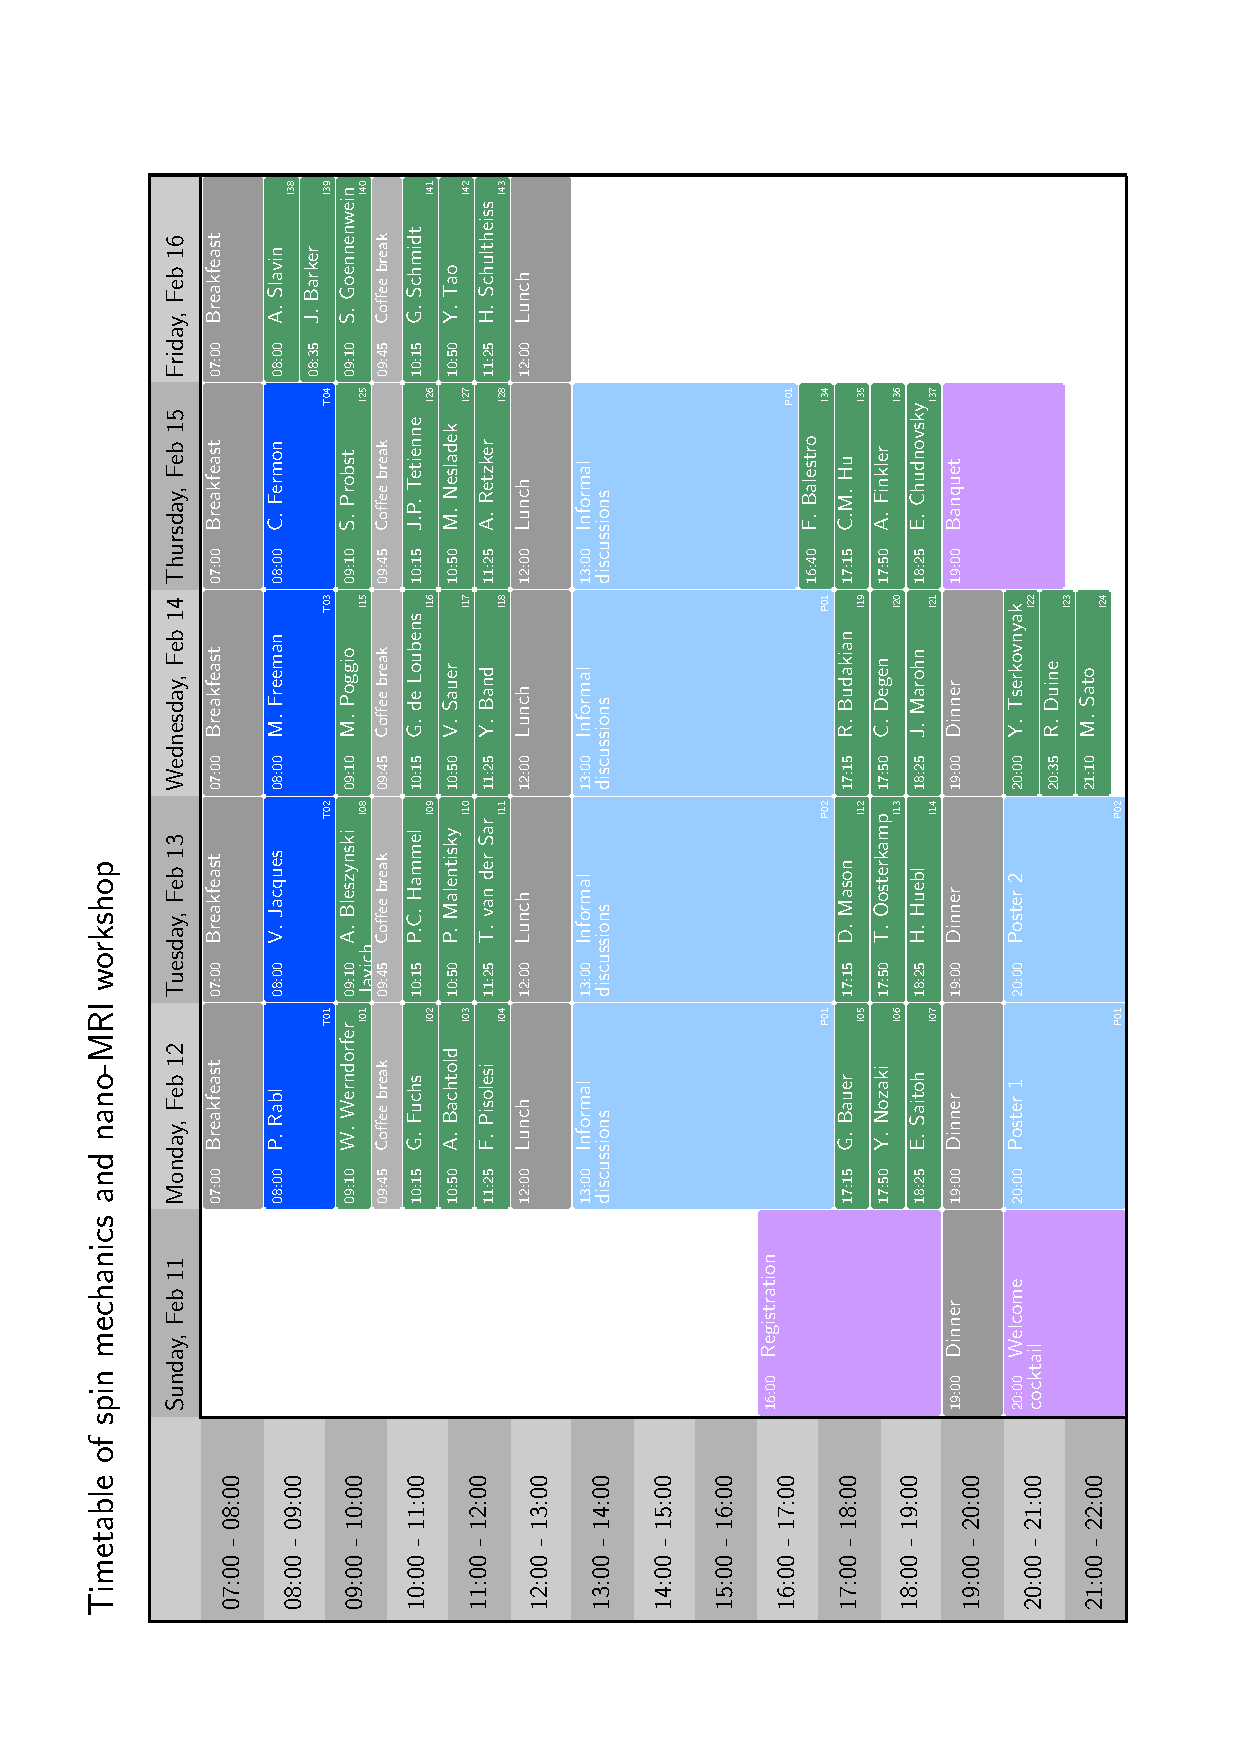
\includepdf[pages={1}]{schedule/schedule.pdf}
\newpage

\begin{tcolorbox}
\textsc{Monday, Feb 12th}
\end{tcolorbox}

\begin{minipage}[t]{.2\textwidth} %
\vskip -8pt \color{red} 8:00 - 9:00
\end{minipage} %
\begin{minipage}[t]{.8\textwidth} %
\textit{Tutorial talk}\\ \vskip -8pt
\textbf{Photon mediated non-local manipulation of spin current using
microwave cavity} \\  \vskip -8pt
James T. Kirk\\
Star Fleet Entreprise\\
\end{minipage}

\begin{minipage}[t]{.2\textwidth} %
\vskip -8pt \color{red} 9:00 - 9:35
\end{minipage} %
\begin{minipage}[t]{.8\textwidth} %
\textit{Invited talk}\\ \vskip -8pt
\textbf{Photon mediated non-local manipulation of spin current using
microwave cavity} \\ \vskip -8pt
Spock\\
Star Fleet Entreprise\\
\end{minipage}


\mainmatter
\chapter{Abstracts}
\newpage
\begin{refsection}
\begin{conf-abstract}[Invited Talk\\ 
Day \\ 
XX:XX am]
{Nanoscale detection and hyperpolarisation of nuclear spins using cross-relaxation in diamond}
{\color{blue} Jean-Philippe Tetienne}
{jtetienne@unimelb.edu.au}
{University of Melbourne, School of Physics, Parkville, VIC 3010, Australia}
{\decofourleft \decofourright}
\indexauthors{Tetienne!Jean-Philippe}

The nitrogen-vacancy (NV) centre in diamond is a leading system for the detection and spectroscopy of spins in nanoscale samples. Most sensing schemes rely on driving of the NV spins with pulsed radiofrequency fields to engineer the NV Hamiltonian and make it sensitive to the target spins. In this talk, I will present an alternative approach to sensing that utilises cross-relaxation between the target spins and the probe NV spin, enabling all-optical spectroscopy of nearby electronic and nuclear spins \cite{Hall_2016,Wood_2016,Wood_2017}. I will then show how cross-relaxation can be used to transfer polarisation to the sample, with an efficiency enhanced by up to an order of magnitude over the established Hartmann-Hahn method, leading to the first observation of hyperpolarisation of external spins using a single NV probe \cite{1708.05906v2}. These results suggest that cross-relaxation could be a useful for nanoscale magnetic resonance imaging.

\begin{conf-abstract}[Invited Talk\\ 
Day \\ 
XX:XX am]
{Nanoscale detection and hyperpolarisation of nuclear spins using cross-relaxation in diamond}
{\color{blue} Jean-Philippe Tetienne}
{jtetienne@unimelb.edu.au}
{University of Melbourne, School of Physics, Parkville, VIC 3010, Australia}
{\decofourleft \decofourright}
\indexauthors{Tetienne!Jean-Philippe}

The nitrogen-vacancy (NV) centre in diamond is a leading system for the detection and spectroscopy of spins in nanoscale samples. Most sensing schemes rely on driving of the NV spins with pulsed radiofrequency fields to engineer the NV Hamiltonian and make it sensitive to the target spins. In this talk, I will present an alternative approach to sensing that utilises cross-relaxation between the target spins and the probe NV spin, enabling all-optical spectroscopy of nearby electronic and nuclear spins \cite{Hall_2016,Wood_2016,Wood_2017}. I will then show how cross-relaxation can be used to transfer polarisation to the sample, with an efficiency enhanced by up to an order of magnitude over the established Hartmann-Hahn method, leading to the first observation of hyperpolarisation of external spins using a single NV probe \cite{1708.05906v2}. These results suggest that cross-relaxation could be a useful for nanoscale magnetic resonance imaging.

\begin{conf-abstract}[\input{stamps/Tetienne}]
{Nanoscale detection and hyperpolarisation of nuclear spins using cross-relaxation in diamond}
{\color{blue} Jean-Philippe Tetienne}
{jtetienne@unimelb.edu.au}
{University of Melbourne, School of Physics, Parkville, VIC 3010, Australia}
{\decofourleft \decofourright}
\indexauthors{Tetienne!Jean-Philippe}

\input{abstracts/body/Tetienne}

\input{figs/Tetienne}

\printbibliography[heading=none]

\end{conf-abstract}


\printbibliography[heading=none]

\end{conf-abstract}


\printbibliography[heading=none]

\end{conf-abstract}

\end{refsection}
\begin{refsection}
\begin{conf-abstract}[Poster\\ 
Day \\ 
XX:XX am]
{Superconducting Levitation of Micron-size Ferromagnetic Particle for Sensitive Magnetometry}
{\color{blue} Tao Wang}
{taowang@berkeley.edu}
{University of California, Berkeley, 6116 Columbia Ave, Richmond, CA 94804, United States}
{{\color{blue}Derek Kimball}\\ \textit{Department of Physics, California State University, East Bay, Hayward, California 94542-3084, USA}\\ 
{\color{blue}Alexander Sushkov}\\ \textit{ Department of Physics, Boston University, Boston, Massachusetts 02215, USA}\\ 
{\color{blue}Dmitry Budker}\\ \textit{Department of Physics, University of California, Berkeley, California 94720-7300, USA}\\ 
\decofourleft \decofourright}
\indexauthors{Wang!Tao}

A precessing ferromagnetic needle magnetometer is proposed in \cite{Jackson_Kimball_2016}, comparing with the alkali vapor cell atomic magnetometer. The needle magnetometer has a better fundamental sensitivity due to much higher density and the atoms precess coherently. Based on the theoretical estimate, the needle magnetometer's sensitivity could surpass the standard quantum limit (SQL). The purpose of levitating the ferromagnetic particle is letting the particle freely precess. The Meissner effect of the superconductors is promising for levitation. The flux pinning inside the type-I superconductor (lead) prevents the micro-particle from stable levitation, when the size of the particle is comparable with size of the flux pinning fringe of lead, the micro-particle could be easily attracted by the flux pinning and fall to the surface. The type-II superconductors are usually in mixed state, however, when the type-II superconductor has a large Hc1, and the external magnetic field is below Hc1, then Meissner effect is dominant. Another requirement for observing the needle particle processing about the magnetic field instead of orienting to the magnetic field is the angular momentum of total spins is much larger than the mechanical orbital angular momentum. In this case, the external magnetic field needs to be shielded/compensated. For a 10 um length needle, the field needs to be smaller than 1 nT. Another advantage of the superconducting levitation is that the bowl-shaped superconductor also acts as superconducting magnetic shield. This research could tell the boundary between the classical physics and the quantum physics.

A precessing ferromagnetic needle magnetometer is proposed in \cite{Jackson_Kimball_2016}, comparing with the alkali vapor cell atomic magnetometer. The needle magnetometer has a better fundamental sensitivity due to much higher density and the atoms precess coherently. Based on the theoretical estimate, the needle magnetometer's sensitivity could surpass the standard quantum limit (SQL). The purpose of levitating the ferromagnetic particle is letting the particle freely precess. The Meissner effect of the superconductors is promising for levitation. The flux pinning inside the type-I superconductor (lead) prevents the micro-particle from stable levitation, when the size of the particle is comparable with size of the flux pinning fringe of lead, the micro-particle could be easily attracted by the flux pinning and fall to the surface. The type-II superconductors are usually in mixed state, however, when the type-II superconductor has a large Hc1, and the external magnetic field is below Hc1, then Meissner effect is dominant. Another requirement for observing the needle particle processing about the magnetic field instead of orienting to the magnetic field is the angular momentum of total spins is much larger than the mechanical orbital angular momentum. In this case, the external magnetic field needs to be shielded/compensated. For a 10 um length needle, the field needs to be smaller than 1 nT. Another advantage of the superconducting levitation is that the bowl-shaped superconductor also acts as superconducting magnetic shield. This research could tell the boundary between the classical physics and the quantum physics.

\printbibliography[heading=none]

\end{conf-abstract}

\end{refsection}
\begin{refsection}
\begin{conf-abstract}[Invited Talk\\ 
Day \\ 
XX:XX am]
{Deeply nonlinear ferromagnetic resonance in a YIG nano-disk:  MRFM spectroscopy of spin-wave instabilities}
{\color{blue} Grégoire de Loubens}
{gregoire.deloubens@cea.fr}
{Service de Physique de l'Etat Condensé, CEA, CNRS, Université Paris-Saclay, Orme des Mersisiers, CEA Saclay, 91191 Gif-sur-Yvette, France}
{{\color{blue}Y. Li, V. Naletov}\\ \textit{SPEC, CEA, CNRS, Université Paris-Saclay, 91191 Gif-sur-Yvette, France}\\ 
{\color{blue}O. Klein}\\ \textit{ SPINTEC, CEA, CNRS and Université Grenoble Alpes, 38054 Grenoble, France}\\ 
{\color{blue}P. Bortolotti, V. Cros, A. Anane}\\ \textit{Unité Mixte de Physique CNRS, Thales, Univ. Paris-Sud, Université Paris-Saclay, 91767 Palaiseau, France}\\ 
\decofourleft \decofourright}
\indexauthors{de Loubens!Grégoire}

Magnetization dynamics is strongly nonlinear, yielding a series of interesting phenomena. It is well known that in ferromagnetic resonance of extended films, spin-wave (SW) instabilities quickly develop as the excitation power is increased \cite{Suhl_1957}, preventing to achieve large angle of uniform precession. The situation is quite different in nanostructures, where SW modes are highly quantized due to the geometric confinement, and expected to influence less the magnetization dynamics in the nonlinear regime. In this work, we probe the magnetization dynamics of an ultra-low damping YIG nano-disk \cite{Hahn_2014} using magnetic resonance force microscopy (MRFM). Ultra-large amplitude precession with complete suppression of the longitudinal component is achieved by pumping the sample with a uniform microwave field. Strikingly, we measure that the foldover shift is not constantly growing as the power is increased, but instead presents plateaus, pointing towards nonlinear energy dissipation to quantized SW modes, which is confirmed by micromagnetic simulations. In addition, by applying a second microwave field we are able to excite the SW resonances in the large-amplitude precession state. The lowest energy mode corresponds to the uniform nutation of the magnetization about its stable precession trajectory, whose frequency was shown to have a similar form as the Rabi formula, generalized to take into account nonlinearities \cite{Bertotti_2001}. Micromagnetic simulations show that higher order modes are nutation modes with spatial gradients, i.e., SW nutation modes.

Magnetization dynamics is strongly nonlinear, yielding a series of interesting phenomena. It is well known that in ferromagnetic resonance of extended films, spin-wave (SW) instabilities quickly develop as the excitation power is increased \cite{Suhl_1957}, preventing to achieve large angle of uniform precession. The situation is quite different in nanostructures, where SW modes are highly quantized due to the geometric confinement, and expected to influence less the magnetization dynamics in the nonlinear regime. In this work, we probe the magnetization dynamics of an ultra-low damping YIG nano-disk \cite{Hahn_2014} using magnetic resonance force microscopy (MRFM). Ultra-large amplitude precession with complete suppression of the longitudinal component is achieved by pumping the sample with a uniform microwave field. Strikingly, we measure that the foldover shift is not constantly growing as the power is increased, but instead presents plateaus, pointing towards nonlinear energy dissipation to quantized SW modes, which is confirmed by micromagnetic simulations. In addition, by applying a second microwave field we are able to excite the SW resonances in the large-amplitude precession state. The lowest energy mode corresponds to the uniform nutation of the magnetization about its stable precession trajectory, whose frequency was shown to have a similar form as the Rabi formula, generalized to take into account nonlinearities \cite{Bertotti_2001}. Micromagnetic simulations show that higher order modes are nutation modes with spatial gradients, i.e., SW nutation modes.

\printbibliography[heading=none]

\end{conf-abstract}

\end{refsection}
\begin{refsection}
\begin{conf-abstract}[Invited Talk\\ 
Day \\ 
XX:XX am]
{High-resolution nanoscale nuclear magnetic resonance imaging and spectroscopy}
{\color{blue} Raffi Budakian}
{rbudakian@uwaterloo.ca}
{University of Waterloo, Department of Physics and Institute for Quantum Computing, 200 University Ave. W, Waterloo, ON N2L3G1, Canada}
{{\color{blue}William Rose, Holger Haas, and David Cory}\\ \textit{200 University Ave. W, Waterloo ON, N2L3G1}\\ 
\decofourleft \decofourright}
\indexauthors{Budakian!Raffi}

I will present a new method for high-resolution nanoscale magnetic resonance imaging that combines the high spin sensitivity of nanowire-based force detection with the high spectral resolution of NMR spectroscopy. I will discuss the development of NMR pulses designed using optimal control theory (OCT) that enable high fidelity unitary operations to be implemented on nanoscale nuclear spin ensembles.  One important capability in the realization high fidelity spin control is the ability to control the average spin Hamiltonians during the unitary evolution.  Using OCT pulses that incorporate average Hamiltonian theory, we demonstrate a factor of 500 reduction of the proton spin resonance linewidth in a (50~nm)$^3$ volume of polystyrene, and image proton spins in one dimension with a spatial resolution below 2~nm \cite{1707.01062v1}. I will discuss the application of these ideas to harness a broad range of high-resolution NMR techniques in the nano-MRI setting.

I will present a new method for high-resolution nanoscale magnetic resonance imaging that combines the high spin sensitivity of nanowire-based force detection with the high spectral resolution of NMR spectroscopy. I will discuss the development of NMR pulses designed using optimal control theory (OCT) that enable high fidelity unitary operations to be implemented on nanoscale nuclear spin ensembles.  One important capability in the realization high fidelity spin control is the ability to control the average spin Hamiltonians during the unitary evolution.  Using OCT pulses that incorporate average Hamiltonian theory, we demonstrate a factor of 500 reduction of the proton spin resonance linewidth in a (50~nm)$^3$ volume of polystyrene, and image proton spins in one dimension with a spatial resolution below 2~nm \cite{1707.01062v1}. I will discuss the application of these ideas to harness a broad range of high-resolution NMR techniques in the nano-MRI setting.

\printbibliography[heading=none]

\end{conf-abstract}

\end{refsection}
\begin{refsection}
\begin{conf-abstract}[Invited Talk\\ 
Day \\ 
XX:XX am]
{Alternating spin current generation in Cu thin film by injecting surface acoustic waves}
{\color{blue} Yukio Nozaki}
{nozaki@phys.keio.ac.jp}
{Keio University, Yokohama 223-8522, Japan}
{{\color{blue}D. Kobayashi and T. Yoshikawa}\\ \textit{Keio University, Yokohama 223-8522, Japan}\\ 
{\color{blue}S. Maekawa}\\ \textit{ Japan Atomic Energy Agency, Tokai 319-1195, Japan}\\ 
{\color{blue}M. Matsuo, R. Iguchi and E. Saitoh}\\ \textit{Tohoku University, Sendai 980-8577, Japan}\\ 
\decofourleft \decofourright}
\indexauthors{Nozaki!Yukio}

Spin angular momentum which is one of the degrees of freedom in electron can be mutually converted with a macroscopic rotation according to the conservation low of angular momentum. The conversion from the spin angular momentum to the macroscopic rotation was experimentally demonstrated in ferromagnetic bodies by Einstein and De Haas while Barnett succeeded its inverse conversion. Very recently, from the analytical solution of the Dirac equation with a general covariance, Matsuo et al. theoretically predicted that the same kind of mutual conversion can be realized for free electrons in non-magnetic metals with a weak spin orbital coupling \cite{Matsuo_2013}. We demonstrated a conversion of alternating spin current (SC) from a macroscopic rotation generated by surface acoustic wave (SAW) which propagates in a NiFe / Cu bilayer deposited on a LiNbO$_3$ substrate \cite{Kobayashi_2017} \. An FMR excited in the NiFe layer was successfully observed when the fundamental frequency of SAW matched with the FMR frequency. The strength of FMR excitation was strongly suppressed when the Cu layer was removed from the bilayer or an insulating SiO$_2$ layer was inserted in the interface of the bilayer. This is the clear evidence that the alternating SC generated in Cu layer via spin-rotation coupling (SRC) plays an important role for the FMR excitation. The angular dependence of the strength of FMR excitation quantitatively supports the successful generation of alternating SC using SAW via SRC. Our experimental result will open the way to generate an alternating SC in variety of SAW devices without using ferromagnets and/or nonmagnetic materials with large spin-orbital coupling.

Invited Talk\\ 
Day \\ 
XX:XX am

\printbibliography[heading=none]

\end{conf-abstract}

\end{refsection}
\begin{refsection}
\begin{conf-abstract}[Invited Talk\\ 
Day \\ 
XX:XX am]
{Dynamics of a Magnetic Needle in a Magnetic field: Magnetometer Sensitivity to Landau--Lifshitz--Gilbert Damping}
{\color{blue} Yehuda Band}
{band@bgu.ac.il}
{Ben-Gurion University, P.O.B. 653 Beer-Sheva 8410501, Israel, Israel}
{{\color{blue}Y. Avishai}\\ \textit{P.O.B. 653 Beer-Sheva 8410501, Israel}\\ 
{\color{blue}A. Shnirman}\\ \textit{ Institut fur Theorie der Kondensierten Materie, Karlsruhe Institute of Technology, D-76128 Karlsruhe, Germany}\\ 
\decofourleft \decofourright}
\indexauthors{Band!Yehuda}

Recently, it was predicted that the sensitivity of a precessing magnetic needle magnetometer can surpass that of present state-of-the-art magnetometers by several orders of magnitude \cite{Jackson_Kimball_2016}.  In order to model the dynamics of a single-domain magnetic needle in a magnetic field, the dissipation of spin components not along the axis of easiest magnetization must be taken into account \cite{Gilbert_2004}. Where there is dissipation, fluctuations are also present \cite{Callen_1951}.  Fluctuations are a source of uncertainty that can affect the accuracy of the magnetometer.  We calculate the dynamics of a magnetic needle in the presence of an external magnetic field and determine the uncertainty of a magnetic needle magnetometer due to the fluctuations that give rise to Gilbert damping \cite{Gilbert_2004}, i.e., interactions with internal degrees of freedom such as lattice vibrations, spin waves, and thermal electric currents.  We solve the Heisenberg equations of motion for the spin, ${\hat {\bf S}}$, the unit vector in the direction of the axis of easiest magnetization, ${\hat {\bf n}}$, and the total angular momentum,  ${\hat {\bf J}}$, in mean-field approximation \cite{Band_2013}  by taking quantum expectation values of the equations, and noting that for large spin and orbital angular momentum, the standard deviation is small compared to the quantum average.   When fluctuations are included, numerical solution of the stochastic equations is difficult when the anisotropy coefficient is large.  Therefore we develop a perturbative solution around the adiabatic solution.  Analysis of the uncertainty in such magnetic field measurements in the limit of small and large magnetic fields will be presented.

\begin{conf-abstract}[Invited Talk\\ 
Day \\ 
XX:XX am]
{Dynamics of a Magnetic Needle in a Magnetic field: Magnetometer Sensitivity to Landau--Lifshitz--Gilbert Damping}
{\color{blue} Yehuda Band}
{band@bgu.ac.il}
{Ben-Gurion University, P.O.B. 653 Beer-Sheva 8410501, Israel, Israel}
{{\color{blue}Y. Avishai}\\ \textit{P.O.B. 653 Beer-Sheva 8410501, Israel}\\ 
{\color{blue}A. Shnirman}\\ \textit{ Institut fur Theorie der Kondensierten Materie, Karlsruhe Institute of Technology, D-76128 Karlsruhe, Germany}\\ 
\decofourleft \decofourright}
\indexauthors{Band!Yehuda}

Recently, it was predicted that the sensitivity of a precessing magnetic needle magnetometer can surpass that of present state-of-the-art magnetometers by several orders of magnitude \cite{Jackson_Kimball_2016}.  In order to model the dynamics of a single-domain magnetic needle in a magnetic field, the dissipation of spin components not along the axis of easiest magnetization must be taken into account \cite{Gilbert_2004}. Where there is dissipation, fluctuations are also present \cite{Callen_1951}.  Fluctuations are a source of uncertainty that can affect the accuracy of the magnetometer.  We calculate the dynamics of a magnetic needle in the presence of an external magnetic field and determine the uncertainty of a magnetic needle magnetometer due to the fluctuations that give rise to Gilbert damping \cite{Gilbert_2004}, i.e., interactions with internal degrees of freedom such as lattice vibrations, spin waves, and thermal electric currents.  We solve the Heisenberg equations of motion for the spin, ${\hat {\bf S}}$, the unit vector in the direction of the axis of easiest magnetization, ${\hat {\bf n}}$, and the total angular momentum,  ${\hat {\bf J}}$, in mean-field approximation \cite{Band_2013}  by taking quantum expectation values of the equations, and noting that for large spin and orbital angular momentum, the standard deviation is small compared to the quantum average.   When fluctuations are included, numerical solution of the stochastic equations is difficult when the anisotropy coefficient is large.  Therefore we develop a perturbative solution around the adiabatic solution.  Analysis of the uncertainty in such magnetic field measurements in the limit of small and large magnetic fields will be presented.

\begin{conf-abstract}[\input{stamps/Band}]
{Dynamics of a Magnetic Needle in a Magnetic field: Magnetometer Sensitivity to Landau--Lifshitz--Gilbert Damping}
{\color{blue} Yehuda Band}
{band@bgu.ac.il}
{Ben-Gurion University, P.O.B. 653 Beer-Sheva 8410501, Israel, Israel}
{{\color{blue}Y. Avishai}\\ \textit{P.O.B. 653 Beer-Sheva 8410501, Israel}\\ 
{\color{blue}A. Shnirman}\\ \textit{ Institut fur Theorie der Kondensierten Materie, Karlsruhe Institute of Technology, D-76128 Karlsruhe, Germany}\\ 
\decofourleft \decofourright}
\indexauthors{Band!Yehuda}

\input{abstracts/body/Band}

\input{figs/Band}

\printbibliography[heading=none]

\end{conf-abstract}


\printbibliography[heading=none]

\end{conf-abstract}


\printbibliography[heading=none]

\end{conf-abstract}

\end{refsection}
\begin{refsection}
\begin{conf-abstract}[Invited Talk\\ 
Day \\ 
XX:XX am]
{Current-induced dynamics in antiferromagnets: generation of THz-frequency signals}
{\color{blue} Andrei N. Slavin}
{slavin@oakland.edu}
{Oakland University, 146 Library Drive, Rochester, MI  48309-4479, United States}
{{\color{blue}O. Sulymenko}\\ \textit{Taras Shevchenko National University of Kyiv, Kyiv 01601, Ukraine}\\ 
\decofourleft \decofourright}
\indexauthors{Slavin!Andrei N.}

We propose  a generator of THz-frequency signals based on a layered structure consisting of a current-driven platinum (Pt) layer and a layer of an antiferromagnet (AFM) with easy-plane anisotropy where the magnetization vectors of the AFM sublattices are canted inside the easy plane
due to  the Dzyaloshinskii-Moriya interaction (DMI) \cite{1707.07491v1}. The DC electric current flowing in the Pt layer creates, due to the spin-Hall effect, a perpendicular spin current which, being injected into the AFM layer, tilts the DMI-canted AFM sublattices out of the easy plane, thus exposing them to the action
of a strong internal exchange magnetic field of the AFM. The sublattice magnetizations along with the small net magnetization vector of a canted AFM start to rotate about the hard  anisotropy axis of the AFM with the THz frequency proportional to the injected spin current and a square root of the AFM exchange field. The rotation of the small net magnetization results in the THz -frequency dipolar radiation that can be directly received by an adjacent (e.g. dielectric) resonator. We demonstrate theoretically that the generated frequencies in the range $f = $0.05- 2.0 THz are possible at the experimentally reachable magnitudes of the driving current density, and evaluate the
power of the signal radiated into different types of resonators, showing that this power increases with the increase of the generation frequency $f$.

\begin{conf-abstract}[Invited Talk\\ 
Day \\ 
XX:XX am]
{Current-induced dynamics in antiferromagnets: generation of THz-frequency signals}
{\color{blue} Andrei N. Slavin}
{slavin@oakland.edu}
{Oakland University, 146 Library Drive, Rochester, MI  48309-4479, United States}
{{\color{blue}O. Sulymenko}\\ \textit{Taras Shevchenko National University of Kyiv, Kyiv 01601, Ukraine}\\ 
\decofourleft \decofourright}
\indexauthors{Slavin!Andrei N.}

We propose  a generator of THz-frequency signals based on a layered structure consisting of a current-driven platinum (Pt) layer and a layer of an antiferromagnet (AFM) with easy-plane anisotropy where the magnetization vectors of the AFM sublattices are canted inside the easy plane
due to  the Dzyaloshinskii-Moriya interaction (DMI) \cite{1707.07491v1}. The DC electric current flowing in the Pt layer creates, due to the spin-Hall effect, a perpendicular spin current which, being injected into the AFM layer, tilts the DMI-canted AFM sublattices out of the easy plane, thus exposing them to the action
of a strong internal exchange magnetic field of the AFM. The sublattice magnetizations along with the small net magnetization vector of a canted AFM start to rotate about the hard  anisotropy axis of the AFM with the THz frequency proportional to the injected spin current and a square root of the AFM exchange field. The rotation of the small net magnetization results in the THz -frequency dipolar radiation that can be directly received by an adjacent (e.g. dielectric) resonator. We demonstrate theoretically that the generated frequencies in the range $f = $0.05- 2.0 THz are possible at the experimentally reachable magnitudes of the driving current density, and evaluate the
power of the signal radiated into different types of resonators, showing that this power increases with the increase of the generation frequency $f$.

\begin{conf-abstract}[\input{stamps/Slavin}]
{Current-induced dynamics in antiferromagnets: generation of THz-frequency signals}
{\color{blue} Andrei N. Slavin}
{slavin@oakland.edu}
{Oakland University, 146 Library Drive, Rochester, MI  48309-4479, United States}
{{\color{blue}O. Sulymenko}\\ \textit{Taras Shevchenko National University of Kyiv, Kyiv 01601, Ukraine}\\ 
\decofourleft \decofourright}
\indexauthors{Slavin!Andrei N.}

\input{abstracts/body/Slavin}

\input{figs/Slavin}

\printbibliography[heading=none]

\end{conf-abstract}


\printbibliography[heading=none]

\end{conf-abstract}


\printbibliography[heading=none]

\end{conf-abstract}

\end{refsection}
\begin{refsection}
\begin{conf-abstract}[Invited Talk\\ 
Day \\ 
XX:XX am]
{Tunable spin-polaron state in a singly clamped semiconducting carbon nanotube}
{\color{blue} Fabio Pistolesi}
{fabio.pistolesi@u-bordeaux.fr}
{Université de Bordeaux and CNRS, LOMA, Cours de la liberation, Talence, France}
{{\color{blue}R. Shekhter}\\ \textit{Department of Physics, University of Gothenburg, SE-412 96 Goteborg, Sweden}\\ 
\decofourleft \decofourright}
\indexauthors{Pistolesi!Fabio}

In this talk we consider a semiconducting carbon nanotube (CNT) lying on a ferromagnetic insulating substrate with one end passing the substrate and suspended over a metallic gate. We assume that the polarized substrate induces an exchange interaction acting as a local magnetic field for the electrons in the nonsuspended CNT side.  We show that one can generate electrostatically a tunable spin-polarized polaronic state localized at the bending end of the CNT. We argue that at low temperatures manipulation and detection of the localized quantum spin state are possible (see also \cite{Pistolesi_2015}).

In this talk we consider a semiconducting carbon nanotube (CNT) lying on a ferromagnetic insulating substrate with one end passing the substrate and suspended over a metallic gate. We assume that the polarized substrate induces an exchange interaction acting as a local magnetic field for the electrons in the nonsuspended CNT side.  We show that one can generate electrostatically a tunable spin-polarized polaronic state localized at the bending end of the CNT. We argue that at low temperatures manipulation and detection of the localized quantum spin state are possible (see also \cite{Pistolesi_2015}).

\printbibliography[heading=none]

\end{conf-abstract}

\end{refsection}
\begin{refsection}
\begin{conf-abstract}[Invited Talk\\ 
Day \\ 
XX:XX am]
{Ultrafast Spintronics with Topological Lasers}
{\color{blue} Masahiro Sato}
{masahiro.sato.phys@vc.ibaraki.ac.jp}
{Ibaraki University, 2-1-1 Bunkyo, Mito, Ibaraki 310-8512, Japan, Japan}
{{\color{blue}H. Fujita}\\ \textit{Institute for Solid State Physics, University of Tokyo, Kashiwa 277-8581, Japan}\\ 
\decofourleft \decofourright}
\indexauthors{Sato!Masahiro}

Optical vortex (or vortex beam) is the singular laser beam carrying an intrinsic orbital angular momentum, \cite{Allen_1992} and has been actively studied especially as a new tool to control various kinds of matter. Due to the presence of the angular momentum, the vortex beam has a characteristic spatial distribution of electromagnetic fields. Making use of the spatial features, we theoretically propose new ways of generating/controlling magnetic nanostructures such as skyrmions and skyrmioniums \cite{Fert_2013} in magnets with vortex beams. We concentrate on two set ups: Applications of high- (ultraviolet, visible) and low-frequency (Tera Hz: THz) vortex beams to magnets. In the case of the high-frequency beam, its oscillation is too faster for typical spin dynamics and the spins cannot be directly coupled to the oscillating fields, while spins can feel heating driven by the beam. Based on Landau-Lifshitz-Gilbert (LLG) equation with the beam-driven heating, we show that vortex beams in ultraviolet or visible range can generate multiple ring-shape magnetic defects such as skyrmionium in chiral magnets. \cite{Fujita_2017} On the other hand, when we apply THz vortex beams to magnets, the direct coupling between the spins and the electromagnetic fields becomes relevant and richer spin dynamics occur. We show from the LLG simulation that the magnetic resonance driven by THz vortex beam in usual ferromagnets leads to a nanostructure with a finite spin scalar chirality, \cite{Fujita_2017a} and it indicates the possibility of vortex-beam driven Hall effect in metallic magnets. We also show that THz vortex beam can simultaneously generate multiple skyrmions in chiral ferromagnets, depending on the value of the angular momentum, \cite{Fujita_2017a} if the beams are sufficiently focusing beyond its diffraction limit with near-field techniques. In the talk, I would like to carefully report the essential aspects of our proposal.

Optical vortex (or vortex beam) is the singular laser beam carrying an intrinsic orbital angular momentum, \cite{Allen_1992} and has been actively studied especially as a new tool to control various kinds of matter. Due to the presence of the angular momentum, the vortex beam has a characteristic spatial distribution of electromagnetic fields. Making use of the spatial features, we theoretically propose new ways of generating/controlling magnetic nanostructures such as skyrmions and skyrmioniums \cite{Fert_2013} in magnets with vortex beams. We concentrate on two set ups: Applications of high- (ultraviolet, visible) and low-frequency (Tera Hz: THz) vortex beams to magnets. In the case of the high-frequency beam, its oscillation is too faster for typical spin dynamics and the spins cannot be directly coupled to the oscillating fields, while spins can feel heating driven by the beam. Based on Landau-Lifshitz-Gilbert (LLG) equation with the beam-driven heating, we show that vortex beams in ultraviolet or visible range can generate multiple ring-shape magnetic defects such as skyrmionium in chiral magnets. \cite{Fujita_2017} On the other hand, when we apply THz vortex beams to magnets, the direct coupling between the spins and the electromagnetic fields becomes relevant and richer spin dynamics occur. We show from the LLG simulation that the magnetic resonance driven by THz vortex beam in usual ferromagnets leads to a nanostructure with a finite spin scalar chirality, \cite{Fujita_2017a} and it indicates the possibility of vortex-beam driven Hall effect in metallic magnets. We also show that THz vortex beam can simultaneously generate multiple skyrmions in chiral ferromagnets, depending on the value of the angular momentum, \cite{Fujita_2017a} if the beams are sufficiently focusing beyond its diffraction limit with near-field techniques. In the talk, I would like to carefully report the essential aspects of our proposal.

\printbibliography[heading=none]

\end{conf-abstract}

\end{refsection}
\begin{refsection}
\begin{conf-abstract}[Invited Talk\\ 
Day \\ 
XX:XX am]
{Quantum Control Over Diamond Nitrogen-Vacancy Centers Using a Mechanical Resonator}
{\color{blue} Gregory Fuchs}
{gdf9@cornell.edu}
{Cornell University, 228 Clark Hall, Cornell University, Ithaca, NY 14853, United States}
{{\color{blue}E. R. MacQuarrie, H. Chen, M. Otten and T. Gosavi}\\ \textit{Cornell University, Ithaca, NY 14853, United States}\\ 
{\color{blue}S. Bhave}\\ \textit{ Purdue University, West Laffayette, IN 47907, United States}\\ 
\decofourleft \decofourright}
\indexauthors{Fuchs!Gregory}

Creating and studying coherent interactions between solid-state qubits and mechanical resonators is a challenge at the intersection of atomic physics, condensed matter physics, and engineering. Furthermore, there is growing consensus that mechanical motion is a “plastic” degree of freedom for solid-state qubits, with the potential to form a interface between spins, photons and phonons.  This has motivated intense research into the coherent interactions between mechanical resonators and qubits formed from photons, trapped atoms, superconducting circuits, quantum dots, and nitrogen-vacancy (NV) centers in diamond, to name a few.  I will describe our experiments to coherently control NV center spins through their coupling to the dynamic crystal lattice strain of a gigahertz-frequency mechanical resonator.  In high-quality diamond mechanical resonators, we demonstrate coherent Rabi oscillations of NV center spins driven by mechanical motion instead of an oscillating magnetic field \cite{MacQuarrie_2013,MacQuarrie_2015}. Furthermore, we show that a mechanical resonator is a resource to prolog the NV center’s spin coherence \cite{MacQuarrie_2015}.  Finally, we examine how resonator strain can couple to NV centers through their excited-state, using either spin-strain coupling at room temperature \cite{MacQuarrie_2017} or orbital-strain coupling low temperature.

Invited Talk\\ 
Day \\ 
XX:XX am

\printbibliography[heading=none]

\end{conf-abstract}

\end{refsection}
\begin{refsection}
\begin{conf-abstract}[Invited Talk\\ 
Day \\ 
XX:XX am]
{Magnetic Resonance of Correlated Spins using a Single Spin Sensor}
{\color{blue} Amit Finkler}
{amit.finkler@weizmann.ac.il}
{Weizmann Institute of Science, 234 Herzl St., Rehovot 7610001, Israel}
{{\color{blue}L. Schlipf, D. Dasari, B. Kern, K. Xu, M. Ternes and K. Kern}\\ \textit{Max Planck Institute for Solid State Physics, Heisenbergstr. 1, 70569 Stuttgart, Germany}\\ 
{\color{blue}T. Oeckinghaus, A. Zappe, J. Wrachtrup}\\ \textit{ 3. Physikalisches Institut, Universität Stuttgart, Pfaffenwaldring 57, 70569 Stuttgart, Germany}\\ 
{\color{blue}Mzkhailo Azarkh and Malte Drescher}\\ \textit{University of Konstanz, Universitätsstr. 10, 78457 Konstanz, Germany}\\ 
\decofourleft \decofourright}
\indexauthors{Finkler!Amit}

With recent reports on the sensing of electron spins and nuclear spins
from single proteins using the nitrogen-vacancy center in diamond, we
attempt to constrain the number of participating spins. This is achieved
by using doubly spin-labeled amino acids. Both room temperature and low
temperature measurements are presented. We also show how one can gauge
the dipolar couplng between a pair of spin labels in the limit of a very
small ($<4$) amount of molecules \cite{Schlipf_2017}. This is an almost mandatory
requirement for sensing spins in more complex (and of interest for
active research) molecules. Finally, we stress the importance of
quantum-assisted methods in reducing the effective measurement time,
which is critical for imaging purposes \cite{H_berle_2017}.

Invited Talk\\ 
Day \\ 
XX:XX am

\printbibliography[heading=none]

\end{conf-abstract}

\end{refsection}
\begin{refsection}
\begin{conf-abstract}[Invited Talk\\ 
Day \\ 
XX:XX am]
{Electrically Detected Magnetic Resonance of NV Spin States in Diamond: Towards Coherent Driving and readout of Single Spin Qubits}
{\color{blue} Milos Nesladek}
{milos.nesladek@uhasselt.be}
{University Hasselt and IMEC, Milos Nesladek ( invited), Belgium}
{\decofourleft \decofourright}
\indexauthors{Nesladek!Milos}

Scalable principles for quantum state readout are one of open questions in quantum technology. Building on the recent results of photoelectric detection of magnetic resonances (PDMR) \cite{Bourgeois_2015,Gulka_2017} we discuss the prospect of PDMR technique for solid-state qubit devices in diamond. One of the key PDMR advantages over the optical detected magnetic resonance  (ODMR) technique are the high detection rates $\sim 5 \times 10^9$ sec$^{-1}$, exceeding orders of magnitude ODMR. Consequently, the novel detection technique might lead to the single shot readout of the NV centres quantum state and provide fast data acquisition at room temperature.  To achieve this goal we discuss the photoelectric gain, used to obtain high detection rates on small NV spin qubit ensembles. The photophysics of the transitions on NV centre is reviewed and several scenarios for obtaining highest single/noise ratio are presented. We demonstrate pulsed PDMR measurements, compatible with coherent manipulation of the spin states realized on quantum chips. Finally we realize a single NV qubits read electrically.
We discuss another defects such as NiV as a potential candidate for electrically read spin qubits in diamond.

Invited Talk\\ 
Day \\ 
XX:XX am

\printbibliography[heading=none]

\end{conf-abstract}

\end{refsection}
\begin{refsection}
\begin{conf-abstract}[Invited Talk\\ 
Day \\ 
XX:XX am]
{Cavity Spintronics}
{\color{blue} Can-Ming Hu}
{hu@physics.umanitoba.ca}
{University of Manitoba, University of Manitoba, Winnipeg, R3T 2N2, Canada}
{\decofourleft \decofourright}
\indexauthors{Hu!Can-Ming}

Cavity Spintronics (also known as Spin Cavitronics) is a newly developing interdisciplinary field that brings together microwave cavity community with researchers from spintronics. This field started around 2014 when it was found that ferromagnets in cavities hybridize with both microwaves and light via light-matter interaction. Since then, the emergence of this field has attracted broad interests. At the center stage of the topic is the physics of a quasi-particle called cavity magnon polariton (CMP). Via the quantum physics of spin-photon entanglement on the one hand, and via classical electrodynamic coupling on the other, CMP connects some of the most exciting modern physics, such as quantum information and quantum optics, with one of the oldest science on the earth, the magnetism. 

In this new community, most groups utilize the hybrid and nonlocal nature of CMP to develop cavity-mediated coupling techniques for both spintronic and quantum applications. This stream of research, including our recent demonstration of cavity-mediated distant control of spin current \cite{Bai_2017}, root on single-particle physics of CMP. In this talk, we will present a distinct feedback-coupled cavity technique, which we develop to study the cooperative dynamics of trillions of CMP. Utilizing such coherent dynamics of CMP ensembles, we demonstrate the control of magnon-photon Rabi frequency by changing the photon Fock state occupation, and we discover the evolution of CMP to cavity magnon triplet and cavity magnon quintuplet [Nature Comm. (2017), to be published]. Our results may open up new avenues for exploiting the light-matter interactions.

Invited Talk\\ 
Day \\ 
XX:XX am

\printbibliography[heading=none]

\end{conf-abstract}

\end{refsection}
\begin{refsection}
\begin{conf-abstract}[Poster\\ 
Day \\ 
XX:XX am]
{Level attraction in a microwave optomechanical circuit}
{\color{blue} Nathan Bernier}
{nathan.bernier@epfl.ch}
{Ecole Polytechnique Fédérale de Lausanne (EPFL), EPFL SB IPHYS LPQM1, PH D3 315, Station 3, 1015 Lausanne, Switzerland}
{{\color{blue}L. D. Tóth, A. K. Feofanov and T. J. Kippenberg}\\ \textit{Ecole Polytechnique Fédérale de Lausanne (EPFL), CH-1015 Lausanne, Switzerland}\\ 
\decofourleft \decofourright}
\indexauthors{Bernier!Nathan}

Level repulsion (the opening of a gap between two degenerate modes due to coupling)
  is ubiquitous anywhere
  from solid state theory to quantum chemistry. 
  In contrast, 
  the mode frequencies can attract instead
  if, for instance,
  one of the modes has negative energy.
  The frequencies converge and develop imaginary components,
  leading to an instability;
  an exceptional point marks the transition.
  This, however, only occurs if
  the dissipation rates of the two modes are equal.
  We expose a theoretical framework for the process and
  realize it experimentally
  through engineered dissipation
  in a multimode superconducting microwave optomechanical circuit~%
  \cite{1709.02220v1}.
  Level attraction is observed 
  for a mechanical oscillator and a superconducting microwave cavity.
  An auxiliary cavity is used to tune the effective
  mechanical dissipation rate to match that of the the microwave cavity
  using sideband cooling.
  Two exceptional points are demonstrated that
  could be exploited for their topological properties.

Level repulsion (the opening of a gap between two degenerate modes due to coupling)
  is ubiquitous anywhere
  from solid state theory to quantum chemistry. 
  In contrast, 
  the mode frequencies can attract instead
  if, for instance,
  one of the modes has negative energy.
  The frequencies converge and develop imaginary components,
  leading to an instability;
  an exceptional point marks the transition.
  This, however, only occurs if
  the dissipation rates of the two modes are equal.
  We expose a theoretical framework for the process and
  realize it experimentally
  through engineered dissipation
  in a multimode superconducting microwave optomechanical circuit~%
  \cite{1709.02220v1}.
  Level attraction is observed 
  for a mechanical oscillator and a superconducting microwave cavity.
  An auxiliary cavity is used to tune the effective
  mechanical dissipation rate to match that of the the microwave cavity
  using sideband cooling.
  Two exceptional points are demonstrated that
  could be exploited for their topological properties.

\printbibliography[heading=none]

\end{conf-abstract}

\end{refsection}
\begin{refsection}
\begin{conf-abstract}[Attendee\\ 
Day \\ 
XX:XX am]
{Quantum Einstein-de Haas Effect studied with molecular spintronic devices}
{\color{blue} Hannes Seeger}
{hannes.seeger@kit.edu}
{Karlsruhe Institute of Technology (KIT), Institute of Physics, Wolfgang-Gaede-Str. 1, D-76131 Karlsruhe, Germany}
{{\color{blue}M. Ganzhorn, J. Schoenle and W. Wernsdorfer}\\ \textit{Institut Néel, CNRS, BP 166, 38042 Grenoble, France}\\ 
{\color{blue}S. Klyatskaya and M.Ruben and W. Wernsdorfer}\\ \textit{ Institut of Nanotechnology (INT), Karlsruhe Institute of Technology (KIT), 76344 Eggenstein-Leopoldshafen, Germany}\\ 
{\color{blue}W. Wernsdorfer}\\ \textit{Institut of Physics, Karlsruhe Institute of Technology (KIT), 76131 Karlsruhe, Germany}\\ 
\decofourleft \decofourright}
\indexauthors{Seeger!Hannes}

One hundred years ago it has been discovered that a change of magnetization in a macroscopic magnetic object results in a mechanical rotation of this magnet. The effect, known as Einstein-de Haas or Richardson effect, demonstrates that a spin angular momentum in the magnet compensates for the mechanical angular momentum associated with its rotation.\cite{Richardson_1908} The experiment is therefore a macroscopic manifestation of the conservation of total angular momentum and energy of electronic spins. According to Noether's theorem, conservation of angular momentum follows from a system's rotational invariance and would be valid for the ensemble of spins in a macroscopic ferromagnet as well as for an individual spin. It has been recently proposed that single spin systems would therefore manifest an Einstein-de Haas effect at the quantum level.\cite{Chudnovsky_1994,Garanin_2011} 

We propose the first experimental realization of a quantum Einstein-de Haas experiment and describe a macroscopic manifestation of the conservation of total angular momentum in individual spins, using a TbPc$_2$ single molecule magnet coupled to a nanomechanical resonator.\cite{Ganzhorn_2013} We demonstrate that the spin associated with the single molecule magnet is then subject to conservation of total angular momentum and energy which results in a total suppression of the molecule's quantum tunneling of magnetization.\cite{Ganzhorn_2016}

Attendee\\ 
Day \\ 
XX:XX am

\printbibliography[heading=none]

\end{conf-abstract}

\end{refsection}
\begin{refsection}
\begin{conf-abstract}[Invited Talk\\ 
Day \\ 
XX:XX am]
{Atomistic spin dynamics of magnetic insulators}
{\color{blue} Joseph Barker}
{joseph.barker@imr.tohoku.ac.jp}
{Institute for Materials Research, Tohoku University, Sendai 980-8577, Japan}
{{\color{blue}G.E.W. Bauer}\\ \textit{Institute for Materials Research, Tohoku University, Sendai 980-0011}\\ 
{\color{blue}S. Maehrlein and T. Kampfrath}\\ \textit{ Fritz Haber Institute of the Max Planck Society, Faradayweg 4-6, 14195 Berlin, Germany}\\ 
\decofourleft \decofourright}
\indexauthors{Barker!Joseph}

Atomistic spin dynamics is a classical formalism in which dynamics and thermodynamics of magnetic materials can be calculated. We focus our studies on magnetic insulators such as yttrium iron garnet (YIG) which is ubiquitous in the insulator spintronics, magnonics and spin mechanics communities. We have extended the classical spin dynamics formalism into the `semi-classical` limit such that the magnons obey quantum statistics whilst the spins remain classical objects. This leads to a vast improvement in the quantitative calculation of material properties such as the magnon heat capacity. We will show recent progress in the calculation of magnon transport properties. We also present experimental evidence and a simple model for a spin-phonon interaction in the THz regime where the phonon excitation dynamically modifies the super exchange coupling leading to a transfer of spin angular moment between the two sublattices \cite{1710.02700v1}. This causes the sublattice magnetization to decrease but maintains the total magnetization through angular momentum conservation.

\begin{conf-abstract}[Invited Talk\\ 
Day \\ 
XX:XX am]
{Atomistic spin dynamics of magnetic insulators}
{\color{blue} Joseph Barker}
{joseph.barker@imr.tohoku.ac.jp}
{Institute for Materials Research, Tohoku University, Sendai 980-8577, Japan}
{{\color{blue}G.E.W. Bauer}\\ \textit{Institute for Materials Research, Tohoku University, Sendai 980-0011}\\ 
{\color{blue}S. Maehrlein and T. Kampfrath}\\ \textit{ Fritz Haber Institute of the Max Planck Society, Faradayweg 4-6, 14195 Berlin, Germany}\\ 
\decofourleft \decofourright}
\indexauthors{Barker!Joseph}

Atomistic spin dynamics is a classical formalism in which dynamics and thermodynamics of magnetic materials can be calculated. We focus our studies on magnetic insulators such as yttrium iron garnet (YIG) which is ubiquitous in the insulator spintronics, magnonics and spin mechanics communities. We have extended the classical spin dynamics formalism into the `semi-classical` limit such that the magnons obey quantum statistics whilst the spins remain classical objects. This leads to a vast improvement in the quantitative calculation of material properties such as the magnon heat capacity. We will show recent progress in the calculation of magnon transport properties. We also present experimental evidence and a simple model for a spin-phonon interaction in the THz regime where the phonon excitation dynamically modifies the super exchange coupling leading to a transfer of spin angular moment between the two sublattices \cite{1710.02700v1}. This causes the sublattice magnetization to decrease but maintains the total magnetization through angular momentum conservation.

\begin{conf-abstract}[\input{stamps/Barker}]
{Atomistic spin dynamics of magnetic insulators}
{\color{blue} Joseph Barker}
{joseph.barker@imr.tohoku.ac.jp}
{Institute for Materials Research, Tohoku University, Sendai 980-8577, Japan}
{{\color{blue}G.E.W. Bauer}\\ \textit{Institute for Materials Research, Tohoku University, Sendai 980-0011}\\ 
{\color{blue}S. Maehrlein and T. Kampfrath}\\ \textit{ Fritz Haber Institute of the Max Planck Society, Faradayweg 4-6, 14195 Berlin, Germany}\\ 
\decofourleft \decofourright}
\indexauthors{Barker!Joseph}

\input{abstracts/body/Barker}

\input{figs/Barker}

\printbibliography[heading=none]

\end{conf-abstract}


\printbibliography[heading=none]

\end{conf-abstract}


\printbibliography[heading=none]

\end{conf-abstract}

\end{refsection}
\begin{refsection}
\begin{conf-abstract}[Invited Talk\\ 
Day \\ 
XX:XX am]
{Limits on spectral resolution measurements by quantum probes for nano NMR}
{\color{blue} Alex Retzker}
{retzker@phys.huji.ac.il}
{The Hebrew University, Racah Institute of Physics, Edmond J. Safra campus. Danciger B Building, room 203, Hebrew University of Jerusalem, Israel 91904, Israel}
{{\color{blue}Amit Rotem, Tuvia Gefen and Alex Retzker}\\ \textit{The Hebrew University, Racah Institute of Physics Edmond J. Safra campus, Israel}\\ 
{\color{blue}Simon Schmitt and Liam McGuiness and Fedor Jelezko}\\ \textit{ 2Institute for Quantum Optics, Ulm University, Albert-Einstein-Allee 11, Ulm 89081, Germany}\\ 
\decofourleft \decofourright}
\indexauthors{Retzker!Alex}

The limits of frequency resolution in nano NMR experiments have been discussed extensively in recent years. It is believed that there is a crucial difference between the ability to resolve a few frequencies and the precision
of estimating a single one. Whereas the efficiency of single frequency estimation gradually increases with the square root of the number of measurements, the ability to resolve two frequencies is limited by the specific time scale of the probe and cannot be compensated for by extra measurements. In this talk I will show  that the relationship between these quantities is more subtle and both are only limited by the Cramer-Rao bound of a single frequency estimation. The talk is based on \cite{Schmitt_2017,1707.01902v1}.

The limits of frequency resolution in nano NMR experiments have been discussed extensively in recent years. It is believed that there is a crucial difference between the ability to resolve a few frequencies and the precision
of estimating a single one. Whereas the efficiency of single frequency estimation gradually increases with the square root of the number of measurements, the ability to resolve two frequencies is limited by the specific time scale of the probe and cannot be compensated for by extra measurements. In this talk I will show  that the relationship between these quantities is more subtle and both are only limited by the Cramer-Rao bound of a single frequency estimation. The talk is based on \cite{Schmitt_2017,1707.01902v1}.

\printbibliography[heading=none]

\end{conf-abstract}

\end{refsection}
\begin{refsection}
\begin{conf-abstract}[Invited Talk\\ 
Day \\ 
XX:XX am]
{Brillouin Scattering in Cavity Optomagnonics}
{\color{blue} Yaroslav Blanter}
{y.m.blanter@tudelft.nl}
{Kavli Institute of Nanoscience, Delft University of Technology, Lorentzweg 1, 2628CJ Delft, the Netherlands}
{{\color{blue}S. Sharma}\\ \textit{Kavli Institute of Nanoscience, Delft University of Technology, Lorentzweg 1, 2628CJ Delft, the Netherlands}\\ 
{\color{blue}G. E. W. Bauer}\\ \textit{ Institute for Materials Research and WPI-AIMR, Tohoku University, Sendai 980-8577, Japan}\\ 
\decofourleft \decofourright}
\indexauthors{Blanter!Yaroslav}

Brillouin light scattering is an established technique to study magnons, the elementary excitations of a magnet. Its efficiency can be enhanced by cavities that concentrate the light intensity. Here, we theoretically study inelastic scattering of photons by a magnetic sphere that supports optical whispering gallery modes in a plane normal to the magnetization. Magnons with low angular momenta scatter the light in the forward direction with a pronounced asymmetry in the Stokes and the anti-Stokes scattering strength, consistent with earlier studies. Magnons with large angular momenta constitute Damon Eschbach modes are shown to inelastically reflect light. The reflection spectrum contains either a Stokes or anti-Stokes peak, depending on the direction of the magnetization, a selection rule that can be explained by the chirality of the Damon Eshbach magnons. The controllable energy transfer can be used to manage the thermodynamics of the magnet by light \cite{Sharma_2017}. We will also discuss recent developments in magnon cooling and manipulation.

\begin{conf-abstract}[Invited Talk\\ 
Day \\ 
XX:XX am]
{Brillouin Scattering in Cavity Optomagnonics}
{\color{blue} Yaroslav Blanter}
{y.m.blanter@tudelft.nl}
{Kavli Institute of Nanoscience, Delft University of Technology, Lorentzweg 1, 2628CJ Delft, the Netherlands}
{{\color{blue}S. Sharma}\\ \textit{Kavli Institute of Nanoscience, Delft University of Technology, Lorentzweg 1, 2628CJ Delft, the Netherlands}\\ 
{\color{blue}G. E. W. Bauer}\\ \textit{ Institute for Materials Research and WPI-AIMR, Tohoku University, Sendai 980-8577, Japan}\\ 
\decofourleft \decofourright}
\indexauthors{Blanter!Yaroslav}

Brillouin light scattering is an established technique to study magnons, the elementary excitations of a magnet. Its efficiency can be enhanced by cavities that concentrate the light intensity. Here, we theoretically study inelastic scattering of photons by a magnetic sphere that supports optical whispering gallery modes in a plane normal to the magnetization. Magnons with low angular momenta scatter the light in the forward direction with a pronounced asymmetry in the Stokes and the anti-Stokes scattering strength, consistent with earlier studies. Magnons with large angular momenta constitute Damon Eschbach modes are shown to inelastically reflect light. The reflection spectrum contains either a Stokes or anti-Stokes peak, depending on the direction of the magnetization, a selection rule that can be explained by the chirality of the Damon Eshbach magnons. The controllable energy transfer can be used to manage the thermodynamics of the magnet by light \cite{Sharma_2017}. We will also discuss recent developments in magnon cooling and manipulation.

\begin{conf-abstract}[\input{stamps/Blanter}]
{Brillouin Scattering in Cavity Optomagnonics}
{\color{blue} Yaroslav Blanter}
{y.m.blanter@tudelft.nl}
{Kavli Institute of Nanoscience, Delft University of Technology, Lorentzweg 1, 2628CJ Delft, the Netherlands}
{{\color{blue}S. Sharma}\\ \textit{Kavli Institute of Nanoscience, Delft University of Technology, Lorentzweg 1, 2628CJ Delft, the Netherlands}\\ 
{\color{blue}G. E. W. Bauer}\\ \textit{ Institute for Materials Research and WPI-AIMR, Tohoku University, Sendai 980-8577, Japan}\\ 
\decofourleft \decofourright}
\indexauthors{Blanter!Yaroslav}

\input{abstracts/body/Blanter}

\input{figs/Blanter}

\printbibliography[heading=none]

\end{conf-abstract}


\printbibliography[heading=none]

\end{conf-abstract}


\printbibliography[heading=none]

\end{conf-abstract}

\end{refsection}
\begin{refsection}
\begin{conf-abstract}[Invited Talk\\ 
Day \\ 
XX:XX am]
{Ultracoherent Mechanical Oscillators for Quantum Optomechanics and Hybrid Systems}
{\color{blue} David Mason}
{drmason@nbi.ku.dk}
{Niels Bohr Institute, Blegdamsvej 17, 2100 København Ø, Denmark}
{{\color{blue}M. Rossi, J. Chen, Y. Seis, S. Saarinen, Y. Tsaturyan and A. Schliesser}\\ \textit{Niels Bohr Institute, University of Copenhagen, Blegdamsvej 17, Denmark}\\ 
\decofourleft \decofourright}
\indexauthors{Mason!David}

Modern optomechanics has been enabled by the availability of high quality mechanical resonators.  Here, we present ongoing work with recently-pioneered \cite{Tsaturyan_2017} 'ultracoherent' membranes, which exploit phononic engineering and soft-clamping techniques to achieve unprecedented mechanical coherence.  With Q-factors of $10^8$ at room temperature and nearly $10^9$ at T$\sim$10K, these devices enable novel experiments in various regimes.

First, by moderate cryogenic cooling, we can readily achieve quantum cooperativities $C_Q = 4g^2/\kappa\gamma \gg 1$, enabling quantum protocols with a mechanical system whose thermal decoherence rate ($\gamma$) approaches that of trapped ions ($\sim$1 ms).  This should allow, for instance, stroboscopic QND localization of a single mechanical mode, or using a novel multimode device, two-mode mechanical squeezing and entanglement.  Remarkably, these membranes can even achieve $C_Q>1$ without cryogenic cooling, and by integration with low-noise fiber mirrors, achieve a macroscopic room-temperature system capable of quantum behavior.

We also exploit the high Q of these resonators to advance the capabilities of various hybrid systems.  These include electro-optomechanical systems\cite{Bagci_2014} as well as systems in which the membrane motion couples to the collective spin of a room-temperature atomic ensemble\cite{M_ller_2017}.  Finally, our soft-clamping techniques can also be exploited to advance force sensing applications.  Towards this end, we have developed low-mass soft-clamped resonators, which seek to advance scanning force microscopy (in particular, MRFM) by moving beyond the usual tip-as-sensor paradigm, and exploiting our ultracoherent mechanical devices.

Modern optomechanics has been enabled by the availability of high quality mechanical resonators.  Here, we present ongoing work with recently-pioneered \cite{Tsaturyan_2017} 'ultracoherent' membranes, which exploit phononic engineering and soft-clamping techniques to achieve unprecedented mechanical coherence.  With Q-factors of $10^8$ at room temperature and nearly $10^9$ at T$\sim$10K, these devices enable novel experiments in various regimes.

First, by moderate cryogenic cooling, we can readily achieve quantum cooperativities $C_Q = 4g^2/\kappa\gamma \gg 1$, enabling quantum protocols with a mechanical system whose thermal decoherence rate ($\gamma$) approaches that of trapped ions ($\sim$1 ms).  This should allow, for instance, stroboscopic QND localization of a single mechanical mode, or using a novel multimode device, two-mode mechanical squeezing and entanglement.  Remarkably, these membranes can even achieve $C_Q>1$ without cryogenic cooling, and by integration with low-noise fiber mirrors, achieve a macroscopic room-temperature system capable of quantum behavior.

We also exploit the high Q of these resonators to advance the capabilities of various hybrid systems.  These include electro-optomechanical systems\cite{Bagci_2014} as well as systems in which the membrane motion couples to the collective spin of a room-temperature atomic ensemble\cite{M_ller_2017}.  Finally, our soft-clamping techniques can also be exploited to advance force sensing applications.  Towards this end, we have developed low-mass soft-clamped resonators, which seek to advance scanning force microscopy (in particular, MRFM) by moving beyond the usual tip-as-sensor paradigm, and exploiting our ultracoherent mechanical devices.

\printbibliography[heading=none]

\end{conf-abstract}

\end{refsection}
\begin{refsection}
\begin{conf-abstract}[Invited Talk\\ 
Day \\ 
XX:XX am]
{Skyrmions in 2D Spin Systems with Disorder}
{\color{blue} Eugene Chudnovsky}
{eugene.chudnovsky@lehman.cuny.edu}
{CUNY Lehman College and Graduate School, Bronx, NY 10468-1589, U.S.A.}
{{\color{blue}D. A. Garanin}\\ \textit{CUNY Lehman College and Graduate School, Bronx, NY 10468-1589, U.S.A.}\\ 
{\color{blue}X. X. Zhang}\\ \textit{ King Abdullah University of Science and Technology, Thuwal 23995-6900, Saudi Arabia}\\ 
\decofourleft \decofourright}
\indexauthors{Chudnovsky!Eugene}

Presence of topological defects in spin systems with quenched randomness has a profound effect on the long-range behavior \cite{Proctor_2014,Proctor_2015}. Application of a weak magnetic field to a 2D film with random local anisotropy results in a skyrmion glass, FIG.1. Quenched randomness stabilizes skyrmions that would otherwise collapse due the violation of the scale invariance by the atomic lattice \cite{Cai_2012}. Good understanding of the properties of the skyrmion glass, such as field dependence of the concentration of skyrmions, their average size and stability, has been achieved via scaling arguments and confirmed by large-scale numerical studies of spin lattices \cite{1710.10608v1}. When quenched disorder is weak, evolution of labyrinth domains into compact topological structures on application of the magnetic field is governed by random configuration of Bloch lines inside domain walls \cite{1706.02994v1}. Depending on the combination of Bloch lines, the magnetic domains evolve into individual skyrmions, biskyrmions, or more complex topological objects. While the geometry of such objects is sensitive to the parameters, their topological charge is uniquely determined by the topological charge of Bloch lines inside the magnetic domain from which the object emerges.

Presence of topological defects in spin systems with quenched randomness has a profound effect on the long-range behavior \cite{Proctor_2014,Proctor_2015}. Application of a weak magnetic field to a 2D film with random local anisotropy results in a skyrmion glass, FIG.1. Quenched randomness stabilizes skyrmions that would otherwise collapse due the violation of the scale invariance by the atomic lattice \cite{Cai_2012}. Good understanding of the properties of the skyrmion glass, such as field dependence of the concentration of skyrmions, their average size and stability, has been achieved via scaling arguments and confirmed by large-scale numerical studies of spin lattices \cite{1710.10608v1}. When quenched disorder is weak, evolution of labyrinth domains into compact topological structures on application of the magnetic field is governed by random configuration of Bloch lines inside domain walls \cite{1706.02994v1}. Depending on the combination of Bloch lines, the magnetic domains evolve into individual skyrmions, biskyrmions, or more complex topological objects. While the geometry of such objects is sensitive to the parameters, their topological charge is uniquely determined by the topological charge of Bloch lines inside the magnetic domain from which the object emerges.

\printbibliography[heading=none]

\end{conf-abstract}

\end{refsection}
\begin{refsection}
\begin{conf-abstract}[Invited Talk\\ 
Day \\ 
XX:XX am]
{Probing correlated-spin dynamics using single-spin magnetometry}
{\color{blue} Toeno van der Sar}
{t.vandersar@tudelft.nl}
{Delft University of Technology, Lorentzweg 1, 2628CJ, Delft, Netherlands}
{\decofourleft \decofourright}
\indexauthors{van der Sar!Toeno}

Spin waves are the elementary spin excitations of magnetic materials that may play a key role in future information processing. Spin waves can be probed via the magnetic fields they generate, but this requires a technique with high sensitivity and nanometer sensor-sample distances. I will present the use of the excellent magnetic-field sensitivity of nitrogen-vacancy sensor spins in diamond to explore spin-wave physics in ferromagnets. I will describe local characterization of spin-wave resonances, thermally excited spin waves, and spin-wave chemical potentials . These techniques open up exciting possibilities for nanoscale imaging and control of spin transport in mesoscopic spin systems.

Invited Talk\\ 
Day \\ 
XX:XX am

\printbibliography[heading=none]

\end{conf-abstract}

\end{refsection}
\begin{refsection}
\begin{conf-abstract}[Invited Talk\\ 
Day \\ 
XX:XX am]
{Advances in Magnetic Resonance Force Microscopy}
{\color{blue} Christian Degen}
{degenc@ethz.ch}
{ETH Zurich, Department of Physics, Otto Stern Weg 1, 8093 Zurich, Switzerland}
{{\color{blue}A. Eichler}\\ \textit{ETH Zurich, Department of Physics, Otto Stern Weg 1, 8093 Zurich, Switzerland}\\ 
\decofourleft \decofourright}
\indexauthors{Degen!Christian}

Nanoscale magnetic resonance imaging (NanoMRI) is a challenging endeavor with important potential applications in nanomedicine, chemistry and solid state physics. One of the most advanced technologies in the field is magnetic resonance force microscopy (MRFM), which combines force-detected scanning microscopy and spin control through nuclear magnetic resonance. Progress in this field must often be earned through paradigm-shifting new technologies. In this talk, we will present a number of such innovations at various stages of implementation, ranging from the use of commercial hard drive heads as field sources, to novel mechanical sensor geometries, to surprising sensing methods using parametric resonators.

\begin{conf-abstract}[Invited Talk\\ 
Day \\ 
XX:XX am]
{Advances in Magnetic Resonance Force Microscopy}
{\color{blue} Christian Degen}
{degenc@ethz.ch}
{ETH Zurich, Department of Physics, Otto Stern Weg 1, 8093 Zurich, Switzerland}
{{\color{blue}A. Eichler}\\ \textit{ETH Zurich, Department of Physics, Otto Stern Weg 1, 8093 Zurich, Switzerland}\\ 
\decofourleft \decofourright}
\indexauthors{Degen!Christian}

Nanoscale magnetic resonance imaging (NanoMRI) is a challenging endeavor with important potential applications in nanomedicine, chemistry and solid state physics. One of the most advanced technologies in the field is magnetic resonance force microscopy (MRFM), which combines force-detected scanning microscopy and spin control through nuclear magnetic resonance. Progress in this field must often be earned through paradigm-shifting new technologies. In this talk, we will present a number of such innovations at various stages of implementation, ranging from the use of commercial hard drive heads as field sources, to novel mechanical sensor geometries, to surprising sensing methods using parametric resonators.

\begin{conf-abstract}[\input{stamps/Degen}]
{Advances in Magnetic Resonance Force Microscopy}
{\color{blue} Christian Degen}
{degenc@ethz.ch}
{ETH Zurich, Department of Physics, Otto Stern Weg 1, 8093 Zurich, Switzerland}
{{\color{blue}A. Eichler}\\ \textit{ETH Zurich, Department of Physics, Otto Stern Weg 1, 8093 Zurich, Switzerland}\\ 
\decofourleft \decofourright}
\indexauthors{Degen!Christian}

\input{abstracts/body/Degen}

\input{figs/Degen}

\printbibliography[heading=none]

\end{conf-abstract}


\printbibliography[heading=none]

\end{conf-abstract}


\printbibliography[heading=none]

\end{conf-abstract}

\end{refsection}
\begin{refsection}
\begin{conf-abstract}[Invited Talk\\ 
Day \\ 
XX:XX am]
{Spin mechanics with magnetic insulators}
{\color{blue} Gerrit Bauer}
{g.e.w.bauer@imr.tohoku.ac.jp}
{Institute for Materials Research, Tohoku University, Aoba-ku, Katahira 2-1-1 Sendai 980-8577, Japan}
{\decofourleft \decofourright}
\indexauthors{Bauer!Gerrit}

The coupling between spin and mechanical degrees of freedom in condensed matter manifests itself in different equilibrium and non-equilibrium situations. Magnetic insulators such as yttrium iron garnet with high magnetic and mechanical quality are very suited to study such spin mechanical effects. In the past wo years we addressed their effects on the FMR or isolated nanoparticles \cite{Keshtgar_2017} and optical properties \cite{Shen_2015,Hashimoto_2017} and spin Seebeck effect of thin films \cite{Kikkawa_2016,Flebus_2017,Cornelissen_2017,Cornelissen_2016}.
In this talk I will review these topics and present new results with focus on the theoretical description.

The coupling between spin and mechanical degrees of freedom in condensed matter manifests itself in different equilibrium and non-equilibrium situations. Magnetic insulators such as yttrium iron garnet with high magnetic and mechanical quality are very suited to study such spin mechanical effects. In the past wo years we addressed their effects on the FMR or isolated nanoparticles \cite{Keshtgar_2017} and optical properties \cite{Shen_2015,Hashimoto_2017} and spin Seebeck effect of thin films \cite{Kikkawa_2016,Flebus_2017,Cornelissen_2017,Cornelissen_2016}.
In this talk I will review these topics and present new results with focus on the theoretical description.

\printbibliography[heading=none]

\end{conf-abstract}

\end{refsection}
\begin{refsection}
\begin{conf-abstract}[Poster\\ 
Day \\ 
XX:XX am]
{Nanoscale imaging of current flow with a single-spin magnetometer}
{\color{blue} Alex Eichler}
{eichlera@phys.ethz.ch}
{ETH Zurich, Department of Physics, Otto Stern Weg 1, 8093 Zurich, Switzerland}
{{\color{blue}A. Eichler, M. Palm, J. Rhensius, L. Lorenzelli, K. Chang, C. L. Degen}\\ \textit{ETH Zurich, Department of Physics, Otto Stern Weg 1, 8093 Zurich, Switzerland}\\ 
\decofourleft \decofourright}
\indexauthors{Eichler!Alex}

A nanoscale scanning diamond magnetometer (NSDM) utilizes a quantum object $-$ a single magnetic impurity in a diamond probe tip $-$ as an atomic size magnetic field sensor. This impurity, which is known as the nitrogen vacancy center (or NV center), can be detected by optical readout. The scanning diamond magnetometer takes advantage of quantum control techniques and quantum coherence to achieve very high magnetic field sensitivities and to access new modes of measurement, such as noise spectroscopy.
On this poster, we present our groups efforts taken towards applying NSDM for the study of electron transport phenomena in the context of mesoscopic condensed matter physics. We will highlight the technology necessary for this endeavor, especially the scanning probe instrumentation and high-quality quantum probes made from single crystal diamond. Examples of imaging current flow in nanoscale metallic wires and carbon nanotubes will also be shown \cite{Chang_2017}.

A nanoscale scanning diamond magnetometer (NSDM) utilizes a quantum object $-$ a single magnetic impurity in a diamond probe tip $-$ as an atomic size magnetic field sensor. This impurity, which is known as the nitrogen vacancy center (or NV center), can be detected by optical readout. The scanning diamond magnetometer takes advantage of quantum control techniques and quantum coherence to achieve very high magnetic field sensitivities and to access new modes of measurement, such as noise spectroscopy.
On this poster, we present our groups efforts taken towards applying NSDM for the study of electron transport phenomena in the context of mesoscopic condensed matter physics. We will highlight the technology necessary for this endeavor, especially the scanning probe instrumentation and high-quality quantum probes made from single crystal diamond. Examples of imaging current flow in nanoscale metallic wires and carbon nanotubes will also be shown \cite{Chang_2017}.

\printbibliography[heading=none]

\end{conf-abstract}

\end{refsection}
\begin{refsection}
\begin{conf-abstract}[Poster\\ 
Day \\ 
XX:XX am]
{Practical considerations in 3D magnetic resonance force microscopy}
{\color{blue} Marc-Dominik Krass}
{mkra@phys.ethz.ch}
{Department of Physics, ETH Zurich, Otto-Stern-Weg 1, 8093 Zurich, Switzerland}
{{\color{blue}U. Grob, A. Eichler, M. Heritier, H. Takahashi and C. Degen}\\ \textit{Department of Physics, ETH Zurich, Otto-Stern-Weg 1, 8093 Zurich, Switzerland}\\ 
\decofourleft \decofourright}
\indexauthors{Krass!Marc-Dominik}

Magnetic resonance force microscopy (MRFM) is a technique that reconstructs the 3D density distribution of nuclear spin species in nanoscale samples, such as individual macromolecules. While the feasibility of the method has been demonstrated \cite{Degen_2009}, state-of-the-art experiments have not yet reached the subnanometer regime required to reveal detailed molecular structures.

MRFM experiments operate at the physical boundaries of technology where every improvement in resolution must be earned by overcoming a manifold of physical and technical problems. Of crucial importance are, for instance, a stable feedback control of the mechanical resonator, a superb displacement detection sensitivity, suppression of standing waves in the rf-circuit and clever NMR pulse shaping for evading unwanted electrostatic interaction, and robust spin inversion protocols. Our poster summarizes our progress in MRFM technology and demonstrates first signal scans of single isotope-labeled influenza virus particles.

\begin{conf-abstract}[Poster\\ 
Day \\ 
XX:XX am]
{Practical considerations in 3D magnetic resonance force microscopy}
{\color{blue} Marc-Dominik Krass}
{mkra@phys.ethz.ch}
{Department of Physics, ETH Zurich, Otto-Stern-Weg 1, 8093 Zurich, Switzerland}
{{\color{blue}U. Grob, A. Eichler, M. Heritier, H. Takahashi and C. Degen}\\ \textit{Department of Physics, ETH Zurich, Otto-Stern-Weg 1, 8093 Zurich, Switzerland}\\ 
\decofourleft \decofourright}
\indexauthors{Krass!Marc-Dominik}

Magnetic resonance force microscopy (MRFM) is a technique that reconstructs the 3D density distribution of nuclear spin species in nanoscale samples, such as individual macromolecules. While the feasibility of the method has been demonstrated \cite{Degen_2009}, state-of-the-art experiments have not yet reached the subnanometer regime required to reveal detailed molecular structures.

MRFM experiments operate at the physical boundaries of technology where every improvement in resolution must be earned by overcoming a manifold of physical and technical problems. Of crucial importance are, for instance, a stable feedback control of the mechanical resonator, a superb displacement detection sensitivity, suppression of standing waves in the rf-circuit and clever NMR pulse shaping for evading unwanted electrostatic interaction, and robust spin inversion protocols. Our poster summarizes our progress in MRFM technology and demonstrates first signal scans of single isotope-labeled influenza virus particles.

\begin{conf-abstract}[\input{stamps/Krass}]
{Practical considerations in 3D magnetic resonance force microscopy}
{\color{blue} Marc-Dominik Krass}
{mkra@phys.ethz.ch}
{Department of Physics, ETH Zurich, Otto-Stern-Weg 1, 8093 Zurich, Switzerland}
{{\color{blue}U. Grob, A. Eichler, M. Heritier, H. Takahashi and C. Degen}\\ \textit{Department of Physics, ETH Zurich, Otto-Stern-Weg 1, 8093 Zurich, Switzerland}\\ 
\decofourleft \decofourright}
\indexauthors{Krass!Marc-Dominik}

\input{abstracts/body/Krass}

\input{figs/Krass}

\printbibliography[heading=none]

\end{conf-abstract}


\printbibliography[heading=none]

\end{conf-abstract}


\printbibliography[heading=none]

\end{conf-abstract}

\end{refsection}
\begin{refsection}
\begin{conf-abstract}[Poster\\ 
Day \\ 
XX:XX am]
{Synthesis of Metallic Rare-Earth Nanowires as Magnetic Field Gradient Sources}
{\color{blue} Kai Trepka}
{trepka\_kai@college.harvard.edu}
{Department of Physics and the Rowland Institute, Harvard University, 100 Edwin H Land Boulevard, Cambridge, MA, 02142, United States}
{{\color{blue}Y. Tao}\\ \textit{Rowland Institute, Harvard University, Cambridge, MA 20142, United States}\\ 
\decofourleft \decofourright}
\indexauthors{Trepka!Kai}

Powerful and controllable magnets are central to magnetic resonance imaging (MRI). Magnetic resonance force microscopy (MRFM) is a version of nanoscale MRI capable of non-invasive three-dimensional atomic imaging of single samples \cite{Degen_2009,Nichol_2013}.  MRFM signal strength scales quadratically with magnetic field gradient, and imaging time scales to its 4th power \cite{Degen_2009}.  Access to highly magnetic tips are thus crucial for the advancement of MRFM toward and beyond single-proton sensitivity.

Current state of the art magnetic tips are made of amorphous or polycrystalline dysprosium and iron-cobalt alloys \cite{Mamin_2012,Longenecker_2012}. While iron-based alloys are reaching their limit imposed by an intrinsically lower magnetic moment of 2.2 $\mu_B$ \cite{Longenecker_2012,Shamsudhin_2016}, technology, namely the quality of nanoscale material quality that is achievable by e-beam evaporation onto room-temperature substrates, has limited rare-earth metals.    This is unfortunate as the rare-earth holmium (Ho) has the highest magnetic moment of any naturally occurring element, $10.6 \mu_B$, and a bulk volume magnetization nearly twice as high as that of iron nanowires \cite{Rhodes_1958}.  To push the nanotechnology for ultra-high-moment nanomagnets toward nature's limit, we develop synthetic routes toward metallic holmium and dysprosium nanowires.  We select vacuum vapor deposition at elevated temperatures as a promising route towards these target nanostructures\cite{Horprathum_2014,Eames_2006,Chen_2007}.  Work toward synthesizing ferromagnetic holmium nanowires via substrate-directed processes will be presented.

Powerful and controllable magnets are central to magnetic resonance imaging (MRI). Magnetic resonance force microscopy (MRFM) is a version of nanoscale MRI capable of non-invasive three-dimensional atomic imaging of single samples \cite{Degen_2009,Nichol_2013}.  MRFM signal strength scales quadratically with magnetic field gradient, and imaging time scales to its 4th power \cite{Degen_2009}.  Access to highly magnetic tips are thus crucial for the advancement of MRFM toward and beyond single-proton sensitivity.

Current state of the art magnetic tips are made of amorphous or polycrystalline dysprosium and iron-cobalt alloys \cite{Mamin_2012,Longenecker_2012}. While iron-based alloys are reaching their limit imposed by an intrinsically lower magnetic moment of 2.2 $\mu_B$ \cite{Longenecker_2012,Shamsudhin_2016}, technology, namely the quality of nanoscale material quality that is achievable by e-beam evaporation onto room-temperature substrates, has limited rare-earth metals.    This is unfortunate as the rare-earth holmium (Ho) has the highest magnetic moment of any naturally occurring element, $10.6 \mu_B$, and a bulk volume magnetization nearly twice as high as that of iron nanowires \cite{Rhodes_1958}.  To push the nanotechnology for ultra-high-moment nanomagnets toward nature's limit, we develop synthetic routes toward metallic holmium and dysprosium nanowires.  We select vacuum vapor deposition at elevated temperatures as a promising route towards these target nanostructures\cite{Horprathum_2014,Eames_2006,Chen_2007}.  Work toward synthesizing ferromagnetic holmium nanowires via substrate-directed processes will be presented.

\printbibliography[heading=none]

\end{conf-abstract}

\end{refsection}
\begin{refsection}
\begin{conf-abstract}[Poster\\ 
Day \\ 
XX:XX am]
{Nanoladder cantilevers made from diamond and silicon}
{\color{blue} Martin Héritier}
{hermarti@student.ethz.ch}
{ETHZ, Otto-Stern-Weg 1 8093 Zürich, Switzerland}
{{\color{blue}A. Eichler, U. Grob, M. D. Krass and C. L. Degen}\\ \textit{Department of Physics, ETH Zürich, Switzerland}\\ 
{\color{blue}Y. Pan and Y. Tao}\\ \textit{ Rowland Institute at Harvard, Cambridge MA, USA}\\ 
{\color{blue}I. van Shorubalko}\\ \textit{EMPA, Swiss Federal Laboratories for Materials Science and Technology, Dubendorf, Switzerland}\\ 
\decofourleft \decofourright}
\indexauthors{Héritier!Martin}

We present a 'nanoladder' design that minimizes the mechanical dissipation of ultrasensitive cantilevers. A nanoladder cantilever consists of a lithographically patterned scaffold of rails and rungs with a feature size between 100-300 nm. Compared to a rectangular beam of the same dimensions, the mass and spring constant of such a nanoladder is reduced by roughly two orders of magnitude. We demonstrate a high force sensitivity of $150 \substack{+60 \\ -40}$ zN$/\sqrt{\text{Hz}}$ at $103\text{mK}$ for device made from both silicon and diamond. Opposed to bottom-up mechanical resonators like nanowires or nanotubes, nanoladders can be batch fabricated using standard lithography procedures, which is a critical factor for applications in scanning force microscopy.

\begin{conf-abstract}[Poster\\ 
Day \\ 
XX:XX am]
{Nanoladder cantilevers made from diamond and silicon}
{\color{blue} Martin Héritier}
{hermarti@student.ethz.ch}
{ETHZ, Otto-Stern-Weg 1 8093 Zürich, Switzerland}
{{\color{blue}A. Eichler, U. Grob, M. D. Krass and C. L. Degen}\\ \textit{Department of Physics, ETH Zürich, Switzerland}\\ 
{\color{blue}Y. Pan and Y. Tao}\\ \textit{ Rowland Institute at Harvard, Cambridge MA, USA}\\ 
{\color{blue}I. van Shorubalko}\\ \textit{EMPA, Swiss Federal Laboratories for Materials Science and Technology, Dubendorf, Switzerland}\\ 
\decofourleft \decofourright}
\indexauthors{Héritier!Martin}

We present a 'nanoladder' design that minimizes the mechanical dissipation of ultrasensitive cantilevers. A nanoladder cantilever consists of a lithographically patterned scaffold of rails and rungs with a feature size between 100-300 nm. Compared to a rectangular beam of the same dimensions, the mass and spring constant of such a nanoladder is reduced by roughly two orders of magnitude. We demonstrate a high force sensitivity of $150 \substack{+60 \\ -40}$ zN$/\sqrt{\text{Hz}}$ at $103\text{mK}$ for device made from both silicon and diamond. Opposed to bottom-up mechanical resonators like nanowires or nanotubes, nanoladders can be batch fabricated using standard lithography procedures, which is a critical factor for applications in scanning force microscopy.

\begin{conf-abstract}[\input{stamps/Heritier}]
{Nanoladder cantilevers made from diamond and silicon}
{\color{blue} Martin Héritier}
{hermarti@student.ethz.ch}
{ETHZ, Otto-Stern-Weg 1 8093 Zürich, Switzerland}
{{\color{blue}A. Eichler, U. Grob, M. D. Krass and C. L. Degen}\\ \textit{Department of Physics, ETH Zürich, Switzerland}\\ 
{\color{blue}Y. Pan and Y. Tao}\\ \textit{ Rowland Institute at Harvard, Cambridge MA, USA}\\ 
{\color{blue}I. van Shorubalko}\\ \textit{EMPA, Swiss Federal Laboratories for Materials Science and Technology, Dubendorf, Switzerland}\\ 
\decofourleft \decofourright}
\indexauthors{Héritier!Martin}

\input{abstracts/body/Heritier}

\input{figs/Heritier}

\printbibliography[heading=none]

\end{conf-abstract}


\printbibliography[heading=none]

\end{conf-abstract}


\printbibliography[heading=none]

\end{conf-abstract}

\end{refsection}
\begin{refsection}
\begin{conf-abstract}[Poster\\ 
Day \\ 
XX:XX am]
{Spin waves propagation in ultra-thin film of YIG driven in a non-equilibrium state by large spin-orbit torque}
{\color{blue} Nicolas Thiery}
{nicolas.thiery@cea.fr}
{Univ. Grenoble Alpes, CEA, CNRS, SPINTEC, F-38000 Grenoble, France}
{{\color{blue}O.Klein and L. Vila}\\ \textit{Univ. Grenoble Alpes, CEA, CNRS, SPINTEC,F-38000 Grenoble,France}\\ 
{\color{blue}V.V. Naletov}\\ \textit{ Institute of Physics, Kazan Federal University, Kazan 420008, Russian Federation}\\ 
\decofourleft \decofourright}
\indexauthors{Thiery!Nicolas}

Generation and detection of pure spin currents circulating in magnetic materials through spin-orbit torque (SOT) has attracted recently a lot of attention, especially for future applications exploiting magnonic concepts. Among them, Yttrium Iron garnet (YIG), a magnetic insulator with very low damping, appears to be an excellent spin conductor \cite{Kajiwara_2010} since it can propagate very efficiently magnons (the spin carrier). It has been established \cite{Cornelissen_2015} that a pure spin current can be induced and detected between two Pt electrodes deposited few microns apart on top of YIG. Here we present a study of spin waves propagation in ultra-thin film of YIG (18nm) excited by large spin orbit torque. By injecting a high current density in Pt injector strip we are able to put our system strongly out of equilibrium. The main contribution of this work is an experimental evidence of a gradual spectral shift from thermal to subthermal magnon transport when a current density of $J_c= 5\cdot 10^{11}$ A$/$m$^2$ is injected in the Pt \cite{1702.05226v3}. This value corresponds to the expected threshold current for damping compensation of the Kittel mode. Our results suggest that a new spin conduction channel appear in the GHz frequency range when damping compensation is reached. This observation is supported by microfocus Brillouin light scattering measurement. We show that at such high current density, an exponential decrease of the electrical resistivity of the YIG must be taken into account and give rise to a parasitic non-magnetic offset voltage in the detector strip which is not related to magnon propagation \cite{1709.07207v1}.

\begin{conf-abstract}[Poster\\ 
Day \\ 
XX:XX am]
{Spin waves propagation in ultra-thin film of YIG driven in a non-equilibrium state by large spin-orbit torque}
{\color{blue} Nicolas Thiery}
{nicolas.thiery@cea.fr}
{Univ. Grenoble Alpes, CEA, CNRS, SPINTEC, F-38000 Grenoble, France}
{{\color{blue}O.Klein and L. Vila}\\ \textit{Univ. Grenoble Alpes, CEA, CNRS, SPINTEC,F-38000 Grenoble,France}\\ 
{\color{blue}V.V. Naletov}\\ \textit{ Institute of Physics, Kazan Federal University, Kazan 420008, Russian Federation}\\ 
\decofourleft \decofourright}
\indexauthors{Thiery!Nicolas}

Generation and detection of pure spin currents circulating in magnetic materials through spin-orbit torque (SOT) has attracted recently a lot of attention, especially for future applications exploiting magnonic concepts. Among them, Yttrium Iron garnet (YIG), a magnetic insulator with very low damping, appears to be an excellent spin conductor \cite{Kajiwara_2010} since it can propagate very efficiently magnons (the spin carrier). It has been established \cite{Cornelissen_2015} that a pure spin current can be induced and detected between two Pt electrodes deposited few microns apart on top of YIG. Here we present a study of spin waves propagation in ultra-thin film of YIG (18nm) excited by large spin orbit torque. By injecting a high current density in Pt injector strip we are able to put our system strongly out of equilibrium. The main contribution of this work is an experimental evidence of a gradual spectral shift from thermal to subthermal magnon transport when a current density of $J_c= 5\cdot 10^{11}$ A$/$m$^2$ is injected in the Pt \cite{1702.05226v3}. This value corresponds to the expected threshold current for damping compensation of the Kittel mode. Our results suggest that a new spin conduction channel appear in the GHz frequency range when damping compensation is reached. This observation is supported by microfocus Brillouin light scattering measurement. We show that at such high current density, an exponential decrease of the electrical resistivity of the YIG must be taken into account and give rise to a parasitic non-magnetic offset voltage in the detector strip which is not related to magnon propagation \cite{1709.07207v1}.

\begin{conf-abstract}[\input{stamps/Thiery}]
{Spin waves propagation in ultra-thin film of YIG driven in a non-equilibrium state by large spin-orbit torque}
{\color{blue} Nicolas Thiery}
{nicolas.thiery@cea.fr}
{Univ. Grenoble Alpes, CEA, CNRS, SPINTEC, F-38000 Grenoble, France}
{{\color{blue}O.Klein and L. Vila}\\ \textit{Univ. Grenoble Alpes, CEA, CNRS, SPINTEC,F-38000 Grenoble,France}\\ 
{\color{blue}V.V. Naletov}\\ \textit{ Institute of Physics, Kazan Federal University, Kazan 420008, Russian Federation}\\ 
\decofourleft \decofourright}
\indexauthors{Thiery!Nicolas}

\input{abstracts/body/Thiery}

\input{figs/Thiery}

\printbibliography[heading=none]

\end{conf-abstract}


\printbibliography[heading=none]

\end{conf-abstract}


\printbibliography[heading=none]

\end{conf-abstract}

\end{refsection}
\begin{refsection}
\begin{conf-abstract}[Poster\\ 
Day \\ 
XX:XX am]
{Néel-type Skyrmions in Multiferroic Lacunar Spinels – Mapping out a Stability Phase Diagram using Dynamic Cantilever Magnetometry}
{\color{blue} Boris Gross}
{borisandre.gross@unibas.ch}
{University of Basel, Klingelbergstr. 82, CH-4056 Basel, Switzerland}
{{\color{blue}A. Mehlin, S. Philipp and M. Poggio}\\ \textit{Department of Physics, University of Basel, Switzerland}\\ 
{\color{blue}I. Kézssmárki, V. Tsurkan and A. Loidl}\\ \textit{ Center for Electronic Correlations and Magnetism, University of Augsburg, Germany}\\ 
{\color{blue}A. Leonov}\\ \textit{Torino Zernike Institute for Advanced Materials, University of Groningen, Netherlands}\\ 
\decofourleft \decofourright}
\indexauthors{Gross!Boris}

A skyrmion is a topologically protected spin texture, which is considered a potential candidate for future high-density storage devices. Most common are Bloch-type skyrmions (cf. Fig. 1 a), but also N\'{e}el-type skyrmions (cf. Fig. 1 b) exist, hosted e.g. in the lacunar spinels GaV\textsubscript{4}S\textsubscript{8} and GaV\textsubscript{4}Se\textsubscript{8} \cite{K_zsm_rki_2015}. They show a different orientation of the spin rotation, but also differ from their Bloch-type counterparts in that their orientation is determined by uniaxial anisotropy instead of an externally applied magnetic field. This anisotropy is apparent in a strong dependence of the magnetic phases on field orientation.
In order to quantify and understand the role of anisotropy in materials hosting N{\'e}el-type skyrmions, we perform dynamic cantilever magnetometry (DCM) \cite{Gross_2016} on single crystal samples of GaV\textsubscript{4}S\textsubscript{8} and GaV\textsubscript{4}Se\textsubscript{8}. In particular, we compare DCM results with a theoretical model of the magnetic phase diagram as a function of applied magnetic field magnitude and direction. By collecting magnetic torque signal for a series of applied field orientations, DCM reveals the magnetization, anisotropy, and magnetic phase diagram of our sample. Our results, which are in good agreement with the model, allow the extraction of a uniaxial anisotropy energy.

Poster\\ 
Day \\ 
XX:XX am

\printbibliography[heading=none]

\end{conf-abstract}

\end{refsection}
\begin{refsection}
\begin{conf-abstract}[Pending\\ 
Day \\ 
XX:XX am]
{How to put diamond in living cells for measuring magnetic resonances at the sub cellular level?}
{\color{blue} Mayeul Chipaux}
{mchipaux@gmail.com}
{University of Groningen / University Medical Center Groningen, Department of Biomedical Engineering, Antonius  Deusinglaan 1, 9713 AV Groningen, The Netherlands}
{{\color{blue}A. Morita, S. Hemelaar, F. P. Martinez, K. van der Laan, R. Schirhagl}\\ \textit{Groningen university / University Medical Center Groningen, Department of Biomedical Engineering, Antonius  Deusinglaan 1, 9713 AV Groningen, The Netherlands}\\ 
\decofourleft \decofourright}
\indexauthors{Chipaux!Mayeul}

Nitrogen-Vacancy (NV) centers in diamond are promising probes to perform the detection of nuclear or electronic spin resonance with a nanoscale resolution. In a clean environment with high quality diamonds their unprecedented sensitivity already enabled the detection of single electron spins or of a few nuclear spins in a nanoscale voxel. In order to perform such measurement in vivo at the subcellular level, it has been proposed to use Fluoresent NanoDiamonds (FNDs) with NV centers directly inside living cells.
A first step is to control the uptake of these diamond nano-sensors by the targeted cells. While macrophages can spontaneously ingest them, most cells do not and may even have a cell wall for preventing it. In this talk I will present different methods for diamond uptake depending on the cell type \cite{Hemelaar_2017,Zheng_2017}. We validate the protocols with optical and electron microscopy that reveals where exactly the FNDs end up and what their fate is during and after the uptake, evidencing how these FNDs can be used as multipurpose labels \cite{Hemelaar_2017a} in living cells. Finally, we will also measure how and if these uptake methods and the magnetic resonance detection protocols influences the cell biology and we will propose methods for minimizing the effect.

Nitrogen-Vacancy (NV) centers in diamond are promising probes to perform the detection of nuclear or electronic spin resonance with a nanoscale resolution. In a clean environment with high quality diamonds their unprecedented sensitivity already enabled the detection of single electron spins or of a few nuclear spins in a nanoscale voxel. In order to perform such measurement in vivo at the subcellular level, it has been proposed to use Fluoresent NanoDiamonds (FNDs) with NV centers directly inside living cells.
A first step is to control the uptake of these diamond nano-sensors by the targeted cells. While macrophages can spontaneously ingest them, most cells do not and may even have a cell wall for preventing it. In this talk I will present different methods for diamond uptake depending on the cell type \cite{Hemelaar_2017,Zheng_2017}. We validate the protocols with optical and electron microscopy that reveals where exactly the FNDs end up and what their fate is during and after the uptake, evidencing how these FNDs can be used as multipurpose labels \cite{Hemelaar_2017a} in living cells. Finally, we will also measure how and if these uptake methods and the magnetic resonance detection protocols influences the cell biology and we will propose methods for minimizing the effect.

\printbibliography[heading=none]

\end{conf-abstract}

\end{refsection}
\begin{refsection}
\begin{conf-abstract}[Pending\\ 
Day \\ 
XX:XX am]
{Application of MRFM technology to the characterization of small-scale magnetic phenomena}
{\color{blue} Calder Miller}
{calder\_miller@college.harvard.edu}
{Rowland Institute at Harvard, 100 Edwin H Land Blvd, Cambridge, MA 02142, United States}
{{\color{blue}Ying Pan and Ye Tao}\\ \textit{Rowland Institute at Harvard, 100 Edwin H Land Blvd, Cambridge, MA 02142, United States}\\ 
\decofourleft \decofourright}
\indexauthors{Miller!Calder}

Beyond its primary objective of 3-dimensional, atomic-resolution imaging \cite{Nichol_2013}, magnetic resonance force microscopy (MRFM) technology also enables unprecedented measurement of other weak, small-scale magnetic phenomena in biology and physics. The technology enables single-copy characterization of the magnetic moment and hysteresis loop of nanoparticles \cite{Weber_2012}, the observation of spin diffusion in the solid state \cite{Cardellino_2014}, and the mapping of the magnetic fields resulting from nanoscale electromagnetic devices, allowing current densities \cite{Chang_2017} \cite{Yongsunthon_2001} and magnetic states \cite{Tao_2016} to be reconstructed.  Simulations suggest that AC currents ~100x lower than what NV center magnetometry can measure \cite{Chang_2017} can be observed using optimized nanofabricated probes.
To enable faster, more sensitive magnetic characterization across a wider range of sample temperatures, we have designed and built a new microscope for MRFM. Building upon work in the Rugar \cite{Z_ger_1993} \cite{Degen_2009} and Degen groups \cite{Moores_2015}, we have made improvements to manufacturing cost and ease of assembly, through simplified mechanical design and improved wire management. By incorporating a thermally insulating cantilever holder, heaters and thermometers, our microscope also allows independent control of scanned stage and cantilever temperatures, critical for examining biological samples at ambient temperatures.As a demonstration of the new microscope's capabilities, we have characterized the quality factor versus temperature of a single-crystal Si3N4 cantilever between 380K and 77K.

Beyond its primary objective of 3-dimensional, atomic-resolution imaging \cite{Nichol_2013}, magnetic resonance force microscopy (MRFM) technology also enables unprecedented measurement of other weak, small-scale magnetic phenomena in biology and physics. The technology enables single-copy characterization of the magnetic moment and hysteresis loop of nanoparticles \cite{Weber_2012}, the observation of spin diffusion in the solid state \cite{Cardellino_2014}, and the mapping of the magnetic fields resulting from nanoscale electromagnetic devices, allowing current densities \cite{Chang_2017} \cite{Yongsunthon_2001} and magnetic states \cite{Tao_2016} to be reconstructed.  Simulations suggest that AC currents ~100x lower than what NV center magnetometry can measure \cite{Chang_2017} can be observed using optimized nanofabricated probes.
To enable faster, more sensitive magnetic characterization across a wider range of sample temperatures, we have designed and built a new microscope for MRFM. Building upon work in the Rugar \cite{Z_ger_1993} \cite{Degen_2009} and Degen groups \cite{Moores_2015}, we have made improvements to manufacturing cost and ease of assembly, through simplified mechanical design and improved wire management. By incorporating a thermally insulating cantilever holder, heaters and thermometers, our microscope also allows independent control of scanned stage and cantilever temperatures, critical for examining biological samples at ambient temperatures.As a demonstration of the new microscope's capabilities, we have characterized the quality factor versus temperature of a single-crystal Si3N4 cantilever between 380K and 77K.

\printbibliography[heading=none]

\end{conf-abstract}

\end{refsection}
\begin{refsection}
\begin{conf-abstract}[Invited Talk\\ 
Day \\ 
XX:XX am]
{Single-crystalline FeCo nanowires as ultra-high magnetic gradient sources}
{\color{blue} Ye Tao}
{tao@rowland.harvard.edu}
{Rowland Institute at Harvard, 100 Edwin H Land Blvd, Cambridge, MA 02142, United States}
{{\color{blue}Christian L. Degen}\\ \textit{Department of Physics, ETH Zurich, Otto Stern Weg 1, 8093 Zurich, Switzerland.}\\ 
\decofourleft \decofourright}
\indexauthors{Tao!Ye}

Magnetic nanostructures have played a central role in the development of magnetic resonance force microscopy (MRFM) \cite{Mamin_2007,Poggio_2007,Nichol_2012} and force-based detection of magnetic moments \cite{Tao_2016}.  Access to highly magnetic tips with precise, nanometer-resolution controls of tip geometry and material composition would further advance the technique by enabling closer approach of the gradient source to the sample \cite{Kuehn_2006,Overweg_2015}.
 
One approach to controllable tip geometries is the bottom-up growth of single-crystalline magnetic nanowires \cite{Chan_2010}.  However, the production of nanowire materials, uniformly oriented along any arbitrarily chosen crystal orientation, is an important, yet unsolved, problem in material science \cite{Dasgupta_2014}. A practical need for MRFM has thus led us to devise a generalizable solution to this material science problem, using FeCo as the demonstration material system. 

We found a solution is based on the technique of glancing angle deposition \cite{Hawkeye_2007} combined with a rapid switching of the deposition direction between crystal symmetry positions.  We showcase the power and simplicity of the process in one-step fabrications of $<1 0 0>$, $<1 1 0>$, $<1 1 1>$, $<2 1 0>$, $<3 1 0>$, $<3 2 0>$ and $<3 2 1>$-oriented nanowires, three-dimensional nanowire spirals, core-shell heterostructures and axial hybrids.  The resulting nanowires are single-crystals, have high saturation magnetization of 2.0(2) Tesla, and passivated by a surface oxide below 3 nm in thickness after one year of storage in air.  Our results provide a new capability for tailoring the shape and properties of nanowires, should be generalizable to any material that can be grown as a single-crystal biaxial film, and has already offered a new route towards next-generation tip-on-cantilever MRFM sensors.

Magnetic nanostructures have played a central role in the development of magnetic resonance force microscopy (MRFM) \cite{Mamin_2007,Poggio_2007,Nichol_2012} and force-based detection of magnetic moments \cite{Tao_2016}.  Access to highly magnetic tips with precise, nanometer-resolution controls of tip geometry and material composition would further advance the technique by enabling closer approach of the gradient source to the sample \cite{Kuehn_2006,Overweg_2015}.
 
One approach to controllable tip geometries is the bottom-up growth of single-crystalline magnetic nanowires \cite{Chan_2010}.  However, the production of nanowire materials, uniformly oriented along any arbitrarily chosen crystal orientation, is an important, yet unsolved, problem in material science \cite{Dasgupta_2014}. A practical need for MRFM has thus led us to devise a generalizable solution to this material science problem, using FeCo as the demonstration material system. 

We found a solution is based on the technique of glancing angle deposition \cite{Hawkeye_2007} combined with a rapid switching of the deposition direction between crystal symmetry positions.  We showcase the power and simplicity of the process in one-step fabrications of $<1 0 0>$, $<1 1 0>$, $<1 1 1>$, $<2 1 0>$, $<3 1 0>$, $<3 2 0>$ and $<3 2 1>$-oriented nanowires, three-dimensional nanowire spirals, core-shell heterostructures and axial hybrids.  The resulting nanowires are single-crystals, have high saturation magnetization of 2.0(2) Tesla, and passivated by a surface oxide below 3 nm in thickness after one year of storage in air.  Our results provide a new capability for tailoring the shape and properties of nanowires, should be generalizable to any material that can be grown as a single-crystal biaxial film, and has already offered a new route towards next-generation tip-on-cantilever MRFM sensors.

\printbibliography[heading=none]

\end{conf-abstract}

\end{refsection}
\begin{refsection}
\begin{conf-abstract}[Pending\\ 
Day \\ 
XX:XX am]
{NMR detection at up to 0.7 T by micron-sized magneto-resistive sensors}
{\color{blue} Andrin Doll}
{andrin.doll@cea.fr}
{Service de physique de l'état condense (SPEC), CEA, CNRS, Université Paris-Saclay, Orme des Merisiers, 91191 Gif-sur-Yvette, France}
{{\color{blue}A. Solignac, E. Paul, M. Pannetier-Lecoeur and C. Fermon}\\ \textit{SPEC, CEA Saclaym Orme des Merisiers, 91191 Gif-sur-Yvette, France}\\ 
\decofourleft \decofourright}
\indexauthors{Doll!Andrin}

Numerous techniques for the detection of NMR signals with high resolution in both the spectral and the spatial domain have been proposed. Among these, inductive detection by miniaturized coils \cite{Olson_1995} and nanoscale magnetometry using nitrogen-vacancy defects in diamond \cite{Wrachtrup_2016} facilitate detection under ambient conditions.
Here, giant magneto-resistive (GMR) sensors are assessed for NMR detection at ambient conditions. The aim for GMR detection is the picotesla field sensitivity at radio frequency combined with the small sensor size in the micrometer regime \cite{Freitas_2007,Fermon_2013}. As shown recently in our lab, a GMR sensor immersed into water or ethanol can detect the $^1$H NMR spectrum of picoliter volumes at 0.3 T / 13 MHz \cite{Guitard_2016}. In this way, the GMR sensor detects the magnetic fields due to coherent precession of close-by nuclear spins.
In this contribution, we report on experiments at 0.7 T / 30 MHz and outline key aspects of GMR-detected NMR. Particular emphasis is laid on the influence of the 0.7 T field on the GMR sensor, which enforces an experimental alignment procedure. Using a sensor of 12x100 $\mu$m$^2$, the spectrum of water doped by a relaxation agent is obtained with an SNR of 10 and a linewidth of 1.4 ppm after 30 minutes. These figures are the basis for our ongoing optimization of the NMR performance. First, we consider potential susceptibility effects, which could arise due to the ferromagnetic layers inside the GMR sensors. Second, we indicate how further sensitivity enhancement could be achieved with sensors based on magnetic tunnel junctions.

Numerous techniques for the detection of NMR signals with high resolution in both the spectral and the spatial domain have been proposed. Among these, inductive detection by miniaturized coils \cite{Olson_1995} and nanoscale magnetometry using nitrogen-vacancy defects in diamond \cite{Wrachtrup_2016} facilitate detection under ambient conditions.
Here, giant magneto-resistive (GMR) sensors are assessed for NMR detection at ambient conditions. The aim for GMR detection is the picotesla field sensitivity at radio frequency combined with the small sensor size in the micrometer regime \cite{Freitas_2007,Fermon_2013}. As shown recently in our lab, a GMR sensor immersed into water or ethanol can detect the $^1$H NMR spectrum of picoliter volumes at 0.3 T / 13 MHz \cite{Guitard_2016}. In this way, the GMR sensor detects the magnetic fields due to coherent precession of close-by nuclear spins.
In this contribution, we report on experiments at 0.7 T / 30 MHz and outline key aspects of GMR-detected NMR. Particular emphasis is laid on the influence of the 0.7 T field on the GMR sensor, which enforces an experimental alignment procedure. Using a sensor of 12x100 $\mu$m$^2$, the spectrum of water doped by a relaxation agent is obtained with an SNR of 10 and a linewidth of 1.4 ppm after 30 minutes. These figures are the basis for our ongoing optimization of the NMR performance. First, we consider potential susceptibility effects, which could arise due to the ferromagnetic layers inside the GMR sensors. Second, we indicate how further sensitivity enhancement could be achieved with sensors based on magnetic tunnel junctions.

\printbibliography[heading=none]

\end{conf-abstract}

\end{refsection}
\begin{refsection}
\begin{conf-abstract}[Poster\\ 
Day \\ 
XX:XX am]
{Imaging antiferromagnetic order of spin cycloids in BFO}
{\color{blue} Saddem Chouaieb}
{saddem.chouaieb@umontpellier.fr}
{Laboratoire Charles Coulomb - CNRS, Batiment 21. Campus Triolet. Université de Montpellier. CC074, 34095 Montpellier, France}
{{\color{blue}I. Gross, W. Akhtar, V. Jacques and L.J. Martinez}\\ \textit{Laboratoire Charles Coulomb, Université de Montpellier and CNRS, 34095 Montpellier, France}\\ 
{\color{blue}K. Garcia, C. Carrétéro, M. Bibes, S. Fusil and A. Barthélémy}\\ \textit{ Unité Mixte de Physique, CNRS, Thales, Univ. Paris Sud, Université Paris-Saclay, 91767 Palaiseau, France}\\ 
{\color{blue}P. Appel and P. Maletinsky}\\ \textit{Departement of Physics, University of Basel, Klingelberstrasse 82, Basel CH-4056, Switzerland}\\ 
\decofourleft \decofourright}
\indexauthors{Chouaieb!Saddem}

While ferromagnets are at the heart of daily life applications, the large magnetization and energy costs for switching bring into question their suitability for reliable low-power spintronic devices. Non-colinear antiferromagnetic systems do not suffer from this problem and often possess remarkable extra functionalities: non-collinear spin order\cite{Coey_1987}  may break space-inversion symmetry\cite{Kimura_2003,Cheong_2007} and thus allow electric field control of magnetism\cite{Lottermoser_2004,Heron_2014}, or produce emergent spin-orbit effects\cite{Nayak_2016,Hanke_2016} which enable spin-charge interconversion\cite{Zhang_2016}. To harness these unique traits for next-generation spintronics, the equivalent nanoscale control and imaging capabilities that are now routine for ferromagnets must be developed for antiferromagnetic systems. In this work, using a non-invasive scanning probe based on a single nitrogen-vacancy (NV) defect in diamond\cite{Maze_2008}, we demonstrate the first real-space visualization of non-collinear antiferromagnetic order in a magnetic thin film, at room temperature. We image the spin cycloid of a multiferroic BiFeO3 thin film and extract a period of $\approx$~70nm, consistent with values determined by macroscopic diffraction, in addition we take advantage of the magnetoelectric coupling present in BiFeO$_3$ to manipulate the cycloid propagation direction by an electric field. These results demonstrate how BiFeO$_3$ can be used as a versatile platform for the design of reconfigurable nanoscale spin textures. This also proves that this technique can be further used in investigating exotic materials and magnetic orders.

\begin{conf-abstract}[Poster\\ 
Day \\ 
XX:XX am]
{Imaging antiferromagnetic order of spin cycloids in BFO}
{\color{blue} Saddem Chouaieb}
{saddem.chouaieb@umontpellier.fr}
{Laboratoire Charles Coulomb - CNRS, Batiment 21. Campus Triolet. Université de Montpellier. CC074, 34095 Montpellier, France}
{{\color{blue}I. Gross, W. Akhtar, V. Jacques and L.J. Martinez}\\ \textit{Laboratoire Charles Coulomb, Université de Montpellier and CNRS, 34095 Montpellier, France}\\ 
{\color{blue}K. Garcia, C. Carrétéro, M. Bibes, S. Fusil and A. Barthélémy}\\ \textit{ Unité Mixte de Physique, CNRS, Thales, Univ. Paris Sud, Université Paris-Saclay, 91767 Palaiseau, France}\\ 
{\color{blue}P. Appel and P. Maletinsky}\\ \textit{Departement of Physics, University of Basel, Klingelberstrasse 82, Basel CH-4056, Switzerland}\\ 
\decofourleft \decofourright}
\indexauthors{Chouaieb!Saddem}

While ferromagnets are at the heart of daily life applications, the large magnetization and energy costs for switching bring into question their suitability for reliable low-power spintronic devices. Non-colinear antiferromagnetic systems do not suffer from this problem and often possess remarkable extra functionalities: non-collinear spin order\cite{Coey_1987}  may break space-inversion symmetry\cite{Kimura_2003,Cheong_2007} and thus allow electric field control of magnetism\cite{Lottermoser_2004,Heron_2014}, or produce emergent spin-orbit effects\cite{Nayak_2016,Hanke_2016} which enable spin-charge interconversion\cite{Zhang_2016}. To harness these unique traits for next-generation spintronics, the equivalent nanoscale control and imaging capabilities that are now routine for ferromagnets must be developed for antiferromagnetic systems. In this work, using a non-invasive scanning probe based on a single nitrogen-vacancy (NV) defect in diamond\cite{Maze_2008}, we demonstrate the first real-space visualization of non-collinear antiferromagnetic order in a magnetic thin film, at room temperature. We image the spin cycloid of a multiferroic BiFeO3 thin film and extract a period of $\approx$~70nm, consistent with values determined by macroscopic diffraction, in addition we take advantage of the magnetoelectric coupling present in BiFeO$_3$ to manipulate the cycloid propagation direction by an electric field. These results demonstrate how BiFeO$_3$ can be used as a versatile platform for the design of reconfigurable nanoscale spin textures. This also proves that this technique can be further used in investigating exotic materials and magnetic orders.

\begin{conf-abstract}[\input{stamps/Chouaieb}]
{Imaging antiferromagnetic order of spin cycloids in BFO}
{\color{blue} Saddem Chouaieb}
{saddem.chouaieb@umontpellier.fr}
{Laboratoire Charles Coulomb - CNRS, Batiment 21. Campus Triolet. Université de Montpellier. CC074, 34095 Montpellier, France}
{{\color{blue}I. Gross, W. Akhtar, V. Jacques and L.J. Martinez}\\ \textit{Laboratoire Charles Coulomb, Université de Montpellier and CNRS, 34095 Montpellier, France}\\ 
{\color{blue}K. Garcia, C. Carrétéro, M. Bibes, S. Fusil and A. Barthélémy}\\ \textit{ Unité Mixte de Physique, CNRS, Thales, Univ. Paris Sud, Université Paris-Saclay, 91767 Palaiseau, France}\\ 
{\color{blue}P. Appel and P. Maletinsky}\\ \textit{Departement of Physics, University of Basel, Klingelberstrasse 82, Basel CH-4056, Switzerland}\\ 
\decofourleft \decofourright}
\indexauthors{Chouaieb!Saddem}

\input{abstracts/body/Chouaieb}

\input{figs/Chouaieb}

\printbibliography[heading=none]

\end{conf-abstract}


\printbibliography[heading=none]

\end{conf-abstract}


\printbibliography[heading=none]

\end{conf-abstract}

\end{refsection}
\begin{refsection}
\begin{conf-abstract}[Invited Talk\\ 
Day \\ 
XX:XX am]
{Spinon and Phonon in Spintronics}
{\color{blue} Eiji Saitoh}
{eizi@imr.tohoku.ac.jp}
{WPI-Advanced Institute for Materials Research, Tohoku University, 2-1-1 Katahira Aoba-ku, Sendai, 980-8577, Japan}
{\decofourleft \decofourright}
\indexauthors{Saitoh!Eiji}

Generation and utilization of a flow of spin angular momentum of electrons in condensed matter, called spin current, are the key challenge of today's nano-scale magnetism and spintronics. The discovery of the inverse spin Hall effect (ISHE) \cite{Saitoh_2006}, the conversion of spin current into electric voltage via spin-orbit interaction, has allowed researchers to detect and utilize spin current directly, and, since then, many spin-current driven effects have been discovered by exploiting the ISHE. In my talk, I will give an introduction to the following topics: \begin{enumerate} \item Spin-Liquid spin current carried by spinons \cite{Hirobe_2016}, \item Phonon anomaly in spin Seebeck effects \cite{Kikkawa_2016}, and \item Spin current coupled with mechanical motion \cite{Takahashi_2015},\end{enumerate} to discuss the general mechanism of spin-current interaction.

Generation and utilization of a flow of spin angular momentum of electrons in condensed matter, called spin current, are the key challenge of today's nano-scale magnetism and spintronics. The discovery of the inverse spin Hall effect (ISHE) \cite{Saitoh_2006}, the conversion of spin current into electric voltage via spin-orbit interaction, has allowed researchers to detect and utilize spin current directly, and, since then, many spin-current driven effects have been discovered by exploiting the ISHE. In my talk, I will give an introduction to the following topics: \begin{enumerate} \item Spin-Liquid spin current carried by spinons \cite{Hirobe_2016}, \item Phonon anomaly in spin Seebeck effects \cite{Kikkawa_2016}, and \item Spin current coupled with mechanical motion \cite{Takahashi_2015},\end{enumerate} to discuss the general mechanism of spin-current interaction.

\printbibliography[heading=none]

\end{conf-abstract}

\end{refsection}
\begin{refsection}
\begin{conf-abstract}[Poster\\ 
Day \\ 
XX:XX am]
{Characterization tool of the magnetic properties at the nanometric scale}
{\color{blue} Aurélie Solignac}
{aurelie.solignac@cea.fr}
{SPEC, CEA Saclay 91191 Gif sur Yvette, France}
{{\color{blue}Julien Moulin, Andrin Doll, Elodie Paul, Myriam Pannetier-Lecoeur, Claude Fermon}\\ \textit{SPEC, CEA, CNRS, Université Paris-Saclay, CEA Saclay, 91191 Gif sur Yvette  Cedex France}\\ 
\decofourleft \decofourright}
\indexauthors{Solignac!Aurélie}

The aim of the project is to develop a characterization tool of the magnetic properties of the material surface at nano-scale by combining very sensitive magnetoresistive sensors and atomic force microscopy. This tool will have three main applications: magnetic nanometrology, magnetic susceptibility imaging and micro imaging of Nuclear Magnetic Resonance (NMR) spectroscopy.  
The magnetic sensors used are based on spin electronics and could be giant magnetoresistance (GMR) or Tunnel MagnetoResistance (TMR) with a detectivity between the nT/$\sqrt{\text{Hz}}$ and the pT/$\sqrt{\text{Hz}}$ (10-9 to 10-12 T/$\sqrt{\text{Hz}}$) and a large dynamic range from DC to 10MHz. The sensors will be integrated in an AFM cantilever with micro and nanofabrication techniques to achieve hundred nm range resolution. 
The characteristics of the first micron size GMR sensor integrated in AFM cantilever will be shown as well as the first magnetic images of magnetic grids.

\begin{conf-abstract}[Poster\\ 
Day \\ 
XX:XX am]
{Characterization tool of the magnetic properties at the nanometric scale}
{\color{blue} Aurélie Solignac}
{aurelie.solignac@cea.fr}
{SPEC, CEA Saclay 91191 Gif sur Yvette, France}
{{\color{blue}Julien Moulin, Andrin Doll, Elodie Paul, Myriam Pannetier-Lecoeur, Claude Fermon}\\ \textit{SPEC, CEA, CNRS, Université Paris-Saclay, CEA Saclay, 91191 Gif sur Yvette  Cedex France}\\ 
\decofourleft \decofourright}
\indexauthors{Solignac!Aurélie}

The aim of the project is to develop a characterization tool of the magnetic properties of the material surface at nano-scale by combining very sensitive magnetoresistive sensors and atomic force microscopy. This tool will have three main applications: magnetic nanometrology, magnetic susceptibility imaging and micro imaging of Nuclear Magnetic Resonance (NMR) spectroscopy.  
The magnetic sensors used are based on spin electronics and could be giant magnetoresistance (GMR) or Tunnel MagnetoResistance (TMR) with a detectivity between the nT/$\sqrt{\text{Hz}}$ and the pT/$\sqrt{\text{Hz}}$ (10-9 to 10-12 T/$\sqrt{\text{Hz}}$) and a large dynamic range from DC to 10MHz. The sensors will be integrated in an AFM cantilever with micro and nanofabrication techniques to achieve hundred nm range resolution. 
The characteristics of the first micron size GMR sensor integrated in AFM cantilever will be shown as well as the first magnetic images of magnetic grids.

\begin{conf-abstract}[\input{stamps/Solignac}]
{Characterization tool of the magnetic properties at the nanometric scale}
{\color{blue} Aurélie Solignac}
{aurelie.solignac@cea.fr}
{SPEC, CEA Saclay 91191 Gif sur Yvette, France}
{{\color{blue}Julien Moulin, Andrin Doll, Elodie Paul, Myriam Pannetier-Lecoeur, Claude Fermon}\\ \textit{SPEC, CEA, CNRS, Université Paris-Saclay, CEA Saclay, 91191 Gif sur Yvette  Cedex France}\\ 
\decofourleft \decofourright}
\indexauthors{Solignac!Aurélie}

\input{abstracts/body/Solignac}

\input{figs/Solignac}

\printbibliography[heading=none]

\end{conf-abstract}


\printbibliography[heading=none]

\end{conf-abstract}


\printbibliography[heading=none]

\end{conf-abstract}

\end{refsection}
\begin{refsection}
\begin{conf-abstract}[Pending\\ 
Day \\ 
XX:XX am]
{Coherent force microscopy using a nanowire mechanical resonator}
{\color{blue} Floris R. Braakman}
{floris.braakman@unibas.ch}
{University of Basel, Klingelbergstrasse 82, 4056, Basel, Switzerland}
{{\color{blue}N. Rossi and M. Poggio}\\ \textit{Department of Physics, University of Basel, Klingelbergstrasse 82, 4056 Basel, Switzerland}\\ 
{\color{blue}G. Tütüncüoglu and A. Fontcuberta i Morral}\\ \textit{ École Polytechnique Fédérale de Lausanne, 1015 Lausanne, Switzerland}\\ 
\decofourleft \decofourright}
\indexauthors{Braakman!Floris R.}

Nanowire crystals are excellent candidates for next-generation ultrasensitive scanning force probes. They can be grown in a variety of sizes and from different materials, allowing access to a wide range of resonant frequencies and spring constants. By virtue of slight asymmetries in geometry, a nanowire's flexural modes can be split into doublets which oscillate along two orthogonal axes. By monitoring the frequency shift and direction of oscillation of both modes as we scan the nanowire above a sample surface, we construct a map of all in-plane tip-sample force gradients\cite{Rossi_2016}. We expand on this work and show that the two orthogonal modes exhibit coherent dynamics, through the demonstration of avoided crossings between the modes as well as Rabi oscillations. We deterministically tune both the coupling strength and the frequency of the modes by positioning the nanowire at suitable points in the electrostatic vector force field generated by the sample. The demonstrated coherent dynamics can be used to implement control protocols and spectroscopic measurements similar to those used in experimental quantum compuation and sensing.

\begin{conf-abstract}[Pending\\ 
Day \\ 
XX:XX am]
{Coherent force microscopy using a nanowire mechanical resonator}
{\color{blue} Floris R. Braakman}
{floris.braakman@unibas.ch}
{University of Basel, Klingelbergstrasse 82, 4056, Basel, Switzerland}
{{\color{blue}N. Rossi and M. Poggio}\\ \textit{Department of Physics, University of Basel, Klingelbergstrasse 82, 4056 Basel, Switzerland}\\ 
{\color{blue}G. Tütüncüoglu and A. Fontcuberta i Morral}\\ \textit{ École Polytechnique Fédérale de Lausanne, 1015 Lausanne, Switzerland}\\ 
\decofourleft \decofourright}
\indexauthors{Braakman!Floris R.}

Nanowire crystals are excellent candidates for next-generation ultrasensitive scanning force probes. They can be grown in a variety of sizes and from different materials, allowing access to a wide range of resonant frequencies and spring constants. By virtue of slight asymmetries in geometry, a nanowire's flexural modes can be split into doublets which oscillate along two orthogonal axes. By monitoring the frequency shift and direction of oscillation of both modes as we scan the nanowire above a sample surface, we construct a map of all in-plane tip-sample force gradients\cite{Rossi_2016}. We expand on this work and show that the two orthogonal modes exhibit coherent dynamics, through the demonstration of avoided crossings between the modes as well as Rabi oscillations. We deterministically tune both the coupling strength and the frequency of the modes by positioning the nanowire at suitable points in the electrostatic vector force field generated by the sample. The demonstrated coherent dynamics can be used to implement control protocols and spectroscopic measurements similar to those used in experimental quantum compuation and sensing.

\begin{conf-abstract}[\input{stamps/Braakman}]
{Coherent force microscopy using a nanowire mechanical resonator}
{\color{blue} Floris R. Braakman}
{floris.braakman@unibas.ch}
{University of Basel, Klingelbergstrasse 82, 4056, Basel, Switzerland}
{{\color{blue}N. Rossi and M. Poggio}\\ \textit{Department of Physics, University of Basel, Klingelbergstrasse 82, 4056 Basel, Switzerland}\\ 
{\color{blue}G. Tütüncüoglu and A. Fontcuberta i Morral}\\ \textit{ École Polytechnique Fédérale de Lausanne, 1015 Lausanne, Switzerland}\\ 
\decofourleft \decofourright}
\indexauthors{Braakman!Floris R.}

\input{abstracts/body/Braakman}

\input{figs/Braakman}

\printbibliography[heading=none]

\end{conf-abstract}


\printbibliography[heading=none]

\end{conf-abstract}


\printbibliography[heading=none]

\end{conf-abstract}

\end{refsection}
\begin{refsection}
\begin{conf-abstract}[Invited Talk\\ 
Day \\ 
XX:XX am]
{Making high quality freestanding magnon nanoresonators}
{\color{blue} Georg Schmidt}
{georg.schmidt@physik.uni-halle.de}
{Institut für Physik, Universität Halle, Von-Danckelmann-Platz 3, 06120 Halle, Germany}
{{\color{blue}Frank Heyroth}\\ \textit{Interdisziplinäres Zentrum für Materialwissenschaften, Universität Halle, Heinrich-Damerow Str. 4, 06120 Halle, Germany}\\ 
{\color{blue}Christoph Hauser, Philip Trempler, Rouven Dreyer, Georg Woltersdorf}\\ \textit{ Institut für Physik, Universität Halle, Von-Danckelmann-Platz 3, 06120 Halle, Germany}\\ 
\decofourleft \decofourright}
\indexauthors{Schmidt!Georg}

Nano electromechanical systems have seen huge progress over the last decades. Recently coupling of mechanical to electromagnetic modes has gained importance because of possible use in so called transmons and their application for quantum computing \cite{O_Connell_2010},\cite{Chu_2017} . Yttrium Iron Garnet would be extremely interesting as a nanoresonator material because it combines long lifetimes as well for spin waves (magnons) as for mechanical waves (phonons) and a coupling mechanism for both (magnetoelastic coupling or magnetostriction). Coupling of magnons to phonons in YIG spheres of diameters of a few hundred micron has already been demonstrated\cite{Zhang_2016} but making true 3D YIG nanoresonators would open up a new field of applications for nanooscillators. However, up to now no method was available to shape three dimensional nanostructures from monocrystalline YIG. We have developed a process to build monocrystalline freestanding 3D YIG nanoresonators. The structures can be designed as suspended bridges, cantilevers but also as more complex structures like for example suspended rings or disks. The structures were investigated using transmission electron microscopy indicating high crystalline quality. In ferromagnetic resonance different modes can be observed. The linewidth for an ensemble of 8000 bridges was as small as 
7 Oe@6.5 GHz. Further investigation was done using time and spatially resolved Kerr microscopy. Here we see various standing spin waves including Damon Eshbach Modes and Backward Volume Modes. Based on these measurements also the damping for a single resonator could be determined to $\alpha < 4\times 10^{-4}$. The modes observed can be nicely reproduced in 3D micromagnetic simulations.

\begin{conf-abstract}[Invited Talk\\ 
Day \\ 
XX:XX am]
{Making high quality freestanding magnon nanoresonators}
{\color{blue} Georg Schmidt}
{georg.schmidt@physik.uni-halle.de}
{Institut für Physik, Universität Halle, Von-Danckelmann-Platz 3, 06120 Halle, Germany}
{{\color{blue}Frank Heyroth}\\ \textit{Interdisziplinäres Zentrum für Materialwissenschaften, Universität Halle, Heinrich-Damerow Str. 4, 06120 Halle, Germany}\\ 
{\color{blue}Christoph Hauser, Philip Trempler, Rouven Dreyer, Georg Woltersdorf}\\ \textit{ Institut für Physik, Universität Halle, Von-Danckelmann-Platz 3, 06120 Halle, Germany}\\ 
\decofourleft \decofourright}
\indexauthors{Schmidt!Georg}

Nano electromechanical systems have seen huge progress over the last decades. Recently coupling of mechanical to electromagnetic modes has gained importance because of possible use in so called transmons and their application for quantum computing \cite{O_Connell_2010},\cite{Chu_2017} . Yttrium Iron Garnet would be extremely interesting as a nanoresonator material because it combines long lifetimes as well for spin waves (magnons) as for mechanical waves (phonons) and a coupling mechanism for both (magnetoelastic coupling or magnetostriction). Coupling of magnons to phonons in YIG spheres of diameters of a few hundred micron has already been demonstrated\cite{Zhang_2016} but making true 3D YIG nanoresonators would open up a new field of applications for nanooscillators. However, up to now no method was available to shape three dimensional nanostructures from monocrystalline YIG. We have developed a process to build monocrystalline freestanding 3D YIG nanoresonators. The structures can be designed as suspended bridges, cantilevers but also as more complex structures like for example suspended rings or disks. The structures were investigated using transmission electron microscopy indicating high crystalline quality. In ferromagnetic resonance different modes can be observed. The linewidth for an ensemble of 8000 bridges was as small as 
7 Oe@6.5 GHz. Further investigation was done using time and spatially resolved Kerr microscopy. Here we see various standing spin waves including Damon Eshbach Modes and Backward Volume Modes. Based on these measurements also the damping for a single resonator could be determined to $\alpha < 4\times 10^{-4}$. The modes observed can be nicely reproduced in 3D micromagnetic simulations.

\begin{conf-abstract}[\input{stamps/Schmidt}]
{Making high quality freestanding magnon nanoresonators}
{\color{blue} Georg Schmidt}
{georg.schmidt@physik.uni-halle.de}
{Institut für Physik, Universität Halle, Von-Danckelmann-Platz 3, 06120 Halle, Germany}
{{\color{blue}Frank Heyroth}\\ \textit{Interdisziplinäres Zentrum für Materialwissenschaften, Universität Halle, Heinrich-Damerow Str. 4, 06120 Halle, Germany}\\ 
{\color{blue}Christoph Hauser, Philip Trempler, Rouven Dreyer, Georg Woltersdorf}\\ \textit{ Institut für Physik, Universität Halle, Von-Danckelmann-Platz 3, 06120 Halle, Germany}\\ 
\decofourleft \decofourright}
\indexauthors{Schmidt!Georg}

\input{abstracts/body/Schmidt}

\input{figs/Schmidt}

\printbibliography[heading=none]

\end{conf-abstract}


\printbibliography[heading=none]

\end{conf-abstract}


\printbibliography[heading=none]

\end{conf-abstract}

\end{refsection}
\begin{refsection}
\begin{conf-abstract}[Poster\\ 
Day \\ 
XX:XX am]
{Magnetic resonance force microscopy for condensed matter}
{\color{blue} Martin de Wit}
{witm@physics.leidenuniv.nl}
{Leiden University, Niels Bohrweg 2, 2333 CA, Leiden, The Netherlands}
{{\color{blue}G. Welker, J. de Voogd, J. Wagenaar, A. den Haan and T. Oosterkamp}\\ \textit{Leiden University, Niels Bohrweg 2, 2333 CA, Leiden, The Netherlands}\\ 
\decofourleft \decofourright}
\indexauthors{de Wit!Martin}

Magnetic resonance force microscopy (MRFM) allows investigation of various kinds of spin-related material properties in small sample volumes. We reduced the operating temperature of this technique by 2 orders of magnitude to 10 mK. As a  demonstration, we measured the nuclear spin-lattice relaxation time on copper at temperatures down to 42 mK, verified by the Korringa relation \cite{Wagenaar_2016} with an interaction volume of $(30 \text{nm})^3$. 
Furthermore, we have conducted a detailed study of the dissipation and frequency shifts of a cantilever interacting with all surrounding spins, allowing us to experimentally determine the density and relaxation time of dangling bonds on a $\text{SiO}_2$ surface \cite{de_Voogd_2017} and impurity spins in bulk diamond. This enables us to understand some of the problems involving 2LS, one of the bottlenecks in the development of optomechanical-like hybrid quantum devices. 
Finally, we have developed an innovative method for using the higher modes of the mechanical cantilever as radio-frequency (rf) source, removing the need for an on-chip rf source \cite{Wagenaar_2017}. This should be considered an important step towards an MRFM which can be widely used in condensed matter physics, for instance to investigate inhomogeneous electron systems.

Magnetic resonance force microscopy (MRFM) allows investigation of various kinds of spin-related material properties in small sample volumes. We reduced the operating temperature of this technique by 2 orders of magnitude to 10 mK. As a  demonstration, we measured the nuclear spin-lattice relaxation time on copper at temperatures down to 42 mK, verified by the Korringa relation \cite{Wagenaar_2016} with an interaction volume of $(30 \text{nm})^3$. 
Furthermore, we have conducted a detailed study of the dissipation and frequency shifts of a cantilever interacting with all surrounding spins, allowing us to experimentally determine the density and relaxation time of dangling bonds on a $\text{SiO}_2$ surface \cite{de_Voogd_2017} and impurity spins in bulk diamond. This enables us to understand some of the problems involving 2LS, one of the bottlenecks in the development of optomechanical-like hybrid quantum devices. 
Finally, we have developed an innovative method for using the higher modes of the mechanical cantilever as radio-frequency (rf) source, removing the need for an on-chip rf source \cite{Wagenaar_2017}. This should be considered an important step towards an MRFM which can be widely used in condensed matter physics, for instance to investigate inhomogeneous electron systems.

\printbibliography[heading=none]

\end{conf-abstract}

\end{refsection}
\begin{refsection}
\begin{conf-abstract}[Poster\\ 
Day \\ 
XX:XX am]
{Magnetic scanning probe microscope integrating nanometric magnetoresistive sensors}
{\color{blue} Julien Moulin}
{julien.moulin@cea.fr}
{SPEC (Service de Physique de l'Etat Condensé), Centre CEA de Saclay, 91191 Gif-sur-Yvette, France}
{{\color{blue}A. Solignac, A. Doll, C. Fermon and M. Pannetier-Lecoeur}\\ \textit{SPEC, Centre CEA de Saclay, 91191 Gif-sur-Yvette, France}\\ 
\decofourleft \decofourright}
\indexauthors{Moulin!Julien}

The goal of my PhD is to develop a quantitative and ultra-sensitive magnetic microscope which combine a magnetoresistive sensor and a canning probe microscope. One of the main interest of the microscope is that, by applying a small AC field, the magnetic susceptibility of surface could be measured and used for non-destructive testing of steel. Indeed, studies have shown that the magnetic susceptibility of steel is correlated to their mechanical properties \cite{M_sz_ros_2006}.
The microscope is composed by a giant magnetoresistive (GMR) sensor  integrated at the apex of the flexible cantilever. The process of micron-size MR-sensors has been developed in the lab, but in order to improve spatial resolution, I am currently developing a process to make nanometer size GMR sensors.  The fabricated sensors will then be characterized  in term of noise and sensitivity. One of the issues is to conserve the sensitivity and noise level while decreasing the size of the sensor. We are investigating different GMR stack structures and especially working on the free layer.

\begin{conf-abstract}[Poster\\ 
Day \\ 
XX:XX am]
{Magnetic scanning probe microscope integrating nanometric magnetoresistive sensors}
{\color{blue} Julien Moulin}
{julien.moulin@cea.fr}
{SPEC (Service de Physique de l'Etat Condensé), Centre CEA de Saclay, 91191 Gif-sur-Yvette, France}
{{\color{blue}A. Solignac, A. Doll, C. Fermon and M. Pannetier-Lecoeur}\\ \textit{SPEC, Centre CEA de Saclay, 91191 Gif-sur-Yvette, France}\\ 
\decofourleft \decofourright}
\indexauthors{Moulin!Julien}

The goal of my PhD is to develop a quantitative and ultra-sensitive magnetic microscope which combine a magnetoresistive sensor and a canning probe microscope. One of the main interest of the microscope is that, by applying a small AC field, the magnetic susceptibility of surface could be measured and used for non-destructive testing of steel. Indeed, studies have shown that the magnetic susceptibility of steel is correlated to their mechanical properties \cite{M_sz_ros_2006}.
The microscope is composed by a giant magnetoresistive (GMR) sensor  integrated at the apex of the flexible cantilever. The process of micron-size MR-sensors has been developed in the lab, but in order to improve spatial resolution, I am currently developing a process to make nanometer size GMR sensors.  The fabricated sensors will then be characterized  in term of noise and sensitivity. One of the issues is to conserve the sensitivity and noise level while decreasing the size of the sensor. We are investigating different GMR stack structures and especially working on the free layer.

\begin{conf-abstract}[\input{stamps/Moulin}]
{Magnetic scanning probe microscope integrating nanometric magnetoresistive sensors}
{\color{blue} Julien Moulin}
{julien.moulin@cea.fr}
{SPEC (Service de Physique de l'Etat Condensé), Centre CEA de Saclay, 91191 Gif-sur-Yvette, France}
{{\color{blue}A. Solignac, A. Doll, C. Fermon and M. Pannetier-Lecoeur}\\ \textit{SPEC, Centre CEA de Saclay, 91191 Gif-sur-Yvette, France}\\ 
\decofourleft \decofourright}
\indexauthors{Moulin!Julien}

\input{abstracts/body/Moulin}

\input{figs/Moulin}

\printbibliography[heading=none]

\end{conf-abstract}


\printbibliography[heading=none]

\end{conf-abstract}


\printbibliography[heading=none]

\end{conf-abstract}

\end{refsection}
\begin{refsection}
\begin{conf-abstract}[Poster\\ 
Day \\ 
XX:XX am]
{Optomechanical torque magnetometry in a dilution refrigerator}
{\color{blue} Paul Kim}
{phkim@ualberta.ca}
{University of Alberta, 11526 9a Ave NW, Edmonton, AB T6J7B2, Canada}
{{\color{blue}B.D. Hauer, C. Doolin, F. Souris, T.J. Clark, F. Fani Sani, M.R. Freeman and J.P. Davis}\\ \textit{116 St and 85 Ave, Edmonton, AB T6G 2R3, Canada}\\ 
\decofourleft \decofourright}
\indexauthors{Kim!Paul}

With the advent of cavity optomechanics, thermally-limited torque sensitivites are now accessible for low-mass on-chip torsional oscillators $-$ providing excellent test-beds for studying hybrid spin-oscillator systems, where spin dynamics are encoded in mechanical oscillations \cite{Kim_2013}. Here I will present our recent results to improve our high-performance nanoscale sensors by means of passive-cooling to reduce the thermal noise down to milli-Kelvin temperatures. Cooling the torsional mode at 25 mK, we achieved a remarkable torque sensitivity of 2.9 yNm/$\sqrt{\text{Hz}}$, just eleven times above the standard quantum limit for this device \cite{Kim_2016}. Furthermore, we explored a hybrid system with a magnetized iron-needle embedded on a torsional oscillator to drive and damp the torsional mode, where we can extract magnetic properties of the film \cite{Kim_2017}. Our on-chip device is sensitive, robust, and non-invasive, in which we can apply torque-mixing technique to unveil dynamic properties of spins and vortices \cite{Losby_2015}. We will report our current efforts to integrate in-plane and out-of-plane drive fields in a dilution refrigerator to study nanomagnetism and mesoscopic effects of superconductivity.

With the advent of cavity optomechanics, thermally-limited torque sensitivites are now accessible for low-mass on-chip torsional oscillators $-$ providing excellent test-beds for studying hybrid spin-oscillator systems, where spin dynamics are encoded in mechanical oscillations \cite{Kim_2013}. Here I will present our recent results to improve our high-performance nanoscale sensors by means of passive-cooling to reduce the thermal noise down to milli-Kelvin temperatures. Cooling the torsional mode at 25 mK, we achieved a remarkable torque sensitivity of 2.9 yNm/$\sqrt{\text{Hz}}$, just eleven times above the standard quantum limit for this device \cite{Kim_2016}. Furthermore, we explored a hybrid system with a magnetized iron-needle embedded on a torsional oscillator to drive and damp the torsional mode, where we can extract magnetic properties of the film \cite{Kim_2017}. Our on-chip device is sensitive, robust, and non-invasive, in which we can apply torque-mixing technique to unveil dynamic properties of spins and vortices \cite{Losby_2015}. We will report our current efforts to integrate in-plane and out-of-plane drive fields in a dilution refrigerator to study nanomagnetism and mesoscopic effects of superconductivity.

\printbibliography[heading=none]

\end{conf-abstract}

\end{refsection}
\begin{refsection}
\begin{conf-abstract}[Poster\\ 
Day \\ 
XX:XX am]
{Magnetic resonance force microscopy for condensed matter}
{\color{blue} Gesa Welker}
{Welker@Physics.Leidenuniv.nl}
{Leiden Institute of Physics, Niels Bohrweg 2, 2333 CA Leiden, The Netherlands}
{{\color{blue}M. de Wit, J.M. de Voogd, J.J. T. Wagenaar, A.M.J. den Haan and T.H. Oosterkamp}\\ \textit{Leiden Institute of Physics, Niels Bohrweg 2, 2333 CA Leiden, The Netherlands}\\ 
\decofourleft \decofourright}
\indexauthors{Welker!Gesa}

Magnetic resonance force microscopy (MRFM) allows investigation of various kinds of spin-related material properties in small sample volumes. We reduced the operating temperature of this technique by 2 orders of magnitude to 10 mK. As a  demonstration, we measured the nuclear spin-lattice relaxation time on copper at temperatures down to 42 mK, verified by the Korringa relation [1] with an interaction volume of (30nm)$^3$. 
Furthermore, we have conducted a detailed study of the dissipation and frequency shifts of a cantilever interacting with all surrounding spins, allowing us to experimentally determine the density and relaxation time of dangling bonds on a SiO$_2$ surface \cite{de_Voogd_2017} and impurity spins in bulk diamond. This enables us to understand some of the problems involving 2LS, one of the bottlenecks in the development of optomechanical-like hybrid quantum devices. 
Finally, we have developed an innovative method for using the higher modes of the mechanical cantilever as radio-frequency (rf) source, removing the need for an on-chip rf source \cite{Wagenaar_2017}. This should be considered an important step towards an MRFM which can be widely used in condensed matter physics, for instance to investigate inhomogeneous electron systems.

Magnetic resonance force microscopy (MRFM) allows investigation of various kinds of spin-related material properties in small sample volumes. We reduced the operating temperature of this technique by 2 orders of magnitude to 10 mK. As a  demonstration, we measured the nuclear spin-lattice relaxation time on copper at temperatures down to 42 mK, verified by the Korringa relation [1] with an interaction volume of (30nm)$^3$. 
Furthermore, we have conducted a detailed study of the dissipation and frequency shifts of a cantilever interacting with all surrounding spins, allowing us to experimentally determine the density and relaxation time of dangling bonds on a SiO$_2$ surface \cite{de_Voogd_2017} and impurity spins in bulk diamond. This enables us to understand some of the problems involving 2LS, one of the bottlenecks in the development of optomechanical-like hybrid quantum devices. 
Finally, we have developed an innovative method for using the higher modes of the mechanical cantilever as radio-frequency (rf) source, removing the need for an on-chip rf source \cite{Wagenaar_2017}. This should be considered an important step towards an MRFM which can be widely used in condensed matter physics, for instance to investigate inhomogeneous electron systems.

\printbibliography[heading=none]

\end{conf-abstract}

\end{refsection}
\begin{refsection}
\begin{conf-abstract}[Invited Talk\\ 
Day \\ 
XX:XX am]
{Magnetic resonance force microscopy at temperatures well below 100 mK}
{\color{blue} Tjerk Oosterkamp}
{oosterkamp@physics.leidenuniv.nl}
{Kamerlingh Onnes laboratory, Leiden University, Niels Bohrweg 2, 2333CA LEIDEN, Netherlands}
{{\color{blue}M. de Wit, G. Welker and J. Wagenaar}\\ \textit{Kamerlingh Onnes laboratory, Leiden University, Niels Bohrweg 2, 2333CA LEIDEN, Netherlands}\\ 
\decofourleft \decofourright}
\indexauthors{Oosterkamp!Tjerk}

We investigate whether Magnetic resonance force microscopy (MRFM) is capable of maintaining its extremely high sensitivities and three-dimensional imaging with nanometer resolution when lowering its operation temperature by one or even two orders of magnitude compared to current work at temperatures between 0.5K and 4.2K. 
We present how we have successfully reduced cantilever heating during the read-out, by switching from laser interferometry to SQUID read-out and address its advantages and disadvantages. Additionally, we present our results so far, in generating the necessary B1 fields by sending a current through a superconducting microwire rather than a copper microwire. So far we have measured the nuclear spin-lattice relaxation times on copper at temperatures down to 42 mK, verified by the Korringa relation \cite{Wagenaar_2016} with an interaction volume of (30nm)$^3$. 
Despite the reduction in operation temperature and a record force sensitivity of less than 0.5 aN/$\sqrt{\text{Hz}}$ we find that this force sensitivity is severely reduced when approaching a surface. It turns out that cold electron spins on a surface lead to a large cantilever dissipation. We have conducted a detailed study of the dissipation and frequency shifts of a cantilever interacting with all surrounding spins, allowing us to experimentally determine the density and relaxation time of dangling bonds on a SiO2 surface \cite{de_Voogd_2017} and understanding some of the problems involving  two level systems. 
Finally, we have developed an innovative method for using the higher modes of the mechanical detector as radio-frequency (rf) source, removing the need for an on-chip rf source \cite{Wagenaar_2017}.

We investigate whether Magnetic resonance force microscopy (MRFM) is capable of maintaining its extremely high sensitivities and three-dimensional imaging with nanometer resolution when lowering its operation temperature by one or even two orders of magnitude compared to current work at temperatures between 0.5K and 4.2K. 
We present how we have successfully reduced cantilever heating during the read-out, by switching from laser interferometry to SQUID read-out and address its advantages and disadvantages. Additionally, we present our results so far, in generating the necessary B1 fields by sending a current through a superconducting microwire rather than a copper microwire. So far we have measured the nuclear spin-lattice relaxation times on copper at temperatures down to 42 mK, verified by the Korringa relation \cite{Wagenaar_2016} with an interaction volume of (30nm)$^3$. 
Despite the reduction in operation temperature and a record force sensitivity of less than 0.5 aN/$\sqrt{\text{Hz}}$ we find that this force sensitivity is severely reduced when approaching a surface. It turns out that cold electron spins on a surface lead to a large cantilever dissipation. We have conducted a detailed study of the dissipation and frequency shifts of a cantilever interacting with all surrounding spins, allowing us to experimentally determine the density and relaxation time of dangling bonds on a SiO2 surface \cite{de_Voogd_2017} and understanding some of the problems involving  two level systems. 
Finally, we have developed an innovative method for using the higher modes of the mechanical detector as radio-frequency (rf) source, removing the need for an on-chip rf source \cite{Wagenaar_2017}.

\printbibliography[heading=none]

\end{conf-abstract}

\end{refsection}
\begin{refsection}
\begin{conf-abstract}[Pending\\ 
Day \\ 
XX:XX am]
{Spin dynamics and  microwave-to-optical photon conversions with Optomechanics}
{\color{blue} Fatemeh Fani Sani}
{fanisani@ualberta.ca}
{University of Alberta, Dept. of Physics, CCIS 4-181, Univ. of Alberta, T6G 2E1, Canada}
{{\color{blue}P.H. Kim, B.D. Hauer, T.J. Clark, M.R. Freeman and J.P. Davis}\\ \textit{Dept. of Physics, CCIS 4-181, Univ. of Alberta, T6G 2E1}\\ 
\decofourleft \decofourright}
\indexauthors{Fani Sani!Fatemeh}

The technique of cavity optomechanics enables enhanced readout of mechanical motion \cite{Aspelmeyer_2014}.  When applied to low-moment of inertia torsional resonators, cavity optomechanics results in improved sensitivity for torque magnetometry.  We have recently demonstrated the integration of a cavity optomechanical resonator with a nanoscale ferromagnetic structure.  Using this system, we have been able to measure calibrated mechanical torques as small as 32 zNm, corresponding to sensing an external field of 0.12 A/m (150 nT).  Beyond simply sensing magnetic fields, we have been able to quantitatively determine the magnetic properties of the integrated iron nanostructure, such as the magnetization at the room temperature - which was not known a priori and yet matches mumax simulations of the magnetization when polycrystalline disorder is included.

Going forward, we are interested in using the sensitivity to explore torque mixing spectroscopy in nanomagnetic materials with lower magnetic susceptibility than permalloy \cite{Losby_2015}.  Preliminary measurements show that we can observe GHz spin dynamics in iron structures, when biased near the point of magnetic switching, which are consistent with magnetic simulations.  We will also discuss the experiments on using this triply resonant system of optical, mechanical, and magnetic resonators, for the purpose of phase sensitive microwave to telecom wavelength conversion.

The technique of cavity optomechanics enables enhanced readout of mechanical motion \cite{Aspelmeyer_2014}.  When applied to low-moment of inertia torsional resonators, cavity optomechanics results in improved sensitivity for torque magnetometry.  We have recently demonstrated the integration of a cavity optomechanical resonator with a nanoscale ferromagnetic structure.  Using this system, we have been able to measure calibrated mechanical torques as small as 32 zNm, corresponding to sensing an external field of 0.12 A/m (150 nT).  Beyond simply sensing magnetic fields, we have been able to quantitatively determine the magnetic properties of the integrated iron nanostructure, such as the magnetization at the room temperature - which was not known a priori and yet matches mumax simulations of the magnetization when polycrystalline disorder is included.

Going forward, we are interested in using the sensitivity to explore torque mixing spectroscopy in nanomagnetic materials with lower magnetic susceptibility than permalloy \cite{Losby_2015}.  Preliminary measurements show that we can observe GHz spin dynamics in iron structures, when biased near the point of magnetic switching, which are consistent with magnetic simulations.  We will also discuss the experiments on using this triply resonant system of optical, mechanical, and magnetic resonators, for the purpose of phase sensitive microwave to telecom wavelength conversion.

\printbibliography[heading=none]

\end{conf-abstract}

\end{refsection}
\begin{refsection}
\begin{conf-abstract}[Pending\\ 
Day \\ 
XX:XX am]
{Magnetic sensing with a self-assembled nanowire}
{\color{blue} Nicola Rossi}
{nicola.rossi@unibas.ch}
{Department of Physics, University of Basel, Klingelbergstrasse 82, 4056 Basel, Switzerland}
{{\color{blue}B. Gross and M. Poggio}\\ \textit{Department of Physics, University of Basel, 4056 Basel, Switzerland}\\ 
{\color{blue}F. Dirnberger and D. Bougeard}\\ \textit{ Department of Physics, University of Regensburg, 93040 Regensburg, Germany}\\ 
\decofourleft \decofourright}
\indexauthors{Rossi!Nicola}

Self-assembled nanowire (NW) crystals can be grown into nearly defect-free mechanical resonators with small motional mass, high resonant frequency and low dissipation. Besides being extremely sensitive force sensors, their highly symmetric cross-section results in flexural modes doublets that are nearly degenerate and allow to detect forces along two orthogonal directions. Such NWs enable a form of force microscopy capable of mapping both size and direction of tip-sample forces \cite{Rossi_2016,de_L_pinay_2016}.
	In order to extend these capabilities to magnetic force microscopy, here we investigate GaAs NWs $-$ 200 nm in diameter $-$ grown by molecular beam epitaxy to have a MnAs ferromagnetic crystal at their tip \cite{Hubmann_2016}. By monitoring the mechanical resonance frequencies of the NW's mode doublet as a function of the applied field \cite{Gross_2016}, it is possible to reveal the saturation magnetization, anisotropy energy, and reversal of the magnetic tip. Moreover, additional details on the magnetic anisotropy axis can be accessed thanks to the vectorial nature of the NW sensor. By comparison with numerical simulations, we identify signatures in the magnetic torque related to magnetization switching and even to the nucleation of a magnetic vortex. Using a well-known magnetic field profile, generated by a current carrying wire, we also determine the tip-equivalent magnetic surface charge density to calibrate the sensor's response to inhomogeneous magnetic field.
	In principle, such NW sensors, due to their nanometric magnetic tip and their high force sensitivity, are capable of mapping stray magnetic fields with enhanced sensitivity and resolution compared to the state of the art.

\begin{conf-abstract}[Pending\\ 
Day \\ 
XX:XX am]
{Magnetic sensing with a self-assembled nanowire}
{\color{blue} Nicola Rossi}
{nicola.rossi@unibas.ch}
{Department of Physics, University of Basel, Klingelbergstrasse 82, 4056 Basel, Switzerland}
{{\color{blue}B. Gross and M. Poggio}\\ \textit{Department of Physics, University of Basel, 4056 Basel, Switzerland}\\ 
{\color{blue}F. Dirnberger and D. Bougeard}\\ \textit{ Department of Physics, University of Regensburg, 93040 Regensburg, Germany}\\ 
\decofourleft \decofourright}
\indexauthors{Rossi!Nicola}

Self-assembled nanowire (NW) crystals can be grown into nearly defect-free mechanical resonators with small motional mass, high resonant frequency and low dissipation. Besides being extremely sensitive force sensors, their highly symmetric cross-section results in flexural modes doublets that are nearly degenerate and allow to detect forces along two orthogonal directions. Such NWs enable a form of force microscopy capable of mapping both size and direction of tip-sample forces \cite{Rossi_2016,de_L_pinay_2016}.
	In order to extend these capabilities to magnetic force microscopy, here we investigate GaAs NWs $-$ 200 nm in diameter $-$ grown by molecular beam epitaxy to have a MnAs ferromagnetic crystal at their tip \cite{Hubmann_2016}. By monitoring the mechanical resonance frequencies of the NW's mode doublet as a function of the applied field \cite{Gross_2016}, it is possible to reveal the saturation magnetization, anisotropy energy, and reversal of the magnetic tip. Moreover, additional details on the magnetic anisotropy axis can be accessed thanks to the vectorial nature of the NW sensor. By comparison with numerical simulations, we identify signatures in the magnetic torque related to magnetization switching and even to the nucleation of a magnetic vortex. Using a well-known magnetic field profile, generated by a current carrying wire, we also determine the tip-equivalent magnetic surface charge density to calibrate the sensor's response to inhomogeneous magnetic field.
	In principle, such NW sensors, due to their nanometric magnetic tip and their high force sensitivity, are capable of mapping stray magnetic fields with enhanced sensitivity and resolution compared to the state of the art.

\begin{conf-abstract}[\input{stamps/Rossi}]
{Magnetic sensing with a self-assembled nanowire}
{\color{blue} Nicola Rossi}
{nicola.rossi@unibas.ch}
{Department of Physics, University of Basel, Klingelbergstrasse 82, 4056 Basel, Switzerland}
{{\color{blue}B. Gross and M. Poggio}\\ \textit{Department of Physics, University of Basel, 4056 Basel, Switzerland}\\ 
{\color{blue}F. Dirnberger and D. Bougeard}\\ \textit{ Department of Physics, University of Regensburg, 93040 Regensburg, Germany}\\ 
\decofourleft \decofourright}
\indexauthors{Rossi!Nicola}

\input{abstracts/body/Rossi}

\input{figs/Rossi}

\printbibliography[heading=none]

\end{conf-abstract}


\printbibliography[heading=none]

\end{conf-abstract}


\printbibliography[heading=none]

\end{conf-abstract}

\end{refsection}
\begin{refsection}
\begin{conf-abstract}[Pending\\ 
Day \\ 
XX:XX am]
{Development of Scalable Technology for single crystalline Diamond NV-Magnetometers}
{\color{blue} Christian Giese}
{christian.giese@iaf.fraunhofer.de}
{Fraunhofer IAF, Tullastr. 72, 79108 Freiburg, Germany, germany}
{{\color{blue}C.J. Widmann, K. Schäuble and C.E. Nebel}\\ \textit{Fraunhofer-Institute for Applied Solid State Physics (IAF), Tullastr. 72, 79108 Freiburg, Germany}\\ 
{\color{blue}F. Ziem and A. Denisenko and J. Wrachtrup}\\ \textit{ Institite for Experimental Physics III, University of Stuttgart, Pfaffenwaldring 57, 70569 Stuttgart, Germany}\\ 
\decofourleft \decofourright}
\indexauthors{Giese!Christian}

Over the last decade the unique properties of the negatively charged nitrogen vacancy color center (NV-) in single crystalline diamond have been explored for developing new types of scanning probe and wide-field magnetometers with high sensitivity and spatial resolution. The realization of magnetometric tips is challenging and will be the topic of this presentation.
Homoepitaxial growth of ultra pure diamond on single crystalline diamond substrates has been extensively developed at IAF\cite{Widmann_2016}. The microwave plasma assisted CVD process is carried out in an UHV load-lock system where methane is purified by means of a zirconium gas-purification system in combination with palladium hydrogen purification. After homoepitaxy the substrates are lasercut and scaife-polished to yield 30-50$\mu$m membranes. Diamond vertical waveguide tips are fabricated via a top-down process by use of highly anisotropic plasma dry etching2. These tips typically exhibit diameters of 200 nm with lengths ranging from 2 to 4 $\mu$m\cite{Widmann_2015}. Shallow NV centers at the apex were realized by Nitrogen implantation or by growth of Nitrogen delta-doped diamond layers in combination with thermal annealing. Nitrogen concentration can be controlled from the lower ppb level to 500ppm for delta layers of typically 20nm thickness, yielding high $T_2$ times above 100$\mu$s. Several hundred micro-optical tips are realized per membrane. Tips are singulated and transferred to quartz tuning fork AFM probes by use of micro manipulators (Imina Technolgies SA). For characterization we use scanning electron microscopy (FIB-SEM) and confocal micro-photoluminescence spectroscopy ($\mu$-PL). We will discuss and summarize our results with respect to scalable tip fabrication technology as well as to novel approaches for higher spin coherence times.

\begin{conf-abstract}[Pending\\ 
Day \\ 
XX:XX am]
{Development of Scalable Technology for single crystalline Diamond NV-Magnetometers}
{\color{blue} Christian Giese}
{christian.giese@iaf.fraunhofer.de}
{Fraunhofer IAF, Tullastr. 72, 79108 Freiburg, Germany, germany}
{{\color{blue}C.J. Widmann, K. Schäuble and C.E. Nebel}\\ \textit{Fraunhofer-Institute for Applied Solid State Physics (IAF), Tullastr. 72, 79108 Freiburg, Germany}\\ 
{\color{blue}F. Ziem and A. Denisenko and J. Wrachtrup}\\ \textit{ Institite for Experimental Physics III, University of Stuttgart, Pfaffenwaldring 57, 70569 Stuttgart, Germany}\\ 
\decofourleft \decofourright}
\indexauthors{Giese!Christian}

Over the last decade the unique properties of the negatively charged nitrogen vacancy color center (NV-) in single crystalline diamond have been explored for developing new types of scanning probe and wide-field magnetometers with high sensitivity and spatial resolution. The realization of magnetometric tips is challenging and will be the topic of this presentation.
Homoepitaxial growth of ultra pure diamond on single crystalline diamond substrates has been extensively developed at IAF\cite{Widmann_2016}. The microwave plasma assisted CVD process is carried out in an UHV load-lock system where methane is purified by means of a zirconium gas-purification system in combination with palladium hydrogen purification. After homoepitaxy the substrates are lasercut and scaife-polished to yield 30-50$\mu$m membranes. Diamond vertical waveguide tips are fabricated via a top-down process by use of highly anisotropic plasma dry etching2. These tips typically exhibit diameters of 200 nm with lengths ranging from 2 to 4 $\mu$m\cite{Widmann_2015}. Shallow NV centers at the apex were realized by Nitrogen implantation or by growth of Nitrogen delta-doped diamond layers in combination with thermal annealing. Nitrogen concentration can be controlled from the lower ppb level to 500ppm for delta layers of typically 20nm thickness, yielding high $T_2$ times above 100$\mu$s. Several hundred micro-optical tips are realized per membrane. Tips are singulated and transferred to quartz tuning fork AFM probes by use of micro manipulators (Imina Technolgies SA). For characterization we use scanning electron microscopy (FIB-SEM) and confocal micro-photoluminescence spectroscopy ($\mu$-PL). We will discuss and summarize our results with respect to scalable tip fabrication technology as well as to novel approaches for higher spin coherence times.

\begin{conf-abstract}[\input{stamps/Giese}]
{Development of Scalable Technology for single crystalline Diamond NV-Magnetometers}
{\color{blue} Christian Giese}
{christian.giese@iaf.fraunhofer.de}
{Fraunhofer IAF, Tullastr. 72, 79108 Freiburg, Germany, germany}
{{\color{blue}C.J. Widmann, K. Schäuble and C.E. Nebel}\\ \textit{Fraunhofer-Institute for Applied Solid State Physics (IAF), Tullastr. 72, 79108 Freiburg, Germany}\\ 
{\color{blue}F. Ziem and A. Denisenko and J. Wrachtrup}\\ \textit{ Institite for Experimental Physics III, University of Stuttgart, Pfaffenwaldring 57, 70569 Stuttgart, Germany}\\ 
\decofourleft \decofourright}
\indexauthors{Giese!Christian}

\input{abstracts/body/Giese}

\input{figs/Giese}

\printbibliography[heading=none]

\end{conf-abstract}


\printbibliography[heading=none]

\end{conf-abstract}


\printbibliography[heading=none]

\end{conf-abstract}

\end{refsection}
\begin{refsection}
\begin{conf-abstract}[Invited Talk\\ 
Day \\ 
XX:XX am]
{Nanomechanical torque magnetometry on bilayer Co/CoO$_{x}$ micro-disks}
{\color{blue} Vincent T. K. Sauer}
{vsauer@ualberta.ca}
{Department of Physics, University of Alberta and Nanotechnology Research Centre, National Research Council 4-181 CCIS, University of Alberta, Edmonton, AB  T6G 2E1, and , 11421 Saskatchewan Dr NW, Edmonton, AB T6G 2M9, 4-181 CCIS, University of Alberta, Edmonton, AB  T6G 2E1, Canada}
{{\color{blue}J. E. Losby and M. R. Freeman}\\ \textit{Department of Physics, University of Alberta, 4-181 CCIS, University of Alberta, Edmonton, AB, Canada  T6G 2E1, and Nanotechnology Research Centre, National Research Council, 11421 Saskatchewan Dr NW, Edmonton, AB, Canada  T6G 2M9}\\ 
{\color{blue}E. Luber}\\ \textit{ Department of Chemistry, University of Alberta, 11227 Saskatchewan Drive, University of Alberta, Edmonton, AB, Canada  T6G 2G2, and Nanotechnology Research Centre, National Research Council, 11421 Saskatchewan Dr NW, Edmonton, AB, Canada  T6G 2M9}\\ 
{\color{blue}M. Belov}\\ \textit{Nanotechnology Research Centre, National Research Council, 11421 Saskatchewan Dr NW, Edmonton, AB, Canada  T6G 2M9}\\ 
\decofourleft \decofourright}
\indexauthors{Sauer!Vincent T. K.}

Nanomechanical torque magnetometry is performed on bilayer Co/CoO$_{x}$ micro-disk systems using silicon-on-insulator torsion paddle resonators. The bilayer consists of a base layer of 20 nm of sputtered Co followed by 10 nm of reactively sputtered CoO$_{x}$. The CoO$_{x}$ is deposited onto the Co without breaking vacuum. Disks of 1 and 1.5 $\mu$~m diameter are deposited on symmetrical, doubly-clamped, single paddle, torsion resonators with fundamental frequencies near 10 MHz. The effects of geometric confinement on antiferromagnetic systems are investigated through magnetization vs. field measurements taken on the disks at 300 K, 280 K, 50 K, and 30 K. This corresponds to temperatures above and below the N\'{e}el temperature of CoO (291 K) and Co$_{3}$O$_{4}$ (40 K). These measurements are taken with the sample cooled at both high and low fields, and the results are compared to measurements taken on the deposited continuous film.

Nanomechanical torque magnetometry is performed on bilayer Co/CoO$_{x}$ micro-disk systems using silicon-on-insulator torsion paddle resonators. The bilayer consists of a base layer of 20 nm of sputtered Co followed by 10 nm of reactively sputtered CoO$_{x}$. The CoO$_{x}$ is deposited onto the Co without breaking vacuum. Disks of 1 and 1.5 $\mu$~m diameter are deposited on symmetrical, doubly-clamped, single paddle, torsion resonators with fundamental frequencies near 10 MHz. The effects of geometric confinement on antiferromagnetic systems are investigated through magnetization vs. field measurements taken on the disks at 300 K, 280 K, 50 K, and 30 K. This corresponds to temperatures above and below the N\'{e}el temperature of CoO (291 K) and Co$_{3}$O$_{4}$ (40 K). These measurements are taken with the sample cooled at both high and low fields, and the results are compared to measurements taken on the deposited continuous film.

\printbibliography[heading=none]

\end{conf-abstract}

\end{refsection}
\begin{refsection}
\begin{conf-abstract}[Poster\\ 
Day \\ 
XX:XX am]
{Generation and annihilation time of magnetic droplet solitons}
{\color{blue} Christian Hahn}
{christian.hahn@ptb.de}
{Physikalisch-Technische Bundesanstalt, Bundesallee 100, 38116 Braunschweig, Germany}
{{\color{blue}Jinting Hang and Andrew D. Kent}\\ \textit{Department of Physics, New York University, New York, New York 10003 USA}\\ 
{\color{blue}Nahuel Statuto}\\ \textit{ Department of Condensed Matter Physics, University of Barcelona, 08028 Barcelona, Spain}\\ 
\decofourleft \decofourright}
\indexauthors{Hahn!Christian}

Magnetic droplet solitons were first predicted to occur in materials with uniaxial magnetic anisotropy due to a long-range attractive interaction between elementary magnetic excitations,magnons. A non-equilibrium magnon population provided by a spin-polarized current in nanocontacts enables their creation and there is now clear experimental evidence for their formation including direct images obtained with scanning x-ray transmission microscopy. Interest in magnetic droplets is associated with their unique magnetic dynamics
that can lead to new types of high frequency nanometer scale oscillators of interest for information processing, including in neuromorphic computing. However, there are no direct measurements of the time required to nucleate droplet solitons or their lifetime—experiments to date only probe their steady-state characteristics, their response to dc spin-currents. Here we show in experiments with short current pulses that there are very different timescales for
droplet annihilation and generation: annihilation occurs in a few nanoseconds while generation can take up to a microsecond. Micromagnetic simulations illustrate the magnetization dynamics associated with these processes and show that there can be an incubation delay for droplet generation.

Magnetic droplet solitons were first predicted to occur in materials with uniaxial magnetic anisotropy due to a long-range attractive interaction between elementary magnetic excitations,magnons. A non-equilibrium magnon population provided by a spin-polarized current in nanocontacts enables their creation and there is now clear experimental evidence for their formation including direct images obtained with scanning x-ray transmission microscopy. Interest in magnetic droplets is associated with their unique magnetic dynamics
that can lead to new types of high frequency nanometer scale oscillators of interest for information processing, including in neuromorphic computing. However, there are no direct measurements of the time required to nucleate droplet solitons or their lifetime—experiments to date only probe their steady-state characteristics, their response to dc spin-currents. Here we show in experiments with short current pulses that there are very different timescales for
droplet annihilation and generation: annihilation occurs in a few nanoseconds while generation can take up to a microsecond. Micromagnetic simulations illustrate the magnetization dynamics associated with these processes and show that there can be an incubation delay for droplet generation.

\printbibliography[heading=none]

\end{conf-abstract}

\end{refsection}
\begin{refsection}
\begin{conf-abstract}[Invited Talk\\ 
Day \\ 
XX:XX am]
{Quantum sensing and imaging with diamond spins}
{\color{blue} Ania Bleszynski Jayich}
{ania@physics.ucsb.edu}
{University of California Santa Barbara, UCSB Physics Dept, United States}
{{\color{blue}A. Jenkins, S. Baumann, D. Bluvstein, A. Ariyaratne and S. Meynell}\\ \textit{Physics Department, University of California Santa Barbara, Santa Barbara, CA USA}\\ 
\decofourleft \decofourright}
\indexauthors{Bleszynski Jayich!Ania}

The nitrogen vacancy (NV) center in diamond is an atomic-scale defect in diamond that is highly sensitive to a wide variety of fields: magnetic, electric, thermal, and strain. Here I discuss an NV-based imaging platform (Fig. 1) where we have incorporated an NV center into a scanning probe microscope and used it to image vortices in superconductors and skyrmions, nanoscale topological spin textures, in thin film magnetic multilayers. I also discuss recent experiments that utlize the NV center's sensitivity to fluctuating magnetic fields to image the conductivity of a proximal sample with nanoscale spatial resolution. A grand challenge to improving the spatial resolution and magnetic sensitivity of the NV is mitigating surface-induced quantum decoherence, which I will discuss in the second part of this talk. Decoherence at interfaces is a universal problem that affects many quantum technologies, but the microscopic origins are as yet unclear. With its sensitivity to electric and magnetic fields over a wide range of frequencies, we have used the NV center as a noise spectrometer to spectroscopically probe sources of surface-related decoherence, differentiating between electric and magnetic origins. These studies guide the ongoing development of quantum control and diamond surface preparation techniques, pushing towards the ultimate goal of NV-based single nuclear spin imaging.

The nitrogen vacancy (NV) center in diamond is an atomic-scale defect in diamond that is highly sensitive to a wide variety of fields: magnetic, electric, thermal, and strain. Here I discuss an NV-based imaging platform (Fig. 1) where we have incorporated an NV center into a scanning probe microscope and used it to image vortices in superconductors and skyrmions, nanoscale topological spin textures, in thin film magnetic multilayers. I also discuss recent experiments that utlize the NV center's sensitivity to fluctuating magnetic fields to image the conductivity of a proximal sample with nanoscale spatial resolution. A grand challenge to improving the spatial resolution and magnetic sensitivity of the NV is mitigating surface-induced quantum decoherence, which I will discuss in the second part of this talk. Decoherence at interfaces is a universal problem that affects many quantum technologies, but the microscopic origins are as yet unclear. With its sensitivity to electric and magnetic fields over a wide range of frequencies, we have used the NV center as a noise spectrometer to spectroscopically probe sources of surface-related decoherence, differentiating between electric and magnetic origins. These studies guide the ongoing development of quantum control and diamond surface preparation techniques, pushing towards the ultimate goal of NV-based single nuclear spin imaging.

\printbibliography[heading=none]

\end{conf-abstract}

\end{refsection}
\begin{refsection}
\begin{conf-abstract}[Invited Talk\\ 
Day \\ 
XX:XX am]
{High sensitivity quantum limited electron-spin resonance spectroscopy}
{\color{blue} Sebastian Probst}
{sebastian.probst@cea.fr}
{CEA Saclay, Quantronics Group, SPEC / CEA Saclay, 91191 Gif-sur-Yvette CEDEX, France}
{\decofourleft \decofourright}
\indexauthors{Probst!Sebastian}

Electron spin resonance (ESR) spectroscopy is widely employed for the detection and characterization of paramagnetic species and their magnetic and chemical environment. In a classical ESR spectrometer, the spins precess in an external magnetic field and emit small microwave signals into a cavity, which are amplified and measured. In this work \cite{Probst_2017}, we make use of the toolbox of circuit quantum electrodynamics to boost the sensitivity of such a spectrometer by many orders of magnitude to the level of 65 spins/$\sqrt{\text{Hz}}$ with a signal-to-noise ratio of 1.
This is achieved by using a low impedance, high quality factor superconducting micro-resonator in conjunction with a Josephson parametric amplifier operated below 20 mk \cite{Bienfait_2015}. The energy relaxation time T$_1$ of the spins (Bi donors in $^{28}$Si) is limited by the Purcell effect to 20 ms allowing fast repetitive measurements while the coherence time T$_2$ is approximately 1.7 ms. 
The necessarily narrow bandwidth of our resonator distorts the shape of our short drive pulses and in order to control the spin ensemble more accurately, we employ shaped compensation pulses canceling the filtering effect of the cavity. Then, we perform electron spin echo envelope modulation (ESEEM) experiments at low magnetic fields allowing us to detect weakly coupled $^{29}$Si nuclear spin impurities in our $^{28}$Si sample.
The sub pico-liter detection volume of our spectrometer makes it an interesting tool for investigating paramagnetic surfaces and, in particular, recently discovered 2D materials.

\begin{conf-abstract}[Invited Talk\\ 
Day \\ 
XX:XX am]
{High sensitivity quantum limited electron-spin resonance spectroscopy}
{\color{blue} Sebastian Probst}
{sebastian.probst@cea.fr}
{CEA Saclay, Quantronics Group, SPEC / CEA Saclay, 91191 Gif-sur-Yvette CEDEX, France}
{\decofourleft \decofourright}
\indexauthors{Probst!Sebastian}

Electron spin resonance (ESR) spectroscopy is widely employed for the detection and characterization of paramagnetic species and their magnetic and chemical environment. In a classical ESR spectrometer, the spins precess in an external magnetic field and emit small microwave signals into a cavity, which are amplified and measured. In this work \cite{Probst_2017}, we make use of the toolbox of circuit quantum electrodynamics to boost the sensitivity of such a spectrometer by many orders of magnitude to the level of 65 spins/$\sqrt{\text{Hz}}$ with a signal-to-noise ratio of 1.
This is achieved by using a low impedance, high quality factor superconducting micro-resonator in conjunction with a Josephson parametric amplifier operated below 20 mk \cite{Bienfait_2015}. The energy relaxation time T$_1$ of the spins (Bi donors in $^{28}$Si) is limited by the Purcell effect to 20 ms allowing fast repetitive measurements while the coherence time T$_2$ is approximately 1.7 ms. 
The necessarily narrow bandwidth of our resonator distorts the shape of our short drive pulses and in order to control the spin ensemble more accurately, we employ shaped compensation pulses canceling the filtering effect of the cavity. Then, we perform electron spin echo envelope modulation (ESEEM) experiments at low magnetic fields allowing us to detect weakly coupled $^{29}$Si nuclear spin impurities in our $^{28}$Si sample.
The sub pico-liter detection volume of our spectrometer makes it an interesting tool for investigating paramagnetic surfaces and, in particular, recently discovered 2D materials.

\begin{conf-abstract}[\input{stamps/Probst}]
{High sensitivity quantum limited electron-spin resonance spectroscopy}
{\color{blue} Sebastian Probst}
{sebastian.probst@cea.fr}
{CEA Saclay, Quantronics Group, SPEC / CEA Saclay, 91191 Gif-sur-Yvette CEDEX, France}
{\decofourleft \decofourright}
\indexauthors{Probst!Sebastian}

\input{abstracts/body/Probst}

\input{figs/Probst}

\printbibliography[heading=none]

\end{conf-abstract}


\printbibliography[heading=none]

\end{conf-abstract}


\printbibliography[heading=none]

\end{conf-abstract}

\end{refsection}
\begin{refsection}
\begin{conf-abstract}[Invited Talk\\ 
Day \\ 
XX:XX am]
{Magnon transport by spin textures}
{\color{blue} Helmut Schultheiss}
{h.schultheiss@hzdr.de}
{Helmholtz-Center Dresden-Rossendorf, Bautzner Landstraße 400, 01328 Dresden, Germany}
{\decofourleft \decofourright}
\indexauthors{Schultheiss!Helmut}

One of the grand challenges in quantum and condensed matter physics is to harness the spin of electrons for information technologies. While spintronics, based on charge transport by spin polarized electrons, made its leap in data storage by providing extremely sensitive detectors in magnetic hard-drives, it turned out to be challenging to transport spin information without great losses. With magnonics a visionary concept inspired researchers worldwide: Utilize magnons - the collective excitation quanta of the spin system in magnetically ordered materials - as carriers for spin information.

While macroscopic prototypes of magnonic logic gates already have been demonstrated, the full potential of magnonics lies in the combination of magnons with nano-sized spin textures. Both magnons and spin textures share a common ground set by the interplay of dipolar, spin-orbit and exchange energies rendering them perfect interaction partners. Magnons are fast, sensitive to the spins' directions and easily driven far from equilibrium. Spin textures are robust, non-volatile and still reprogrammable on ultrashort timescales.

In this presentation I will discuss magnon propagation in spin textures and how these magnons can be locally excited in spin textures by pure spin currents \cite{Wagner_2016,Vogt_2014}.

\begin{conf-abstract}[Invited Talk\\ 
Day \\ 
XX:XX am]
{Magnon transport by spin textures}
{\color{blue} Helmut Schultheiss}
{h.schultheiss@hzdr.de}
{Helmholtz-Center Dresden-Rossendorf, Bautzner Landstraße 400, 01328 Dresden, Germany}
{\decofourleft \decofourright}
\indexauthors{Schultheiss!Helmut}

One of the grand challenges in quantum and condensed matter physics is to harness the spin of electrons for information technologies. While spintronics, based on charge transport by spin polarized electrons, made its leap in data storage by providing extremely sensitive detectors in magnetic hard-drives, it turned out to be challenging to transport spin information without great losses. With magnonics a visionary concept inspired researchers worldwide: Utilize magnons - the collective excitation quanta of the spin system in magnetically ordered materials - as carriers for spin information.

While macroscopic prototypes of magnonic logic gates already have been demonstrated, the full potential of magnonics lies in the combination of magnons with nano-sized spin textures. Both magnons and spin textures share a common ground set by the interplay of dipolar, spin-orbit and exchange energies rendering them perfect interaction partners. Magnons are fast, sensitive to the spins' directions and easily driven far from equilibrium. Spin textures are robust, non-volatile and still reprogrammable on ultrashort timescales.

In this presentation I will discuss magnon propagation in spin textures and how these magnons can be locally excited in spin textures by pure spin currents \cite{Wagner_2016,Vogt_2014}.

\begin{conf-abstract}[\input{stamps/Schultheiss}]
{Magnon transport by spin textures}
{\color{blue} Helmut Schultheiss}
{h.schultheiss@hzdr.de}
{Helmholtz-Center Dresden-Rossendorf, Bautzner Landstraße 400, 01328 Dresden, Germany}
{\decofourleft \decofourright}
\indexauthors{Schultheiss!Helmut}

\input{abstracts/body/Schultheiss}

\input{figs/Schultheiss}

\printbibliography[heading=none]

\end{conf-abstract}


\printbibliography[heading=none]

\end{conf-abstract}


\printbibliography[heading=none]

\end{conf-abstract}

\end{refsection}
\begin{refsection}
\begin{conf-abstract}[Invited Talk\\ 
Day \\ 
XX:XX am]
{Nanomechanics and Nanomagnetism}
{\color{blue} Martino Poggio}
{martino.poggio@unibas.ch}
{Department of Physics, University of Basel, Klingelbergstrasse 82, 4056 Basel, Switzerland}
{{\color{blue}N. Rossi, A. Mehlin, B. Gross, F. Braakman, L. Ceccarelli, D. Vasyukov, M. Wyss and D. Cadeddu}\\ \textit{Department of Physics, University of Basel, Klingelbergstrasse 82, 4056 Basel, Switzerland}\\ 
\decofourleft \decofourright}
\indexauthors{Poggio!Martino}

I will discuss recent experiments in our group aimed at determining the magnetization configuration and reversal processes in nanometer-scale magnets. First, I will discuss sensitive measurements of torque magnetometry and how they can be used to observe magnetization reversal and magnetic phase transitions in individual nanomagnets. I will then discuss the advantages of scaling down mechanical torque transducers from conventional 'top-down' cantilever sensors to state-of-the-art 'bottom-up' structures. In particular, I will show torque magnetometry experiments using nanowire (NW) structures. Finally, I will introduce our scanning probe experiments aimed at imaging magnetism on the nanometer-scale. In this context, I will discuss experiments using a scanning nanometer-scale superconducting quantum interference device (SQUID) to map the stray magnetic field produced by individual nanomagnets.

I will discuss recent experiments in our group aimed at determining the magnetization configuration and reversal processes in nanometer-scale magnets. First, I will discuss sensitive measurements of torque magnetometry and how they can be used to observe magnetization reversal and magnetic phase transitions in individual nanomagnets. I will then discuss the advantages of scaling down mechanical torque transducers from conventional 'top-down' cantilever sensors to state-of-the-art 'bottom-up' structures. In particular, I will show torque magnetometry experiments using nanowire (NW) structures. Finally, I will introduce our scanning probe experiments aimed at imaging magnetism on the nanometer-scale. In this context, I will discuss experiments using a scanning nanometer-scale superconducting quantum interference device (SQUID) to map the stray magnetic field produced by individual nanomagnets.

\printbibliography[heading=none]

\end{conf-abstract}

\end{refsection}
\begin{refsection}
\begin{conf-abstract}[Tutorial\\ 
Day \\ 
XX:XX am]
{Hybrid Spin Mechanical Systems}
{\color{blue} Peter Rabl}
{peter.rabl@ati.ac.at}
{Atominstitut, TU Wien, Wiedner Hauptstrasse 8-10, 1040 Wien, Austria}
{\decofourleft \decofourright}
\indexauthors{Rabl!Peter}

The coherent integration of individual quantum systems into larger networks is one of the main challenges for the realization of quantum technologies. The rapid progress in the fabrication and control of micro- and nanomechanical systems opens many new possibilities to achieve this goal by using functionalized micro- and nanomechanical resonators  for the conversion and transduction of quantum signals between different spin-, charge-,  or optical qubit systems. In this tutorial I will review some of the basic schemes for coupling mechanical resonators to other microscopic quantum systems with the main focus being placed on spin qubits associated with defect centers in diamond. In the second part of the tutorial I will then discuss how such hybrid spin-mechanics systems can potentially be used for quantum information processing applications.

\begin{conf-abstract}[Tutorial\\ 
Day \\ 
XX:XX am]
{Hybrid Spin Mechanical Systems}
{\color{blue} Peter Rabl}
{peter.rabl@ati.ac.at}
{Atominstitut, TU Wien, Wiedner Hauptstrasse 8-10, 1040 Wien, Austria}
{\decofourleft \decofourright}
\indexauthors{Rabl!Peter}

The coherent integration of individual quantum systems into larger networks is one of the main challenges for the realization of quantum technologies. The rapid progress in the fabrication and control of micro- and nanomechanical systems opens many new possibilities to achieve this goal by using functionalized micro- and nanomechanical resonators  for the conversion and transduction of quantum signals between different spin-, charge-,  or optical qubit systems. In this tutorial I will review some of the basic schemes for coupling mechanical resonators to other microscopic quantum systems with the main focus being placed on spin qubits associated with defect centers in diamond. In the second part of the tutorial I will then discuss how such hybrid spin-mechanics systems can potentially be used for quantum information processing applications.

\begin{conf-abstract}[\input{stamps/Rabl}]
{Hybrid Spin Mechanical Systems}
{\color{blue} Peter Rabl}
{peter.rabl@ati.ac.at}
{Atominstitut, TU Wien, Wiedner Hauptstrasse 8-10, 1040 Wien, Austria}
{\decofourleft \decofourright}
\indexauthors{Rabl!Peter}

\input{abstracts/body/Rabl}

\input{figs/Rabl}

\printbibliography[heading=none]

\end{conf-abstract}


\printbibliography[heading=none]

\end{conf-abstract}


\printbibliography[heading=none]

\end{conf-abstract}

\end{refsection}
\begin{refsection}
\begin{conf-abstract}[Pending\\ 
Day \\ 
XX:XX am]
{Quantum impurity relaxometry of magnetization dynamics}
{\color{blue} Benedetta Flebus}
{benedettaflebus@physics.ucla.edu}
{UCLA, Department of Physics and Astronomy, UCLA, Los Angeles, CA 90095, United States}
{{\color{blue}Y. Tserkovnyak}\\ \textit{UCLA, Department of Physics and Astronomy, UCLA, Los Angeles, CA 90095, United States}\\ 
\decofourleft \decofourright}
\indexauthors{Flebus!Benedetta}

NV centers have been recently growing in popularity due to their minimally invasive and high-resolution magnetic-field sensing. Here, we focus on the NV-center relaxometry as a method to probe collective excitations in magnetic insulators \cite{Du_2017}. We develop a general framework that relates the experimentally-measurable NV-center relaxation times to the properties of the magnetic system via the noise emitted by the latter. We suggest that NV-relaxometry can be effectively deployed to image low-lying collective excitations in the vicinity of antiferromagnetic solitons, as well as open prospects to nonintrusively probe spin-wave transport regimes in magnetic insulators.

NV centers have been recently growing in popularity due to their minimally invasive and high-resolution magnetic-field sensing. Here, we focus on the NV-center relaxometry as a method to probe collective excitations in magnetic insulators \cite{Du_2017}. We develop a general framework that relates the experimentally-measurable NV-center relaxation times to the properties of the magnetic system via the noise emitted by the latter. We suggest that NV-relaxometry can be effectively deployed to image low-lying collective excitations in the vicinity of antiferromagnetic solitons, as well as open prospects to nonintrusively probe spin-wave transport regimes in magnetic insulators.

\printbibliography[heading=none]

\end{conf-abstract}

\end{refsection}
\begin{refsection}
\begin{conf-abstract}[Invited Talk\\ 
Day \\ 
XX:XX am]
{Spin hydrodynamics in insulators}
{\color{blue} Yaroslav Tserkovnyak}
{yaroslav@physics.ucla.edu}
{UCLA, Department of Physics and Astronomy, UCLA, Los Angeles, CA 90095, United States}
{\decofourleft \decofourright}
\indexauthors{Tserkovnyak!Yaroslav}

I will review recent progress in understanding novel transport phenomena in magnetic insulators. Central to this will be conservation laws that are rooted in topological invariance of certain types of magnetic field configurations. The continuity relations associated with such dynamic spin textures can mimic superfluid phenomena, even at high temperatures. Key examples will include easy-plane magnetic films, materials that harbor skyrmionic textures, and, surprisingly, disordered glassy spin systems. Recently developed magnetoelectric and thermoelectric techniques (e.g., based on spin Hall and spin Seebeck effects) are now allowing us to systematically access this physics in a range of materials, both old and new.

\begin{conf-abstract}[Invited Talk\\ 
Day \\ 
XX:XX am]
{Spin hydrodynamics in insulators}
{\color{blue} Yaroslav Tserkovnyak}
{yaroslav@physics.ucla.edu}
{UCLA, Department of Physics and Astronomy, UCLA, Los Angeles, CA 90095, United States}
{\decofourleft \decofourright}
\indexauthors{Tserkovnyak!Yaroslav}

I will review recent progress in understanding novel transport phenomena in magnetic insulators. Central to this will be conservation laws that are rooted in topological invariance of certain types of magnetic field configurations. The continuity relations associated with such dynamic spin textures can mimic superfluid phenomena, even at high temperatures. Key examples will include easy-plane magnetic films, materials that harbor skyrmionic textures, and, surprisingly, disordered glassy spin systems. Recently developed magnetoelectric and thermoelectric techniques (e.g., based on spin Hall and spin Seebeck effects) are now allowing us to systematically access this physics in a range of materials, both old and new.

\begin{conf-abstract}[\input{stamps/Tserkovnyak}]
{Spin hydrodynamics in insulators}
{\color{blue} Yaroslav Tserkovnyak}
{yaroslav@physics.ucla.edu}
{UCLA, Department of Physics and Astronomy, UCLA, Los Angeles, CA 90095, United States}
{\decofourleft \decofourright}
\indexauthors{Tserkovnyak!Yaroslav}

\input{abstracts/body/Tserkovnyak}

\input{figs/Tserkovnyak}

\printbibliography[heading=none]

\end{conf-abstract}


\printbibliography[heading=none]

\end{conf-abstract}


\printbibliography[heading=none]

\end{conf-abstract}

\end{refsection}
\begin{refsection}
\begin{conf-abstract}[Invited Talk\\ 
Day \\ 
XX:XX am]
{Towards spin detection with a nanotube resonator}
{\color{blue} Adrian Bachtold}
{adrian.bachtold@icfo.eu}
{ICFO, Barcelona, Spain}
{\decofourleft \decofourright}
\indexauthors{Bachtold!Adrian}

Mechanical resonators based on carbon nanotubes feature a series of truly exceptional properties. Carbon nanotubes are so small that they make the lightest resonators fabricated thus far. In addition, the quality factor Q becomes extremely large at cryogenic temperature, up to 5 million~\cite{G_ttinger_2017}. Because of this combination of low mass and high quality factor, the motion is enormously sensitive to the environment. The most notable consequence is that nanotube resonators are exceptional sensors of force~\cite{G_ttinger_2017}. The thermal force noise can reach the level of $\sim 1$ zN/$\sqrt{\text{Hz}}$. In this talk, I will present our efforts to detect the nuclear spins of the $^{13}$C atoms naturally present in the carbon nanotube.

Invited Talk\\ 
Day \\ 
XX:XX am

\printbibliography[heading=none]

\end{conf-abstract}

\end{refsection}
\begin{refsection}
\begin{conf-abstract}[Tutorial\\ 
Day \\ 
XX:XX am]
{Nano- and Optomechanics-enabled Magnetometries}
{\color{blue} Mark R. Freeman}
{mark.freeman@ualberta.ca}
{University of Alberta, 3-195 CCIS University of Alberta, Edmonton AB T6G 2E1, Canada}
{{\color{blue}J.E. Losby and V.T.K. Sauer}\\ \textit{University of Alberta, Edmonton, AB, Canada T6G 2E1}\\ 
\decofourleft \decofourright}
\indexauthors{Freeman!Mark R.}

The storied role of mechanical measurements in the elucidation of physical phenomena continues unabated.  We review recent progress in instrumentation for mechanical detection of magnetic torques, along with current and potential applications.  Nanofabrication has led to a good variety of well-coupled magnetic/mechanical structures, and a roster of powerful techniques for observing nanomechanical responses to magnetic torque.  

Following a broader overview\cite{Moreland_2003,Lipfert_2014,Forstner_2014,Zhang_2016}, we will survey advances driven by progress in optomechanics for torque sensing.  High-finesse optical cavities for readout of mechanical motion have been harnessed for sensitive magnetometries and susceptometries\cite{Kim_2013,Wu_2014}.  The parameter space for further improvement continues to expand, for example through the introduction of optical traps for nanotorsional applications, torsional metamaterials, and magnetic feedback cooling of torque sensors\cite{Hoang_2016,Frenzel_2017,Kim_2017}.

The storied role of mechanical measurements in the elucidation of physical phenomena continues unabated.  We review recent progress in instrumentation for mechanical detection of magnetic torques, along with current and potential applications.  Nanofabrication has led to a good variety of well-coupled magnetic/mechanical structures, and a roster of powerful techniques for observing nanomechanical responses to magnetic torque.  

Following a broader overview\cite{Moreland_2003,Lipfert_2014,Forstner_2014,Zhang_2016}, we will survey advances driven by progress in optomechanics for torque sensing.  High-finesse optical cavities for readout of mechanical motion have been harnessed for sensitive magnetometries and susceptometries\cite{Kim_2013,Wu_2014}.  The parameter space for further improvement continues to expand, for example through the introduction of optical traps for nanotorsional applications, torsional metamaterials, and magnetic feedback cooling of torque sensors\cite{Hoang_2016,Frenzel_2017,Kim_2017}.

\printbibliography[heading=none]

\end{conf-abstract}

\end{refsection}
\begin{refsection}
\begin{conf-abstract}[Invited Talk\\ 
Day \\ 
XX:XX am]
{Pure spin currents in magnetic insulator/metal hybrid structures}
{\color{blue} Sebastian T. B. Goennenwein}
{sebastian.goennenwein@tu-dresden.de}
{Institut f\"{u}r Festk\"{o}rper- und Materialphysik (IFMP), Technische Universit\"{a}t Dresden, 01062 Dresden, Germany}
{\decofourleft \decofourright}
\indexauthors{Goennenwein!Sebastian T. B.}

Pure spin currents -- i. e., directed flows of spin angular momentum -- are a fascinating manifestation of spin physics in the solid state. Pure spin currents can propagate not only in metals and semiconductors, but also in magnetically ordered insulators. This makes a whole new set of materials and material combinations interesting for spin transport experiments and spin-electronic devices. 
A prototypical example for this development is the spin Hall magnetoresistance (SMR) effect, which arises in magnetic insulator/normal metal hybrid structures owing to the flow of spin angular momentum across the magnet/metal interface. In the last few years, the SMR response of ferrimagnetic insulators with both collinear as well as non-collinear magnetic structure has been extensively investigated. In addition, SMR-like experiments in non-local geometry in magnetic insulator/normal metal nanostructures enable the electrical quantification of the magnon diffusion length. The insights obtained from these experiments pave the way for studying pure spin current transport also in antiferromagnets. In the talk, I will briefly review the SMR response characteristic of collinear and non-collinear ferrimagnetic phases, and then discuss our recent magneto-transport experiments in antiferromagnetic insulator/Platinum heterostructures. In particular, I will critically compare our experimental data with model calculations, and address the evolution of the magneto-resistance across the Neel temperature of the antiferromagnet.

Pure spin currents -- i. e., directed flows of spin angular momentum -- are a fascinating manifestation of spin physics in the solid state. Pure spin currents can propagate not only in metals and semiconductors, but also in magnetically ordered insulators. This makes a whole new set of materials and material combinations interesting for spin transport experiments and spin-electronic devices. 
A prototypical example for this development is the spin Hall magnetoresistance (SMR) effect, which arises in magnetic insulator/normal metal hybrid structures owing to the flow of spin angular momentum across the magnet/metal interface. In the last few years, the SMR response of ferrimagnetic insulators with both collinear as well as non-collinear magnetic structure has been extensively investigated. In addition, SMR-like experiments in non-local geometry in magnetic insulator/normal metal nanostructures enable the electrical quantification of the magnon diffusion length. The insights obtained from these experiments pave the way for studying pure spin current transport also in antiferromagnets. In the talk, I will briefly review the SMR response characteristic of collinear and non-collinear ferrimagnetic phases, and then discuss our recent magneto-transport experiments in antiferromagnetic insulator/Platinum heterostructures. In particular, I will critically compare our experimental data with model calculations, and address the evolution of the magneto-resistance across the Neel temperature of the antiferromagnet.

\printbibliography[heading=none]

\end{conf-abstract}

\end{refsection}
\begin{refsection}
\begin{conf-abstract}[Invited Talk\\ 
Day \\ 
XX:XX am]
{Quantum Einstein de Haas Effect studied with molecular spintronic devices}
{\color{blue} Wolfgang Wernsdorfer}
{wolfgang.wernsdorfer@kit.edu}
{PHI-INT, KIT, 76131 Karlsruhe, Germany}
{\decofourleft \decofourright}
\indexauthors{Wernsdorfer!Wolfgang}

One hundred years ago it has been discovered that a change of magnetization in a macroscopic magnetic object results in a mechanical rotation of this magnet. The effect, known as Einstein de Haas or Richardson effect, demonstrates that a spin angular momentum in the magnet compensates for the mechanical angular momentum associated with its rotation. The experiment is therefore a macroscopic manifestation of the conservation of total angular momentum and energy in eletronic spins. According to Noether's theorem, conservation of angular momentum follows from a system`s rotational invariance and would be valid for the ensemble of spins in a macroscopic ferromagnet as well as for an individual spin. It has been recently proposed that single spin systems would therefore manifest an Einstein de Haas effect at the quantum level.\cite{Chudnovsky_1994,Chudnovsky_2005,Garanin_2011} 
Here we propose the first experimental realization of a quantum Einstein-de Haas experiment and describe a macroscopic manifestation of the conservation of total angular momentum in individual spins, using a single molecule magnet coupled to a nanomechanical resonator. We demonstrate that the spin associated with the single molecule magnet is then subject to conservation of total angular momentum and energy which results in a total suppression of the molecule's quantum tunneling of magnetization.\cite{Ganzhorn_2016}

One hundred years ago it has been discovered that a change of magnetization in a macroscopic magnetic object results in a mechanical rotation of this magnet. The effect, known as Einstein de Haas or Richardson effect, demonstrates that a spin angular momentum in the magnet compensates for the mechanical angular momentum associated with its rotation. The experiment is therefore a macroscopic manifestation of the conservation of total angular momentum and energy in eletronic spins. According to Noether's theorem, conservation of angular momentum follows from a system`s rotational invariance and would be valid for the ensemble of spins in a macroscopic ferromagnet as well as for an individual spin. It has been recently proposed that single spin systems would therefore manifest an Einstein de Haas effect at the quantum level.\cite{Chudnovsky_1994,Chudnovsky_2005,Garanin_2011} 
Here we propose the first experimental realization of a quantum Einstein-de Haas experiment and describe a macroscopic manifestation of the conservation of total angular momentum in individual spins, using a single molecule magnet coupled to a nanomechanical resonator. We demonstrate that the spin associated with the single molecule magnet is then subject to conservation of total angular momentum and energy which results in a total suppression of the molecule's quantum tunneling of magnetization.\cite{Ganzhorn_2016}

\printbibliography[heading=none]

\end{conf-abstract}

\end{refsection}
\begin{refsection}
\begin{conf-abstract}[Tutorial\\ 
Day \\ 
XX:XX am]
{Imaging magnetic field at the nanoscale with a single spin microscope}
{\color{blue} Vincent Jacques}
{vincent.jacques@umontpellier.fr}
{Laboratoire Charles Coulomb, Université de Montpellier and CNRS, UMR 5221, Laboratoire Charles Coulomb, Université de Montpellier, Bat. 21 CC074, 1 place Eugène Bataillon, 34095 Montpellier cedex, France}
{\decofourleft \decofourright}
\indexauthors{Jacques!Vincent}

In the past years, it was realized that the experimental methods allowing for the detection of single spins in the solid-state, which were initially developed for quantum information science, open new avenues for high sensitivity magnetometry at the nanoscale. In that spirit, it was proposed to use the electronic spin of a single nitrogen-vacancy (NV) defect in diamond as an atomic-sized magnetic field sensor. This approach promises significant advances in magnetic imaging since it provides non-invasive, quantitative and vectorial magnetic field measurements, with an unprecedented combination of spatial resolution and magnetic sensitivity under ambient conditions.

In this talk, I will illustrate how scanning-NV magnetometry can be used as a powerful tool for exploring condensed-matter physics, focusing on chiral spin textures in ultrathin magnetic materials.

In the past years, it was realized that the experimental methods allowing for the detection of single spins in the solid-state, which were initially developed for quantum information science, open new avenues for high sensitivity magnetometry at the nanoscale. In that spirit, it was proposed to use the electronic spin of a single nitrogen-vacancy (NV) defect in diamond as an atomic-sized magnetic field sensor. This approach promises significant advances in magnetic imaging since it provides non-invasive, quantitative and vectorial magnetic field measurements, with an unprecedented combination of spatial resolution and magnetic sensitivity under ambient conditions.

In this talk, I will illustrate how scanning-NV magnetometry can be used as a powerful tool for exploring condensed-matter physics, focusing on chiral spin textures in ultrathin magnetic materials.

\printbibliography[heading=none]

\end{conf-abstract}

\end{refsection}
\begin{refsection}
\begin{conf-abstract}[Invited Talk\\ 
Day \\ 
XX:XX am]
{Quantum sensing with single spins in diamond nanostructures}
{\color{blue} Patrick Maletinsky}
{patrick.maletinsky@unibas.ch}
{Basel University, Klingelbergstrasse 82, 4056 Basel, Switzerland}
{\decofourleft \decofourright}
\indexauthors{Maletinsky!Patrick}

Electronic spins yield excellent quantum sensors, offering quantitative, nanoscale sensing and imaging\,\cite{Rondin_2014} down to the level of single spins\,\cite{Grinolds_2013}. Over the last years, the Basel Quantum Sensing Group has developed all-diamond scanning probes\,\cite{Appel_2016,Maletinsky_2012}, which offer robust, highly-sensitive platforms to employ Nitrogen-Vacancy (NV) centre spins for such single-spin quantum sensing, with a key scientific focus on condensed matter physics applications. I will describe our recent advances in applying this novel and unique quantum-sensing technology to study nano-magnetism at room temperature as well as mesoscopic systems in cryogenic environments down to the millikelvin range. 
Specifically, I will discuss the impact of NV magnetometry on the emerging field of antiferromagnetic spintronics \cite{Jungwirth_2016}, where our quantum sensors can address thin-film antiferromagnets with unprecedented performance to reveal nanoscale domains\,\cite{Kosub_2017} and non-trivial spin-textures \,\cite{Gross_2017}. In addition, I will present our recent advances in cryogenic NV magnetometry, including high-precision imaging of individual vortices in thin film superconductors \,\cite{Thiel_2016}, current-imaging in mesoscopic conductors and preliminary data from our recently completed millikelvin NV magnetometer. 
The performance and robustness of our nanoscale quantum sensing technology recently also led to the creation of ''Qnami'', the world's first company to commercialise nanoscale quantum sensing solutions. The scientific achievements of NV magnetometry demonstrated here and in several groups worldwide, now together with the commercial availability of user-friendly solutions for nanoscale quantum sensing, establish this technique as a powerful tool for magnetic sensing and imaging on the nanoscale $-$ a tool that we hope to see spreading into ever more laboratories in the coming years.

Electronic spins yield excellent quantum sensors, offering quantitative, nanoscale sensing and imaging\,\cite{Rondin_2014} down to the level of single spins\,\cite{Grinolds_2013}. Over the last years, the Basel Quantum Sensing Group has developed all-diamond scanning probes\,\cite{Appel_2016,Maletinsky_2012}, which offer robust, highly-sensitive platforms to employ Nitrogen-Vacancy (NV) centre spins for such single-spin quantum sensing, with a key scientific focus on condensed matter physics applications. I will describe our recent advances in applying this novel and unique quantum-sensing technology to study nano-magnetism at room temperature as well as mesoscopic systems in cryogenic environments down to the millikelvin range. 
Specifically, I will discuss the impact of NV magnetometry on the emerging field of antiferromagnetic spintronics \cite{Jungwirth_2016}, where our quantum sensors can address thin-film antiferromagnets with unprecedented performance to reveal nanoscale domains\,\cite{Kosub_2017} and non-trivial spin-textures \,\cite{Gross_2017}. In addition, I will present our recent advances in cryogenic NV magnetometry, including high-precision imaging of individual vortices in thin film superconductors \,\cite{Thiel_2016}, current-imaging in mesoscopic conductors and preliminary data from our recently completed millikelvin NV magnetometer. 
The performance and robustness of our nanoscale quantum sensing technology recently also led to the creation of ''Qnami'', the world's first company to commercialise nanoscale quantum sensing solutions. The scientific achievements of NV magnetometry demonstrated here and in several groups worldwide, now together with the commercial availability of user-friendly solutions for nanoscale quantum sensing, establish this technique as a powerful tool for magnetic sensing and imaging on the nanoscale $-$ a tool that we hope to see spreading into ever more laboratories in the coming years.

\printbibliography[heading=none]

\end{conf-abstract}

\end{refsection}
\begin{refsection}
\begin{conf-abstract}[Invited Talk\\ 
Day \\ 
XX:XX am]
{Stressing Spins and Tuning Strings}
{\color{blue} Hans Huebl}
{huebl@wmi.badw.de}
{Walther-Meissner-Institut, Walther-Meissner-Str. 8, 85748 Garching, Germany}
{\decofourleft \decofourright}
\indexauthors{Huebl!Hans}

Spinmechanics discusses in the most general sense how spin or magnetization properties couple to lattice degrees of freedom. 
In my presentation, I will give an overview over various manifestiations of spinmechanical effects. In particular, I will discuss (i) the sensing of magnetoelasticity via the mechanical properties of nano-mechanical string resonators, enabling direct access to nanoscale magnetic objects, (ii) the mechanical sensing of spin accumulation in metals, and (iii) the electroelastic control of of the spin-properties in paramagnetic ensambles.

Spinmechanics discusses in the most general sense how spin or magnetization properties couple to lattice degrees of freedom. 
In my presentation, I will give an overview over various manifestiations of spinmechanical effects. In particular, I will discuss (i) the sensing of magnetoelasticity via the mechanical properties of nano-mechanical string resonators, enabling direct access to nanoscale magnetic objects, (ii) the mechanical sensing of spin accumulation in metals, and (iii) the electroelastic control of of the spin-properties in paramagnetic ensambles.

\printbibliography[heading=none]

\end{conf-abstract}

\end{refsection}
\begin{refsection}
\begin{conf-abstract}[Invited Talk\\ 
Day \\ 
XX:XX am]
{Broadband Paramagnetic Resonance Spectroscopy Through Non-resonant Coupling to NV Centers in Diamond}
{\color{blue} P. Chris Hammel}
{hammel@physics.osu.edu}
{Ohio State University, Department of Physics, 191 W. Woodruff Ave, Columbus, OH, USA}
{{\color{blue}C. M. Purser, V. P. Bhallamudi, C. S. Wolfe, H. Yusuf, B. A. McCullian and C. Jayaprakash}\\ \textit{Department of Physics, Ohio State University, Columbus, OH, 43210 USA}\\ 
{\color{blue}M. Flatté}\\ \textit{ Department of Physics and Astronomy, 203 Van Allen Hall, Iowa City, Iowa 52242-1479, USA}\\ 
\decofourleft \decofourright}
\indexauthors{Hammel!P. Chris}

We and others \cite{Wolfe_2014,van_der_Sar_2015,Du_2017} have recently reported optical detection of magnetic resonance that avoids the need for resonant overlap of the target and nitrogen-vacancy (NV) sensor spins by exploiting target-spin induced NV spin relaxation. The relaxation is due to fluctuating magnetic fields which, in the case of ferromagnets (FM), result from the decay of the coherently driven mode into spinwaves. This provides a sensitive approach to measuring damping at the nanoscale.  Here we report NV-based MR spectroscopy of paramagnetic spins by a related mechanism.  As in the case of FMR detection, this is a broadband detection mode that is sensitive to excitation of spin dynamics at frequencies separate from the NV resonance conditions.  Here we describe spectroscopic measurements of P1 center spins in diamond, which reveal their expected anisotropic hyperfine structure and g-factor.   The technique can be extended to spins outside diamond, and should provide a versatile and sensitive technique for MR spectroscopy at the micro- to nanoscale.  This research is supported by the Army Research Office through Grant W911NF-16-1-0547, by the NSF MRSEC program through Grant DMR-1420451 and by the U.S. DOE through Grant DE-FG02-03ER46054.

Invited Talk\\ 
Day \\ 
XX:XX am

\printbibliography[heading=none]

\end{conf-abstract}

\end{refsection}
\begin{refsection}
\begin{conf-abstract}[Invited Talk\\ 
Day \\ 
XX:XX am]
{Harnessing electron-spin labels and dynamic nuclear polarization in scanned-probe nanoscale magnetic resonance imaging experiments}
{\color{blue} John Marohn}
{john.marohn@cornell.edu}
{Department of Chemistry and Chemical Biology, Cornell University Ithaca, New York 14853-1301, USA}
{{\color{blue}Corinne E. Isaac, Hoang L. Nguyen, Michael C. Boucher, Hanyu Sun, Pamela T. Nasr and Elizabeth A. Curley}\\ \textit{Department of Chemistry and Chemical Biology, Cornell University Ithaca, New York 14853-1301 USA}\\ 
\decofourleft \decofourright}
\indexauthors{Marohn!John}

I will describe my team's progress exploiting magnet-tipped attonewton-sensitivity cantilevers \cite{Longenecker_2011,Longenecker_2012} to image biological assemblies and as-fabricated devices.   We have integrated magnet-tipped cantilevers into a scanned-probe microscope having three-dimensional coarse and fine positioning, operating at 4.2 kelvin, and having a 0 to 9 tesla magnetic field.  We have carried out magnetic resonance experiments on a 200 nm thick film of polystyrene doped with a nitroxide free radical.   This sample was spun-cast 
onto a coplanar waveguide (10 micrometer centerline, operating from dc to 40 Ghz).   We could significantly reduce surface-related cantilever frequency noise by coating the sample with a 10 nm metal layer and applying a voltage to the cantilever.  To align the cantilever with the coplanar waveguide's centerline we employ ``edge-finder'' cantilever frequency shifts fortuitously present when a voltage bias is applied to the waveguide's centerline \cite{1710.01442v1}.  We used force-gradient detection (e.g., frequency shifts) to sensitively detect Curie-law proton magnetization at 6 T, electron-spin resonance at 0.6 T, and hyperpolarized proton magnetization created by cross-effect dynamic nuclear polarization (DNP) at 0.6 T \cite{Issac_2016,Isaac_2017}.   To assess the potential improvements in MRFM imaging obtainable with DNP, we have developed a theory of the signal-to-noise ratio covering MRFM experiments detecting magnetization fluctuations (having a random sign) and Curie-law and hyperpolarized magnetization (with a well-defined sign).   We have developed rapid Bayesian protocols for reconstructing proton-density images of isolated proteins from force-fluctuation maps and for determining the location of individual electron spins from frequency-shift maps \cite{Moore_2009}.

\begin{conf-abstract}[Invited Talk\\ 
Day \\ 
XX:XX am]
{Harnessing electron-spin labels and dynamic nuclear polarization in scanned-probe nanoscale magnetic resonance imaging experiments}
{\color{blue} John Marohn}
{john.marohn@cornell.edu}
{Department of Chemistry and Chemical Biology, Cornell University Ithaca, New York 14853-1301, USA}
{{\color{blue}Corinne E. Isaac, Hoang L. Nguyen, Michael C. Boucher, Hanyu Sun, Pamela T. Nasr and Elizabeth A. Curley}\\ \textit{Department of Chemistry and Chemical Biology, Cornell University Ithaca, New York 14853-1301 USA}\\ 
\decofourleft \decofourright}
\indexauthors{Marohn!John}

I will describe my team's progress exploiting magnet-tipped attonewton-sensitivity cantilevers \cite{Longenecker_2011,Longenecker_2012} to image biological assemblies and as-fabricated devices.   We have integrated magnet-tipped cantilevers into a scanned-probe microscope having three-dimensional coarse and fine positioning, operating at 4.2 kelvin, and having a 0 to 9 tesla magnetic field.  We have carried out magnetic resonance experiments on a 200 nm thick film of polystyrene doped with a nitroxide free radical.   This sample was spun-cast 
onto a coplanar waveguide (10 micrometer centerline, operating from dc to 40 Ghz).   We could significantly reduce surface-related cantilever frequency noise by coating the sample with a 10 nm metal layer and applying a voltage to the cantilever.  To align the cantilever with the coplanar waveguide's centerline we employ ``edge-finder'' cantilever frequency shifts fortuitously present when a voltage bias is applied to the waveguide's centerline \cite{1710.01442v1}.  We used force-gradient detection (e.g., frequency shifts) to sensitively detect Curie-law proton magnetization at 6 T, electron-spin resonance at 0.6 T, and hyperpolarized proton magnetization created by cross-effect dynamic nuclear polarization (DNP) at 0.6 T \cite{Issac_2016,Isaac_2017}.   To assess the potential improvements in MRFM imaging obtainable with DNP, we have developed a theory of the signal-to-noise ratio covering MRFM experiments detecting magnetization fluctuations (having a random sign) and Curie-law and hyperpolarized magnetization (with a well-defined sign).   We have developed rapid Bayesian protocols for reconstructing proton-density images of isolated proteins from force-fluctuation maps and for determining the location of individual electron spins from frequency-shift maps \cite{Moore_2009}.

\begin{conf-abstract}[\input{stamps/Marohn}]
{Harnessing electron-spin labels and dynamic nuclear polarization in scanned-probe nanoscale magnetic resonance imaging experiments}
{\color{blue} John Marohn}
{john.marohn@cornell.edu}
{Department of Chemistry and Chemical Biology, Cornell University Ithaca, New York 14853-1301, USA}
{{\color{blue}Corinne E. Isaac, Hoang L. Nguyen, Michael C. Boucher, Hanyu Sun, Pamela T. Nasr and Elizabeth A. Curley}\\ \textit{Department of Chemistry and Chemical Biology, Cornell University Ithaca, New York 14853-1301 USA}\\ 
\decofourleft \decofourright}
\indexauthors{Marohn!John}

\input{abstracts/body/Marohn}

\input{figs/Marohn}

\printbibliography[heading=none]

\end{conf-abstract}


\printbibliography[heading=none]

\end{conf-abstract}


\printbibliography[heading=none]

\end{conf-abstract}

\end{refsection}
\begin{refsection}
\begin{conf-abstract}[Invited Talk\\ 
Day \\ 
XX:XX am]
{Control of the Oscillatory Interlayer Exchange Interaction with Terahertz Radiation}
{\color{blue} Xavier Waintal}
{xavier.waintal@cea.fr}
{Univ. Grenoble Alpes CEA, INAC Pheliqs, Grenoble, France}
{{\color{blue}U. Meyer, G. Haack and C. Groth}\\ \textit{}\\ 
\decofourleft \decofourright}
\indexauthors{Waintal!Xavier}

The oscillatory interlayer exchange interaction between two magnetic layers separated by a metallic spacer is one of the few coherent quantum phenomena that persists at room temperature. Here, we show that this interaction can be controlled dynamically by illuminating the sample (e.g., a spin valve) with radiation in the 10$-$100 THz range. We predict that the exchange interaction can be changed from ferromagnetic to antiferromagnetic (and vice versa) by tuning the amplitude and/or the frequency of the radiation. Our chief theoretical result is an expression that relates the dynamical exchange interaction to the static one that has already been extensively measured \cite{Meyer_2017}.

\begin{conf-abstract}[Invited Talk\\ 
Day \\ 
XX:XX am]
{Control of the Oscillatory Interlayer Exchange Interaction with Terahertz Radiation}
{\color{blue} Xavier Waintal}
{xavier.waintal@cea.fr}
{Univ. Grenoble Alpes CEA, INAC Pheliqs, Grenoble, France}
{{\color{blue}U. Meyer, G. Haack and C. Groth}\\ \textit{}\\ 
\decofourleft \decofourright}
\indexauthors{Waintal!Xavier}

The oscillatory interlayer exchange interaction between two magnetic layers separated by a metallic spacer is one of the few coherent quantum phenomena that persists at room temperature. Here, we show that this interaction can be controlled dynamically by illuminating the sample (e.g., a spin valve) with radiation in the 10$-$100 THz range. We predict that the exchange interaction can be changed from ferromagnetic to antiferromagnetic (and vice versa) by tuning the amplitude and/or the frequency of the radiation. Our chief theoretical result is an expression that relates the dynamical exchange interaction to the static one that has already been extensively measured \cite{Meyer_2017}.

\begin{conf-abstract}[\input{stamps/Waintal}]
{Control of the Oscillatory Interlayer Exchange Interaction with Terahertz Radiation}
{\color{blue} Xavier Waintal}
{xavier.waintal@cea.fr}
{Univ. Grenoble Alpes CEA, INAC Pheliqs, Grenoble, France}
{{\color{blue}U. Meyer, G. Haack and C. Groth}\\ \textit{}\\ 
\decofourleft \decofourright}
\indexauthors{Waintal!Xavier}

\input{abstracts/body/Waintal}

\input{figs/Waintal}

\printbibliography[heading=none]

\end{conf-abstract}


\printbibliography[heading=none]

\end{conf-abstract}


\printbibliography[heading=none]

\end{conf-abstract}

\end{refsection}
\begin{refsection}
\begin{conf-abstract}[Invited Talk\\ 
Day \\ 
XX:XX am]
{Operating Quantum States in Single Magnetic Molecules: Implementation of Quantum Gates and Algorithm}
{\color{blue} Franck Balestro}
{franck.balestro@neel.cnrs.fr}
{UGA-CNRS-Institut Néel, 25 rue des martyrs, 38042 Grenoble cedex 9, France}
{{\color{blue}C. Godfrin,  R. Ballou,  E. Bonet and S. Klyatskaya,}\\ \textit{Institut Néel, CNRS, Grenoble Alpes University, BP 166, 38042 Grenoble, France}\\ 
{\color{blue}M. Ruben and W. Wernsdorfer}\\ \textit{ Institut of Nanotechnology (INT), Karlsruhe Institute of Technology (KIT), 76344 Eggenstein-Leopoldshafen, Germany}\\ 
\decofourleft \decofourright}
\indexauthors{Balestro!Franck}

The application of quantum physics to the information theory turns out to be full of promises. The first step is to realize the basic block that encodes the quantum information, the qubit. Among all existing qubits, spin based devices are very attractive since they reveal electrical read-out and coherent manipulation. Beyond this, the more isolated a system is, the longer its quantum behavior remains, making of the nuclear spin a serious candidate for exhibiting long coherence time and consequently high numbers of quantum operation.
In this context I worked on a molecular magnet spin transistor. This setup enabled us to read-out electrically both the electronic and the nuclear spin states and to coherently manipulate the nuclear spin of the Terbium ion \cite{Thiele_2014,Godfrin_2017}. I will present the study of the dynamic of a single 3/2 nuclear spin under the influence of a microwave pulse. After the energies difference measurement between these states I will show the coherent manipulation of the three nuclear spin transitions up to 10MHz using only a microwave electric field with coherence time higher than 1ms. 
More than demonstrating the qubit dynamic, these measures demonstrate that a nuclear spin embedded in a molecular magnet transistor is a four quantum states system that can be fully controlled. Theoretical proposal demonstrated that quantum information processing could be implemented using a 3/2 spin such as quantum gates \cite{Kiktenko_2015} and algorithm \cite{Leuenberger_2002}. I will present the implementation of the Grover algorithm \cite{Godfrin_2017a} to then show the implementation of the iSWAP gate and the measurement of its phase.

The application of quantum physics to the information theory turns out to be full of promises. The first step is to realize the basic block that encodes the quantum information, the qubit. Among all existing qubits, spin based devices are very attractive since they reveal electrical read-out and coherent manipulation. Beyond this, the more isolated a system is, the longer its quantum behavior remains, making of the nuclear spin a serious candidate for exhibiting long coherence time and consequently high numbers of quantum operation.
In this context I worked on a molecular magnet spin transistor. This setup enabled us to read-out electrically both the electronic and the nuclear spin states and to coherently manipulate the nuclear spin of the Terbium ion \cite{Thiele_2014,Godfrin_2017}. I will present the study of the dynamic of a single 3/2 nuclear spin under the influence of a microwave pulse. After the energies difference measurement between these states I will show the coherent manipulation of the three nuclear spin transitions up to 10MHz using only a microwave electric field with coherence time higher than 1ms. 
More than demonstrating the qubit dynamic, these measures demonstrate that a nuclear spin embedded in a molecular magnet transistor is a four quantum states system that can be fully controlled. Theoretical proposal demonstrated that quantum information processing could be implemented using a 3/2 spin such as quantum gates \cite{Kiktenko_2015} and algorithm \cite{Leuenberger_2002}. I will present the implementation of the Grover algorithm \cite{Godfrin_2017a} to then show the implementation of the iSWAP gate and the measurement of its phase.

\printbibliography[heading=none]

\end{conf-abstract}

\end{refsection}
\begin{refsection}
\begin{conf-abstract}[Invited Talk\\ 
Day \\ 
XX:XX am]
{Spin-rotation coupling in viscous electron fluids}
{\color{blue} Rembert Duine}
{R.A.Duine@uu.nl}
{Institute for Theoretical Physics, Utrecht University, Institute for Theoretical Physics, Utrecht University, Leuvenlaan 4, 3584 CE Utrecht, The Netherlands, Netherlands}
{{\color{blue}R.J. Doornenbal}\\ \textit{Institute for Theoretical Physics, Utrecht University}\\ 
{\color{blue}Marco Polini}\\ \textit{ Istituto Italiano di Tecnologia, Graphene Labs, Genova}\\ 
\decofourleft \decofourright}
\indexauthors{Duine!Rembert}

We consider spin-rotation coupling --- the generation of spin polarization by vorticity --- in viscous two-dimensional electron systems with spin-orbit coupling. We derive the hydrodynamic equations for spin and momentum densities in which their mutual coupling is determined by the rotational viscosity. We compute the rotational viscosity microscopically in the limits of weak and strong spin-orbit coupling. Estimates, based on recent experimental results, show that the spin-orbit coupling is strong enough for the spin-rotation coupling to be observed. On the one hand, this coupling provides a way to image viscous electron flows by imaging spin densities. On the other hand, we show that the spin polarizations generated by spin-rotation coupling in the hydrodynamic regime can, in principle, be much larger than the spin polarization generated, e.g. by the spin Hall effect, in the diffusive regime. 

We consider spin-rotation coupling --- the generation of spin polarization by vorticity --- in viscous two-dimensional electron systems with spin-orbit coupling. We derive the hydrodynamic equations for spin and momentum densities in which their mutual coupling is determined by the rotational viscosity. We compute the rotational viscosity microscopically in the limits of weak and strong spin-orbit coupling. Estimates, based on recent experimental results, show that the spin-orbit coupling is strong enough for the spin-rotation coupling to be observed. On the one hand, this coupling provides a way to image viscous electron flows by imaging spin densities. On the other hand, we show that the spin polarizations generated by spin-rotation coupling in the hydrodynamic regime can, in principle, be much larger than the spin polarization generated, e.g. by the spin Hall effect, in the diffusive regime. 

\printbibliography[heading=none]

\end{conf-abstract}

\end{refsection}

\backmatter
\renewcommand{\indexname}{Author Index}
\printindex

\end{document}
              
